\documentclass{report}

% Packages for math symbols and equations
\usepackage[T1]{fontenc}
\usepackage[utf8]{inputenc}

\usepackage[margin=1.4in]{geometry}
\usepackage{graphicx}

\usepackage{amssymb,amsthm, amsmath}
%\usepackage{mathtools}
%\numberwithin{equation}{section}

\usepackage[
natbib,
style=alphabetic,
maxbibnames=10,  
sorting=ydnt,
url=false,
doi=false,
sortcites,
defernumbers,
backref,
backend=biber
]{biblatex}
\addbibresource{bibliography.bib}

\usepackage{hyperref}

\usepackage{todonotes}
%\setuptodonotes{inline}
\usepackage{url}

\usepackage[nameinlink, capitalise, noabbrev]{cleveref}

\usepackage{xfrac}
\usepackage{nicefrac}

\usepackage{soul}

\usepackage{bbm}

\usepackage{enumitem}

%For double brackets \llbracket \rrbracket
\usepackage{stmaryrd}

\usepackage{subcaption} %For subfigures


\crefname{assumption}{Assumption}{Assumptions}

\newtheorem{theorem}{Theorem}
\newtheorem{conjecture}{Conjecture}
\newtheorem*{theorem*}{Theorem}
\newtheorem*{conjecture*}{Conjecture}
\newtheorem{claim}{Claim}

\newtheorem{proposition}{Proposition}[section]
\newtheorem{notation}{Notation}[section]
\newtheorem{lemma}{Lemma}[section]
\newtheorem{corollary}{Corollary}[section]
\theoremstyle{remark}
\newtheorem{remark}{Remark}[section]


\theoremstyle{definition}
\newtheorem{example}{Example}[section]
\newtheorem{counterexample}{Counterexample}[section]
\newtheorem{definition}{Definition}[section]
\newtheorem{assumption}{Assumption}
\newtheorem{question}{Question}
\newtheorem{exercise}{Exercise}
\newtheorem{fact}{Fun Fact}
%\numberwithin{equation}{section}

%\renewcommand{\baselinestretch}{2}

%\newcounter{hypcounter}

\newcommand{\N}{\mathbb{N}}
\newcommand{\Z}{\mathbb{Z}}
\newcommand{\R}{\mathbb{R}}
%\DeclareMathOperator{\dom}{dom}
\newcommand{\closure}[1]{\overline{#1}}
\newcommand{\norm}[1]{\left\Vert #1 \right\Vert}
\newcommand{\seminorm}[1]{\left[ #1 \right]}
\newcommand{\abs}[1]{\left\vert #1 \right\vert}
%\DeclareMathOperator{\divtmp}{div}
\renewcommand{\div}{\divtmp}
% \DeclareMathOperator{\argmin}{arg\,min}
% \DeclareMathOperator{\argmax}{arg\,max}
% \DeclareMathOperator{\esssup}{ess\,sup}
% \DeclareMathOperator{\essinf}{ess\,inf}
\renewcommand{\st}{\,:\,}
% \DeclareMathOperator{\supp}{supp}
\newcommand{\dx}{\,\mathrm{d}x}
\renewcommand{\d}{\,\mathrm{d}}
\newcommand{\dH}{\,\mathrm{d}\mathcal{H}^{n-1}(x)}
% \DeclareMathOperator{\sign}{sign}
\newcommand{\eps}{\varepsilon}
% \DeclareMathOperator{\dist}{dist}
% \DeclareMathOperator{\Lip}{Lip}
\newcommand{\KR}{\mathrm{KR}}
\newcommand{\C}{\mathrm{C}}
\renewcommand{\L}{\mathrm{L}}
\newcommand{\W}{\mathrm{W}}
\newcommand{\M}{\mathcal M}
\newcommand{\grad}{\nabla}
\newcommand{\hess}{\mathrm{D}^2}
\newcommand{\defeq}{:=}
% \DeclareMathOperator{\diam}{diam}
\newcommand{\Set}[1]{\left\lbrace#1\right\rbrace}
\newcommand{\scale}{\eps}
\newcommand{\res}{\delta}


\newcommand{\wto}{\rightharpoonup}
\newcommand{\wsto}{\overset{\ast}{\rightharpoonup}}
\newcommand{\strictto}{\overset{\mathrm{str}}{\rightharpoonup}}

\newcommand{\rev}{\color{magenta}}
\renewcommand{\rev}{}
\newcommand{\red}{\color{red}}
\newcommand{\blue}{\color{blue}}
\newcommand{\nc}{\normalcolor}


% Lie math operators
\DeclareMathOperator{\toledo}{T}
\DeclareMathOperator{\isom}{Isom}
\DeclareMathOperator{\bus}{b}
\DeclareMathOperator{\ii}{i}
\DeclareMathOperator{\spa}{span}
\DeclareMathOperator{\class}{C}
\DeclareMathOperator{\diam}{diam}
\DeclareMathOperator{\diag}{diag}
\DeclareMathOperator{\U}{{\mathrm{U}}}
\DeclareMathOperator{\OO}{{\mathrm{O}}}
\DeclareMathOperator{\SL}{{\mathrm{SL}}}
\DeclareMathOperator{\SU}{{\mathrm{SU}}}
\DeclareMathOperator{\Sp}{{\mathrm{Sp}}}
\DeclareMathOperator{\su}{{\mathfrak{su}}}
\DeclareMathOperator{\PSL}{{\mathrm{PSL}}}
\DeclareMathOperator{\GL}{{\mathrm{GL}}}
\DeclareMathOperator{\gl}{{\mathfrak{gl}}}
\DeclareMathOperator{\SO}{{\mathrm{SO}}}
\DeclareMathOperator{\sso}{{\mathfrak{so}}}
\DeclareMathOperator{\PGL}{{\mathrm{PGL}}}
\DeclareMathOperator{\PO}{{\mathrm{PO}}}
\DeclareMathOperator{\PSO}{{\mathrm{PSO}}}
\DeclareMathOperator{\id}{id}
\DeclareMathOperator{\inte}{int}
\DeclareMathOperator{\LC}{LC{}}
\DeclareMathOperator{\F}{Frenet{}}
\DeclareMathOperator{\lie}{Lie}
\DeclareMathOperator{\Ker}{Ker}
\DeclareMathOperator{\ad}{ad}
\DeclareMathOperator{\Hff}{dim_{Hf{}f}}
\DeclareMathOperator{\vol}{Vol}
\DeclareMathOperator{\rk}{rank}
%\DeclareMathOperator{\jac}{jac}
\DeclareMathOperator{\gap}{{\sf{gap}}}
\DeclareMathOperator{\ann}{Ann}
\DeclareMathOperator{\tr}{tr}
\DeclareMathOperator{\Ad}{Ad}
\DeclareMathOperator{\Sym}{Sym}
\DeclareMathOperator{\Isom}{Isom}
\DeclareMathOperator{\Stab}{Stab}
\DeclareMathOperator{\II}{I\!I} % second fundamental form
\DeclareMathOperator{\sgn}{sgn} % second fundamental form


%AntideSitter spaces and Teichmuller theory
\DeclareMathOperator{\fut}{\mathrm{I}^+}
\DeclareMathOperator{\futc}{\mathrm{J}^+}
\DeclareMathOperator{\past}{\mathrm{I}^-}
\DeclareMathOperator{\pastc}{\mathrm{J}^-}
\DeclareMathOperator{\dom}{\mathcal D}
\DeclareMathOperator{\CH}{\mathrm{CH}}
%:= sign
\newcommand{\equaldef}{\overset{\mathrm{def}}{=}}

\newcommand{\restr}{\mathbin{\vrule height 1.6ex depth 0pt width
0.13ex\vrule height 0.13ex depth 0pt width 1.3ex}}

\usepackage{tikz-cd}


% Title page information
\title{Notes}
\author{Giorgos}
\date{\today}

\begin{document}

\maketitle

\tableofcontents

\chapter{Anosov representations}
\section{Motivation}
We study Anosov representations because they give a flexible generalisation of the theory of convex cocompact representations of hyperbolic groups into rank $1$ Lie groups into the setting of representations of hyperbolic groups into semisimple Lie groups.
They now serve as an organizing principle for the geometric and dynamical approach to the so-called Higher Teichmüller theory.

\subsection{Convex-cocompact representations}
\begin{definition}
    Let $\Gamma$ be a finitely generated discrete subgroup of $\SO_0(n,1)$.
    We say that $\Gamma$ is convex-cocompact if any of the two following equivalent conditions hold:
    \begin{enumerate}[label=(\roman*)]
        \item There exists a $\Gamma$-invariant convex subset $C \subseteq \mathbb H^n$ such that $\Gamma \backslash C$ is compact.
        \item For some $x_0 \in \mathbb H^n$, the orbit map $\tau: \Gamma \to \mathbb H^n$ given by $\gamma \mapsto \gamma x_0$ is a quasi-isometric embedding.
    \end{enumerate}
    A representation $\rho:\Gamma \to \SO_0(2,1)$ of a discrete group $\Gamma$ is convex-cocompact if $\rho(\Gamma)$ is convex-cocompact.
\end{definition}

\begin{example}
    The holonomy representation of a hyperbolic surface group $\pi_1(S)$ into $\SO_0(2,1)$ is convex-cocompact.
\end{example}
Under certain conditions, the set of convex-cocompact representations is a union of connected components, which implies that the Teichmüller space is in fact a union of connected components.
However, this is not always the case, for instance with $\hom(\mathbb F_2, \SO_0(2,1))$.
A goal of Anosov representations is to generalize convex-cocompact representations.
In particular, we will be interested in representations into higher rank Lie groups that satisfy the following two properties:
\begin{enumerate}
    \item The induced orbit maps are quasi-isometric embeddings.
    \item The representations should form an open subset of the representation variety.
\end{enumerate}
\begin{remark}
    For $n \geq 3$, any two discrete faithful representations convex-cocompact representations of a group $\Gamma$ into $\SO_0(n,1)$ are conjugate, by a theorem of Mostow.
\end{remark}

\subsection{Anosov representations}
\begin{definition}
    Let $\Gamma$ be a finitely generated group.
    A representation $\rho:\Gamma \to \SL(d,\mathbb R)$ is $P_k$ Anosov if the logarithm of the $k$-th singular value gap is linearly controlled, i.e.\ there exist $C, c>0$ such that for all $\gamma \in \Gamma$:
    \[
    \frac{1}{C} |\gamma| - c \leq \log \frac{\sigma_k(\rho(\gamma))}{\sigma_{k+1}(\rho(\gamma))} \leq C |\gamma| + c.
    \]
\end{definition}
If $\rho$ is $P_k$ Anosov, then there exists a limit map $\xi: \partial \Gamma \to \mathcal F_{k, d-k}(\mathbb R^d)$ that is transverse and dynamics-preserving.
\begin{example}
    Typical examples of Anosov representations include:
    \begin{enumerate}[label=(\roman*)]
        \item Convex-cocompact representations of finitely generated groups into rank 1 Lie groups.
        \item Holonomy representations of strictly convex (real) projective closed manifolds.
        \item Hitchin representations.
    \end{enumerate}
\end{example}

\section{Hyperbolic groups}
\subsection{The Gromov boundary}
Here $X$ will be assumed to be a proper geodesic metric space.
\begin{definition}
    Let $X$ be a $\delta$-hyperbolic space.
    Recall that a geodesic in $X$ is an isometric embedding $\alpha: \mathbb R \to X$, while a geodesic ray is an isometric embedding $\alpha: [0, \infty) \to X$.
    We denote with $\alpha(\infty)$ the equivalence class of $\alpha$, i.e.\ the set of geodesic rays that stay at bounded distance from $\alpha$.
    A generalized geodesic is a geodesic segment or a geodesic ray, i.e.\ an isometric embedding $\alpha: I \to X$ where $I=[0, \inftyœ]$ or $I = [0, R]$.
    In the second case we consider the extension $\alpha: [0, \infty) \to X$ given by $\alpha(t) = \alpha(R)$ for $t \geq R$.
    We define its Gromov boundary $\partial X$ in one of the following equivalent ways:
    \begin{enumerate}[label=(\roman*)]
        \item $\partial X$ is the set of equivalence classes of geodesic rays in $X$, where two rays are equivalent if they stay at bounded distance from each other.
        \item $\partial X$ is the set of equivalence classes of geodesic rays starting from a specific point $x_0 \in X$, where two rays are equivalent if they stay at bounded distance from each other.
    \end{enumerate}
\end{definition}
Note that with the above definition, $X \cup \partial X  = \{c(\infty) : c \text{ generalized geodesic ray} \}$.
To topologize $X \cup \partial X$ we consider the following notion of convergence:
\begin{definition}
    A sequence $x_n \in X \cup \partial X$ converges to $x \in \partial X$ if there exist generalized geodesic rays $c_n, c$ such that $c(\infty) = x, c_n(\infty) = x_n$ and $c_n \to c$ uniformly on compact sets.
\end{definition}
\begin{proposition}[Visibility of $\partial X$]
    Let $X$ be a $\delta$-hyperbolic proper geodesic space.
    Then for each pair of distinct points on the boundary, there exists a geodesic joining them.
\end{proposition}
\begin{lemma}\label{lem:bounded_distance_convergence}
    Let $X$ be a geodesic $\delta$-hyperbolic space.
    For $x_n, y_n \in X$ at (uniformly in $n$) bounded distance and $z \in \partial X$, we have that $x_n \to z$ implies $y_n \to z$.
\end{lemma}

\subsection{Hyperbolic groups}
\begin{proposition}[North-South dynamics]
    Let $\Gamma$ be a $\delta$-hyperbolic group.
    For every infinite order element $\gamma \in \Gamma$, there exists a quasi-isometric embedding $c_\gamma : \mathbb R \to \Gamma$ and $R>0$ such that $\gamma^n(c_\gamma(t)) = c_\gamma(t + n)$ for all $t \in \mathbb R, n \in \mathbb \mathbb Z$ and $\gamma^\pm \in \partial \Gamma$ such that for all $x \in \Gamma$:
    \[
    \lim_{n \to \infty} \gamma^n x = \gamma^+, \lim_{n \to -\infty} \gamma^n x = \gamma^-,
    \]
    and $\gamma$ fixes both $\gamma^+$ and $\gamma^-$.
\end{proposition}

\subsection{Dynamics on the Gromov boundary}
\begin{proposition}
    Let $\Gamma$ be a $\delta$-hyperbolic group and $\gamma \in \Gamma$ an infinite order element.
    Then $\gamma$ has exactly two fixed points $\gamma^\pm = \lim_{n \to \pm \infty} \gamma^n$ in $\partial \Gamma$, and $\gamma^n z \to \gamma^+$ for all $z \in \partial \Gamma - \{\gamma^-\}$.
\end{proposition}

\section{Convex cocompact representations}

\begin{center}
    Key takeaways:
    \begin{enumerate}
        \item The Teichmüller space can be realized as the moduli space of marked hyperbolic structures modulo homotopy, or as representations of the fundamental group into $\PSL(2, \mathbb R)$ modulo conjugation.
        \item Convex cocompact representaions of finitely generated groups into $\SO_0(n,1)$ are exactly the $P_1$-Anosov representations (\cref{thm:convex_cocompact_anosov})
        Then the image of the representation acts cocompactly on the convex hull of the limit set (\cref{prop:convex_cocompact_limit_set})
        \item Convex cocompact representations of a finitely generated group is stable.
        \item The set of convex cocompact representations is closed for finitely generated torsion-free groups that are not virtually cyclic.
    \end{enumerate}    
\end{center}

\subsection{Teichmüller theory}
Here $S$ will be a closed surface with finitely many punctures of genus at least $2$.
\begin{definition}
    A complete orientable Riemmannian surface $X$ is hyperbolic if it is locally isometric to the hyperbolic plane $\mathbb H^2$.
\end{definition}
To every hyperbolic surface $X$ we can associate a conjugacy class of a discrete subgroup $\Gamma \leq \PSL(2, \mathbb R)$ by $X \mapsto \pi_1(X)$.
Recall that a marked hyperbolic structure on $S$ is a pair $(X, \phi)$, where $X$ is a hyperbolic surface and $\phi: S \to X$ is a diffeomorphism.
\begin{definition}[Marked hyperbolic structures model for $\mathcal T(S)$]
    A marked hyperbolic structure on $S$ is the moduli space of marked hyperbolic structures on $S$:
    \[
    \mathcal T(S) = \{ \text{ marked hyperbolic structures on } S \}/\sim,
    \]
    where $(X, \phi) \sim (X', \phi')$ if there exists an isometry $f: X \to X'$ such that $\phi' = f \circ \phi$ up to isotopy.
\end{definition}
To provide another model for $\mathcal T(S)$, we consider a marked hyperbolic structure $(X, \phi)$ on $S$.
Since $X$ is a hyperbolic surface, $\tilde X$ is isometric to the hyperbolic plane $\mathbb H^2$.
Moreover, the fundamental group $\pi_1(X)$ acts isometrically and properly discontinuously on $\tilde X$.
Using the marking $\phi$, we identify $\pi_1(S)$ with $\pi_1(X)$, which in turn is identified with a subgroup of isometries of $\tilde X$ and hence with a subgroup of $\PSL(2, \mathbb R) = \Isom^+(\mathbb H^2)$.
In this way we obtain a representation $\rho: \pi_1(S) \to \PSL(2, \mathbb R)$ that is discrete and faithful, but well-defined only up to conjugation in $\PSL(2, \mathbb R)$.
This motivates the following definition:
\begin{definition}[Representation model for $\mathcal T(S)$]
    The Teichmüller space of $S$ is defined as the space of conjugacy classes of discrete faithful representations of $\pi_1(S)$ into $\PSL(2, \mathbb R)$:
    \[
    \mathcal T(S) = \hom(\pi_1(S), \PSL(2, \mathbb R))/\PSL(2, \mathbb R).
    \]
\end{definition}
Recall that an isotopy is a continuous map $H: S \times [0,1] \to S$ such that for each $t \in [0,1]$, $H_t: S \to S$ is a homeomorphism.
\begin{definition}
    The mapping class group $\mathrm{MCG}(S)$ is the group of isotopy classes of orientation-preserving homeomorphisms of $S$:
    \[
    \mathrm{MCG}(S) = \{\text{orientation-preserving homeomorphisms of } S\}/\{\text{ isotopy }\}.
    \]
\end{definition}

\subsection{Convex cocompact representations into $\SO_0(n,1)$}
\begin{figure}[ht]
    \centering
    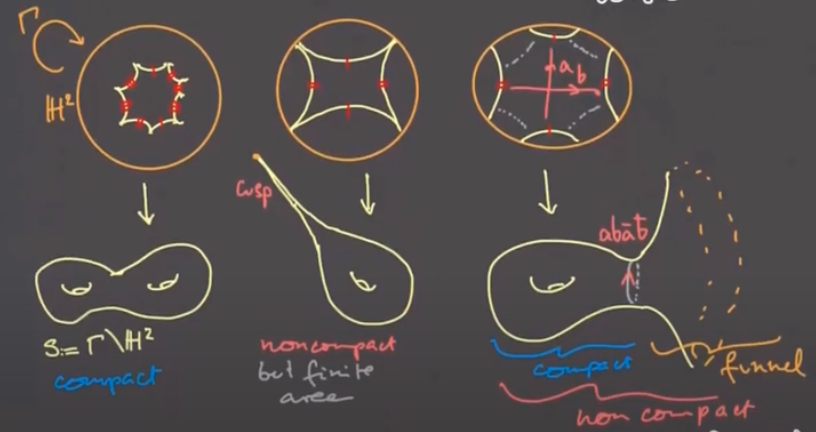
\includegraphics[width=0.7\textwidth]{proper actions.png}
    \caption{Proper actions on hyperbolic disk}
    \label{fig:proper_actions}
\end{figure}
\subsubsection{Convex cocompactness and Anosovness}
Recall that a representation is almost faithful if the kernel is finite.
The following proposition tells us that for $\SO_0(n,1)$ convex cocompactness and $P_1$-Anosov are equivalent and shows how we can obtain the limit map from the convex cocompactness condition.
\begin{theorem}\label{thm:convex_cocompact_anosov}
    Let $\rho: \Gamma \to \SO_0(n,1)$ be a representation of a finitely generated group $\Gamma$.
    Then $\rho$ is convex cocompact if and only if it is $P_1$-Anosov.
    In that case:
    \begin{enumerate}[label=(\roman*)]
        \item $\Gamma$ is Gromov hyperbolic.
        \item $\rho$ is discrete and almost faithful.
        \item There exists a continuous, injective, $\rho$-equivariant map $\xi: \partial \Gamma \to \partial \mathbb H^n$ that is dynamics-preserving, i.e.\ we have 
        $$\lim_{n \to \infty} \rho(\gamma_n) x = \xi(z)$$
        for sequences $\gamma_n \in \Gamma$ such that $\gamma_n \to z \in \partial \Gamma$ and points $x \in \mathbb H^n$.
        Moreover, for elements $\gamma \in \Gamma$ of infinite order, $\rho(\gamma)$ fixes $\xi(\gamma^+)$ and $\xi(\gamma^-)$.
    \end{enumerate}
\end{theorem}
\begin{proof}
    We fix throughout the proof an element $x_0 \in \mathbb H^n$ and consider the orbit map corresponding to it.
    The hyperbolicity of $\Gamma$ follows from the lemma of Milnor-Svarc.
    To prove that $\rho$ is discrete, we proceed by contradiction. If this were not the case, then there would exist a sequence $\gamma_n \in \Gamma$ with no repeated elements such that $\rho(\gamma_n) \to e$.
    In particular, $\rho(\gamma_n) x_0$ is bounded.
    Since the orbit map is a quasi-isometric embedding, this implies that $|\gamma_n|$ is bounded, which is a contradiction, since this would imply that $\{\gamma_n\}$ is finite.
    Similarly, to show that $\rho$ is almost faithful, we can show that the kernel is bounded, and hence finite.

    For the second point, the lemma of Milnor-Svarc implies that the orbit map is a quasi-isometry, and the theory of Gromov hyperbolic spaces, we know that it must extend to a homeomorphism $\xi: \partial \Gamma \to \partial \mathbb H^n$ between the Gromov boundaries.
    Let $\gamma_n \in \Gamma$ converge to $z \in \partial \Gamma$. 
    By Milnor-Svarc, we have that $\rho(\gamma_n)^{n} x_0 \to \xi(z)$ as $n \to \infty$.
    But for any $x \in \mathbb H^n$, we have that $d(\rho(\gamma_n) x_0, \rho(\gamma_n) x) = d(x_0, x)$ is bounded, and $\rho(\gamma_n) x_0 \to \xi(z)$ as $n \to infty$, so $\rho(\gamma_n) x \to \xi(z)$ by  \cref{lem:bounded_distance_convergence}.
    In particular, for an infinite order element $\gamma \in \Gamma$, we have that $\gamma^{\pm n} \to \gamma^\pm$ as $n \to \infty$, so $\rho(\gamma^n) x_0 \to \xi(\gamma^\pm)$.
    Since $\xi(\gamma^\pm)$ is the limit of a sequence fixed by $\rho(\gamma)$, it will be fixed as well.
\end{proof}
\subsubsection{Limit set}
\begin{definition}
    Let $H$ be a discrete subgroup of $\SO_0(n,1)$.
    Then the limit set $\Lambda$ of $H$ is the set of accumulation points of an orbit of $H$ that are contained in $\partial \mathbb H^n$:
    \[
    \Lambda = \overline{H x_0} - H x_0 \subseteq \partial \mathbb H^n,
    \]
    where $x_0 \in \mathbb H^n$ is fixed.
\end{definition}
\begin{remark}
    In the above definition, there have been made a few subtle assertions:
    \begin{enumerate}[label=(\roman*)]
        \item The limit set $\Lambda(\rho)$ is independent of the choice of $x_0$.
        This can be seen by using \cref{lem:bounded_distance_convergence}.
        \item The set of accumulation points in $\partial \mathbb H^n$ of an orbit is equal to $\overline{H x_0} - H x_0$.
        Clearly the set of accumulation points is contained in $\overline{H x_0}$.
        To see that it is disjoint from $H x_0$, we can use the fact that it is contained in $\partial \mathbb H^n$.
        On the other hand, every element in $\overline{H x_0} - H x_0$ is the limit of a sequence of discrete elements in $H$, so it is an accumulation point.
        \item \label{rem:limit_set_properly_discontinuous}If one assumes that $H$ is a discrete subgroup that acts properly discontinuously on $\mathbb H^n$, then the accumulation points of any orbit lie on the boundary of $\mathbb H^n$.
        To see this, assume for the sake of contradiction that there exists an accumulation point $z \in \mathbb H^n$ of an orbit $H x_0$.
        Then there exists a sequence of pairwise different elements $h_n \in H$ such that $h_n x_0 \to z$.
        In particular $h_n x_0$ is bounded, so there exists some ball $B_R(x_0)$ that contains all $h_n x_0$ and $x_0$.
        This however implies that $h_n x_0 \in h_n B_{R}(x_0) \cap B_R(x_0)$ for all $n$, which contradicts thes proper discontinuity of the action.
    \end{enumerate}
\end{remark}
Now we are ready to make the link between the geometric definition of convex cocompactness and the notion of convex cocompact representation (i.e.\ a representation whose orbit map is a quasi-isometric embedding).
\begin{proposition}\label{prop:convex_cocompact_limit_set}
    Let $\rho: \Gamma \to \SO_0(n,1)$ be a discrete and faithful representation.
    Then $\rho$ is convex cocompact if and only if $\rho(\Gamma)$ preserves a convex subset of $\mathbb H^n$, on which it acts cocompactly.
    In that case, the convex hull of the limit set $\Lambda(\rho)$ of $\rho(\Gamma)$ is such a subset.
\end{proposition}
\subsubsection{Stability and closedness}
Two of the basic features of the space of convex cocompact representations that we look for when generalizing are their stability and closedness.
To fix our notation, for a group $\Gamma$ we denote with $\mathrm{CC}(\Gamma, \SO_0(n,1)) \subseteq \hom(\Gamma, \SO_0(n,1))$ the set of convex cocompact representations of $\Gamma$ in $\SO_0(n,1)$, with $\mathrm{X}(\Gamma, \SO_0(n,1)) = \hom(\Gamma, \SO_0(n,1))/\SO_0(n,1)$ the character variety of $\Gamma$ in $\SO_0(n,1)$, and with $\hat{\mathrm{CC}}(\Gamma, \SO_0(n,1)) \subseteq \mathrm{X}(\Gamma, \SO_0(n,1))$ the set of conjugacy classes of convex cocompact representations.
We will also denote with $\mathrm{DF}(\Gamma, \SO_0(n,1)) \subseteq \hom(\Gamma, \SO_0(n,1))$ the set of discrete and faithful representations and with $\hat{\mathrm{DF}}(\Gamma, \SO_0(n,1)) \subseteq \mathrm{X}(\Gamma, \SO_0(n,1))$ the set of conjugacy classes of discrete and faithful representations.
Then we have:
\begin{theorem}\cref{thm:stability_closedness}
    Let $\Gamma$ be a finitely generated group.
    \begin{enumerate}[label=(\roman*)]
        \item The convex cocompact representations of $\Gamma$ are open in the space of representations and in the character variety, i.e.\ 
        \[
        \mathrm{CC}(\Gamma, \SO_0(n,1)) \subseteq \hom(\Gamma, \SO_0(n,1)) \text{ and } \hat{\mathrm{CC}}(\Gamma, \SO_0(n,1)) \subseteq \mathrm{X}(\Gamma, \SO_0(n,1))
        \]
        are open.
        \item If we assume that $\Gamma$ is torsion-free and not virtually cyclic, then the convex cocompact representations are closed in the space of representations and in the character variety, i.e.\
        \[
        \mathrm{CC}(\Gamma, \SO_0(n,1)) \subseteq \hom(\Gamma, \SO_0(n,1)) \text{ and } \hat{\mathrm{CC}}(\Gamma, \SO_0(n,1)) \subseteq \mathrm{X}(\Gamma, \SO_0(n,1))
        \]
        are closed.
    \end{enumerate}
\end{theorem}
\section{Various facts}
\begin{proposition}
    Let $\Gamma$ be a discrete group and $\rho: \Gamma \to G$ be a $P_\Theta$-Anosov in a semisimple Lie group $G$.
    Then the image $\rho(\Gamma)$ is discrete.
\end{proposition}
\begin{proof}
    Suppose $\rho(\Gamma)$ were not discrete.
    Since $G$ is Hausdorff, this is equivalent to the existence of a sequence ${\rho(\gamma_n)}_n$ of distinct elements of $\rho(\Gamma)$ such that $\rho(\gamma_n) \to e$.
    In particular, $\gamma_n$ is a sequence of distinct elements of $\Gamma$.
    But by the continuity of the Cartan projection, we have that $\alpha(\mu(\rho(\gamma_n))) \to \alpha(\mu(e)) = 0$, for $\alpha \in \Theta$.
    Hence the sequence $\mu(\rho(\gamma_n))$ is bounded, which given the $P_\Theta$-Anosov property of $\rho$, means that the word-lengths of ${\gamma_n}_n$ are bounded.
    However, this implies that the sequence ${\gamma_n}_n$ is finite, which is a contradiction.
\end{proof}

\chapter{Lorentzian spaces}
Here we recall some basic facts on Lorentzian spaces.
We will introduce Lorentzian manifolds of constant sectional curvature and we will see that, as in the Riemannian case, two Lorentzian manifolds of constant sectional curvature $K$ are locally isometric.
Generally, we will focus on those with maximal isometry group, as they provide models of manifolds of constant sectional curvature: if $M$ is a Lorentzian manifold with constant sectional curvature $K$ and maximal isometry group, then any Lorentzian manifold with constant sectional curvature $K$ carries a natural $(\mathrm{Isom}(M), M)$-atlas made of local isometries. Simply connected space forms have maximal isometry group, but in general there are manifolds with maximal isometry group which are not simply connected.
In particular, we will focus on the case $K=-1$ and in that case it will be convenient to use  models which are not simply connected.

\section{Basic definitions}
\begin{definition}
    \begin{enumerate}[label=(\roman*)]
        \item A \emph{Lorentzian metric} on a manifold of dimension $n+1$  is a non-degenerate symmetric 2-tensor $g$ of signature $(n,1)$. 
        \item A \emph{Lorentzian manifold} is a connected manifold $M$ equipped with a Lorentzian metric $g$.
        \item In a Lorentzian manifold $M$ we say that a non-zero vector $v\in TM$ is \emph{spacelike, lightlike, timelike} if $g(v,v)$ is respectively positive, zero or negative. More generally, we say that a linear subspace $V\subset T_x M$ is \emph{spacelike, lightlike, timelike} if the restriction of $g_x$ to $V$ is positive definite, degenerate or indefinite.
        \item A differentiable curve is \emph{spacelike, lightlike, timelike} if its tangent vector is spacelike (resp. lightlike, timelike) at every point. It is \emph{causal} if the tangent vector is either timelike or lightlike.
        \item The set of lightlike vectors of $T_x M$ is also known as the \emph{light cone} at $x$.
    \end{enumerate}
\end{definition}

Assuming $\dim M \geq 3$, the light cone disconnects $T_x M$ into three regions: two convex open cones formed by timelike vectors, one opposite to the other, and the region of spacelike vectors.
\begin{definition}
    Let $M$ be a Lorentzian manifold.
    \begin{enumerate}[label=(\roman*)]
        \item A continuous choice (in the sense of a continuous timelike vector field) of one of the two cones of time-like vectors for each point $x\in M$ is called a \emph{time orientation} of $M$.
        \item If a time-orientation of $M$ exists, then $M$ is said to be \emph{time-orientable}.
        Timelike vectors in the same component as the time-orientation are said \emph{future-directed}, while the rest are said \emph{past-directed}.
        \item Given a point $x$ in a time-oriented Lorentzian manifold $M$, the \emph{future} of $x$ is the set $\fut{(x)}$ of points which are connected to $x$ by a future-directed causal curve. The \emph{past} of $x$, denoted $\past{(x)}$, is defined similarly, for past-directed causal curves.
    \end{enumerate}
\end{definition}

An \emph{orthonormal basis} of $T_xM$ is a basis $v_1,\ldots v_{n+1}$ such that $|g(v_i, v_j)|=\delta_{ij}$, with $v_1,\ldots v_n$ spacelike, and  $v_{n+1}$ timelike.
As in the Riemannian setting, on a Lorentzian manifold $M$ there is a unique linear connection $\nabla$ which is symmetric and compatible with the Lorentzian metric $g$.
We refer to it as the \emph{Levi-Civita connection} of $M$. The Levi-Civita connection determines the Riemann curvature tensor  defined by
$$R(u,v)w=\nabla_u \nabla_v w-\nabla_v \nabla_u w-\nabla_{[u,v]}w~.$$
We then say that a Lorentzian manifold $M$ has constant sectional curvature $K$ if
\begin{equation}\label{eq:constcurv}
     g(R(u,v)v,u)=K \left(g(u,u)g(v,v)-g(u,v)^2\right)
\end{equation}
for every pair of vectors $u,v\in T_xM$ and every $x\in M$.
This definition is strictly analogous to the definition given in the Riemannian realm. However in this setting the sectional curvature can be defined only for planes in 
$T_x M$ where $g$ is non-degenerate.
\begin{example}
The Minkowski space $\R^{n,1}$ the Levi-Civita connection given by the Euclidean connection:
\[
\nabla_X Y = (X Y^i)\partial_i,
\]
so the Riemann curvature tensor is zero, and the same is true for the sectional curvature.
\end{example}

Finally, we say that $M$ is \emph{geodesically complete} if every geodesic is defined for all times, or in other words, the exponential map is defined everywhere.

\section{Maximal isometry groups and geodesic completeness}
Constant curvature of manifolds allows us to extend isometries of tangent spaces to isometries of the whole manifold.
As a result, two Lorentzian manifolds $M$ and $N$ of constant curvature $K$ are locally isometric, a fact which is well-known in the Riemannian setting. 
More precisely, the following holds:
\begin{lemma} \label{lem:extension}
Let $M$ and $N$ be Lorentzian manifolds of constant curvature $K$. 
\begin{enumerate}
    \item Then every linear isometry $L:T_xM\to T_yN$ extends to an isometry $f:U\to V$, where $U$ and $V$ are neighbourhoods of $x$ and $y$ respectively, and two extensions $f:U\to V$ and $f:U'\to V'$ of $L$ coincide on $U\cap U'$.
    \item If $M$ is simply connected and $N$ is geodesically complete, then any isometry $L: T_x M \to T_y N$ extends to a unique local isometry $f:M\to N$.
    \item If $M$ and $N$ are both simply connected and geodesically complete, then any isometry $L: T_xM\to T_yN$ extends to a unique global isometry $f:M\to N$.
\end{enumerate}
\end{lemma}
\begin{proof}
    For the last statement, recall that a local isometry from a simply connected manifold to a uniquely geodesic manifold is a global isometry.
\end{proof}
Exactly as in the Riemannian case the proof is a simple consequence of the classical Cartan--Ambrose--Hicks Theorem.
Note that this implies in particular that there is a unique simply connected geodesically complete Lorentzian manifold of constant curvature $K$ up to isometries.
For instance for $K=0$ a model is the Minkowski space $\R^{n,1}$.

Another consequence of Lemma \ref{lem:extension} is that, fixing a point $x_0\in M$, the set of isometries of $M$, which we will denote by $\mathrm{Isom}(M)$, can be realized as a subset of $\mathrm{ISO}(T_{x_0}M, TM)$, namely the fiber bundle over $M$ whose fiber over $x\in M$ is the space of linear isometries of $T_{x_0}M$ into $T_x M$.

It can be proved that $\mathrm{Isom}(M)$ has the structure of a Lie group with respect to composition so that the inclusion
$\mathrm{Isom}(M)\hookrightarrow\mathrm{ISO}(T_{x_0}M, TM)$ is a differentiable proper embedding.
It follows that  the maximal dimension of $\mathrm{Isom}(M)$ is
 $\dim \OO(n,1)+n+1=(n+1)(n+2)/2$. 
 
\begin{definition}
A Lorentzian manifold $M$ has \emph{maximal isometry group} if the action of $\mathrm{Isom}(M)$ is transitive and, 
for every point $x\in M$, every linear isometry $L:T_xM\to T_xM$ extends to an isometry of $M$.
\end{definition}
Equivalently $M$ has maximal isometry group if the above inclusion of $\mathrm{Isom}(M)$ into the bundle $\mathrm{ISO}(T_{x_0}M, TM)$ is a bijection.
Hence, if $M$ has maximal  isometry group, then the dimension of the isometry group is maximal.

From \cref{lem:extension}, every simply connected Lorentzian manifold $M$ has maximal isometry group if it has constant sectional curvature and is geodesically complete. The converse holds even without the simply connectedness assumption:
\begin{lemma} \label{lemma:max isom group implies constant curvature}
\begin{enumerate}[label=(\roman*)]
    Let $M$ be a Lorentzian manifold.
    \item If $M$ has a maximal isometry group then $M$ has  constant sectional curvature and is geodesically complete.
    \item If $M$ is simply connected, then $M$ has maximal isometry group if and only if $M$ has constant sectional curvature and is geodesically complete.
\end{enumerate}
\end{lemma}

\chapter{Pseudoriemannian hyperbolic spaces}
\begin{definition}
    Let $V$ be a real vector space of dimension $n = p+q+1$, equipped with an inner product $\langle \cdot, \cdot \rangle$ of signature $(p,q+1)$.
    We define the pseudoriemannian hyperbolic space
    \[
    \mathbb H^{p,q} = \left\{ x \in \mathbb P(V) : \langle x,x \rangle < 0\right\},
    \]
    whose double cover is given by 
    \[
    \hat{\mathbb H}^{p,q} = \left\{ x \in V : \langle x,x \rangle = -1 \right\}
    \]
\end{definition}
\section{Second fundamental form}
A reference for the material of this section is Chapter 4 of \cite{o1983semi}.
When we say submanifold, we mean embedded (the inclusion is an emersive topological embedding).
\begin{definition}
    Let $M$ be a pseudoriemannian submanifold of a pseudoriemannian manifold $\tilde M$.
    Then the orthogonal decomposition of the tangent bundle $TM$ with respect to the ambient metric defines two vector bundle homomorphisms: 
    \[
    \nabla : \Gamma(M) \times \Gamma(M) \to \Gamma(TM),\quad \II: \Gamma(TM) \to \Gamma(NM), 
    \]
    that satisfy
    \[
    \tilde \nabla_X Y = \nabla_X Y + \II(X,Y), \text{ for } X,Y \in \Gamma(TM),
    \]
    where $\tilde nabla$ is the Levi-Civita connection of $\tilde M$ and $\tilde nabla_X Y$ is evaluated for any smooth extensions of $X,Y$ to $\tilde M$.
    The first is called the induced connection on $M$ and the second is called the second fundamental form of $M$ in $\tilde M$.
\end{definition}
The notation $\nabla$ is understood in the light of the following proposition.
\begin{proposition}
    Let $M$ be a pseudoriemannian submanifold of a pseudoriemannian manifold $\tilde M$.
    Then the induced connection $\nabla$ is the Levi-Civita connection of $M$ with respect to the induced metric.
\end{proposition}
The second fundamental form has a few basic properties:
\begin{proposition}
    Let $M$ be a pseudoriemannian submanifold of a pseudoriemannian manifold $\tilde M$.
    Then the second fundamental form $\II$ satisfies the following properties:
    \begin{enumerate}[label=(\roman*)]
        \item Symmetry: $\II(X,Y) = \II(Y,X)$ for all $X,Y \in \Gamma(TM)$.
        \item Biliniearity: $\II$ is bilinear in $C^\infty(M)$.
        \item The value of $II(X,Y)$ at $p \in M$ for $X, Y \in \Gamma(TM)$ depends only on the values of $X_p, Y_p$ at $p$.
    \end{enumerate}
\end{proposition}
Hence, to compute the Levi-Civita connection of a pseudoriemannian submanifold, it suffices to project the Levi-Civita connection of the ambient space onto the tangent space of the submanifold, or equivalently, compute the second fundamental form of $M$.
Similarly, there exists an analog of the Gauss formula for vector fields over curves:
\begin{proposition}
    Let $M$ be a pseudoriemannian submanifold of a pseudoriemannian manifold $\tilde M$, $\gamma: I \to M$ a smooth curve in $M$ and $X \in \Gamma(\gamma)$ a smooth vector field along $\gamma$ (with values in $TM$).
    Then 
    \[
    \tilde D_t X = D_t X + \II(\gamma', X),
    \]
    where $\tilde D_t X$ is the covariant derivative along $\gamma$ in $M$ of an extension of $X$ on $M$, $D_t$ is the covariant derivative along $\gamma$ in the submanifold.
\end{proposition}
\begin{remark}
    The Gauss formula for vector fields and curves give us two ways of interpreting the second fundamental form.
    If $(M, g)$ is a pseudoriemannian submanifold of a pseudoriemannian manifold $(\tilde M, \tilde g)$, then
    \begin{enumerate}
        \item The second fundamental form measures the difference between differentiation in the ambient space $\tilde M$ and differentiation in the submanifold $M$ for given vector fields in $M$.
        \item $\II(v,v)$ is the $\tilde g$-acceleration $\tilde D_t \tilde \gamma$ of the $g$-geodesic $\gamma$ in $M$, with initial veolicity $v \in T_p M$.
    \end{enumerate}
\end{remark}
The second fundamental form can give us the curvature of a submanifold:
\begin{proposition}\label{prop:curvature_submanifold}
    Let $M$ be a pseudoriemannian subbmanifold of a pseudoriemannian manifold $M$.
    Then for every $v, w \in T_p M$ that generate a nondegenerate plane, the sectional curvature of $M$ is given by
    \[
    K(v,w) = \tilde K(v,w) + \frac{\langle \II(v,v) ,\II(w,w) \rangle - \langle \II(v,w), \II(v,w) \rangle^2}{ \langle v,v \rangle \langle w,w \rangle - \langle v,w \rangle^2}.
    \]
\end{proposition}
\subsection{Pseudoriemannian hypersurfaces}
Let $M$ be a pseudoriemannian hypersurface of a pseudoriemannian manifold $\tilde M$.
Around every point, we can define a unit normal vector field $N$ that is orthogonal to the tangent space of $M$.
\begin{figure}[ht]
    \centering
    \begin{tabular}{cc}
        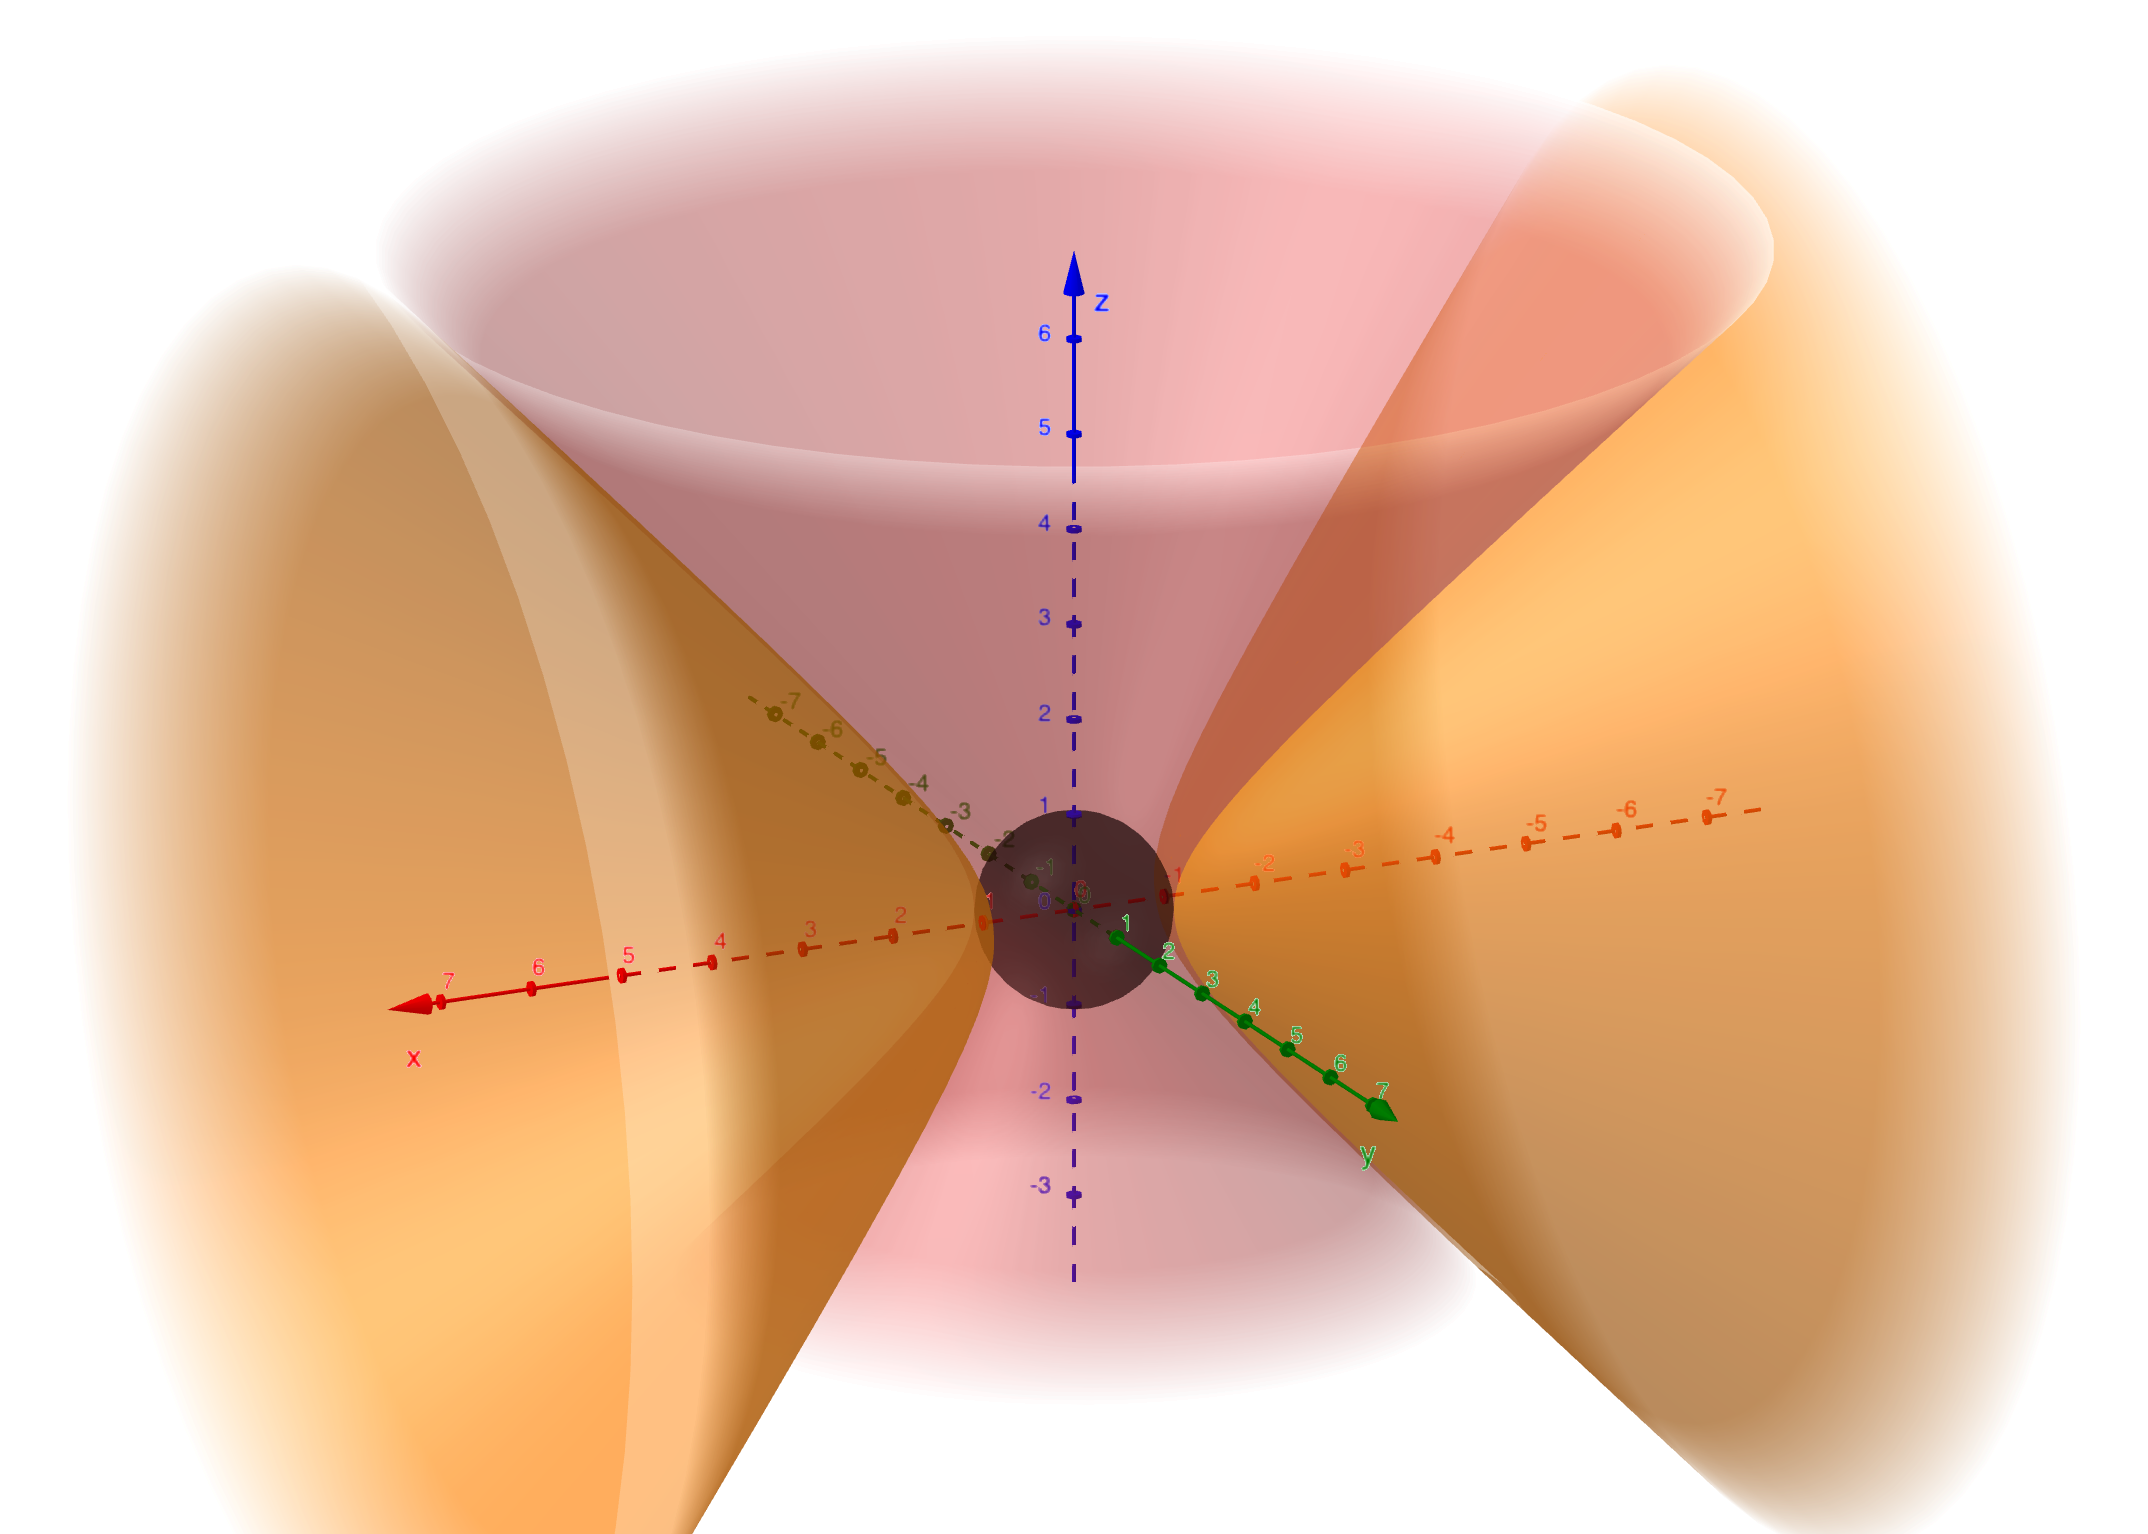
\includegraphics[width=0.45\textwidth]{Pseudospheres/pseudospheres.png} &
        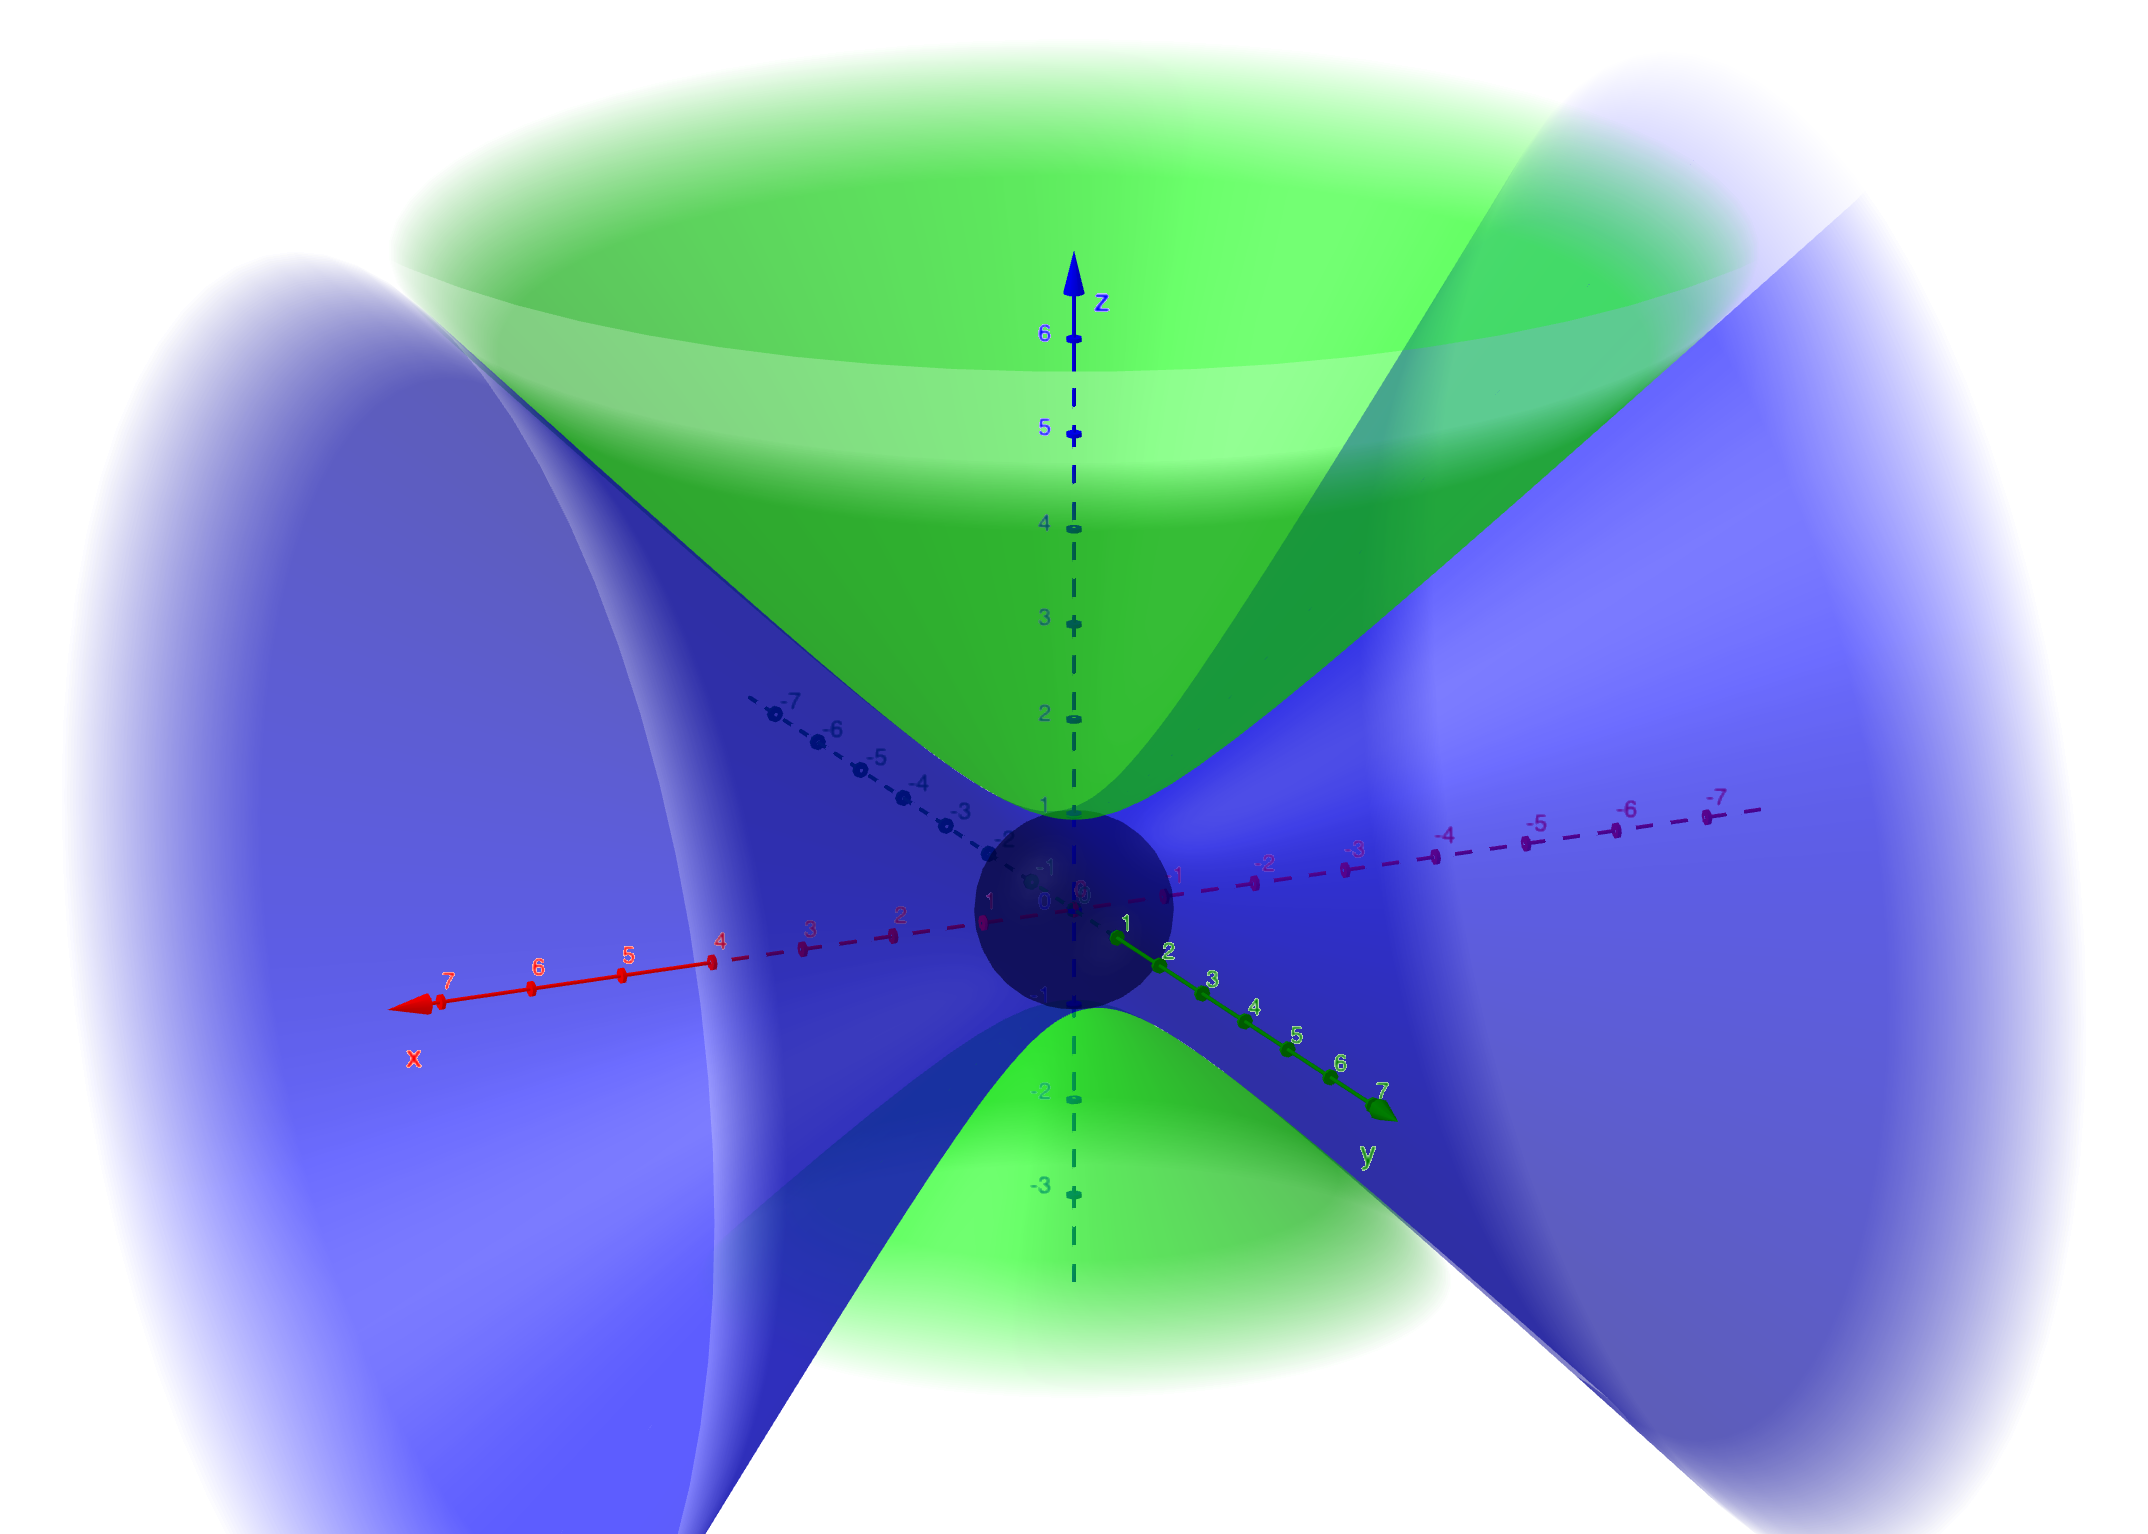
\includegraphics[width=0.45\textwidth]{Pseudospheres/pseudohyperbolics.png} \\
        \small (a) Pseudospheres in different signatures  &
        \small (b) Pseudohyperbolics in different signatures \\
        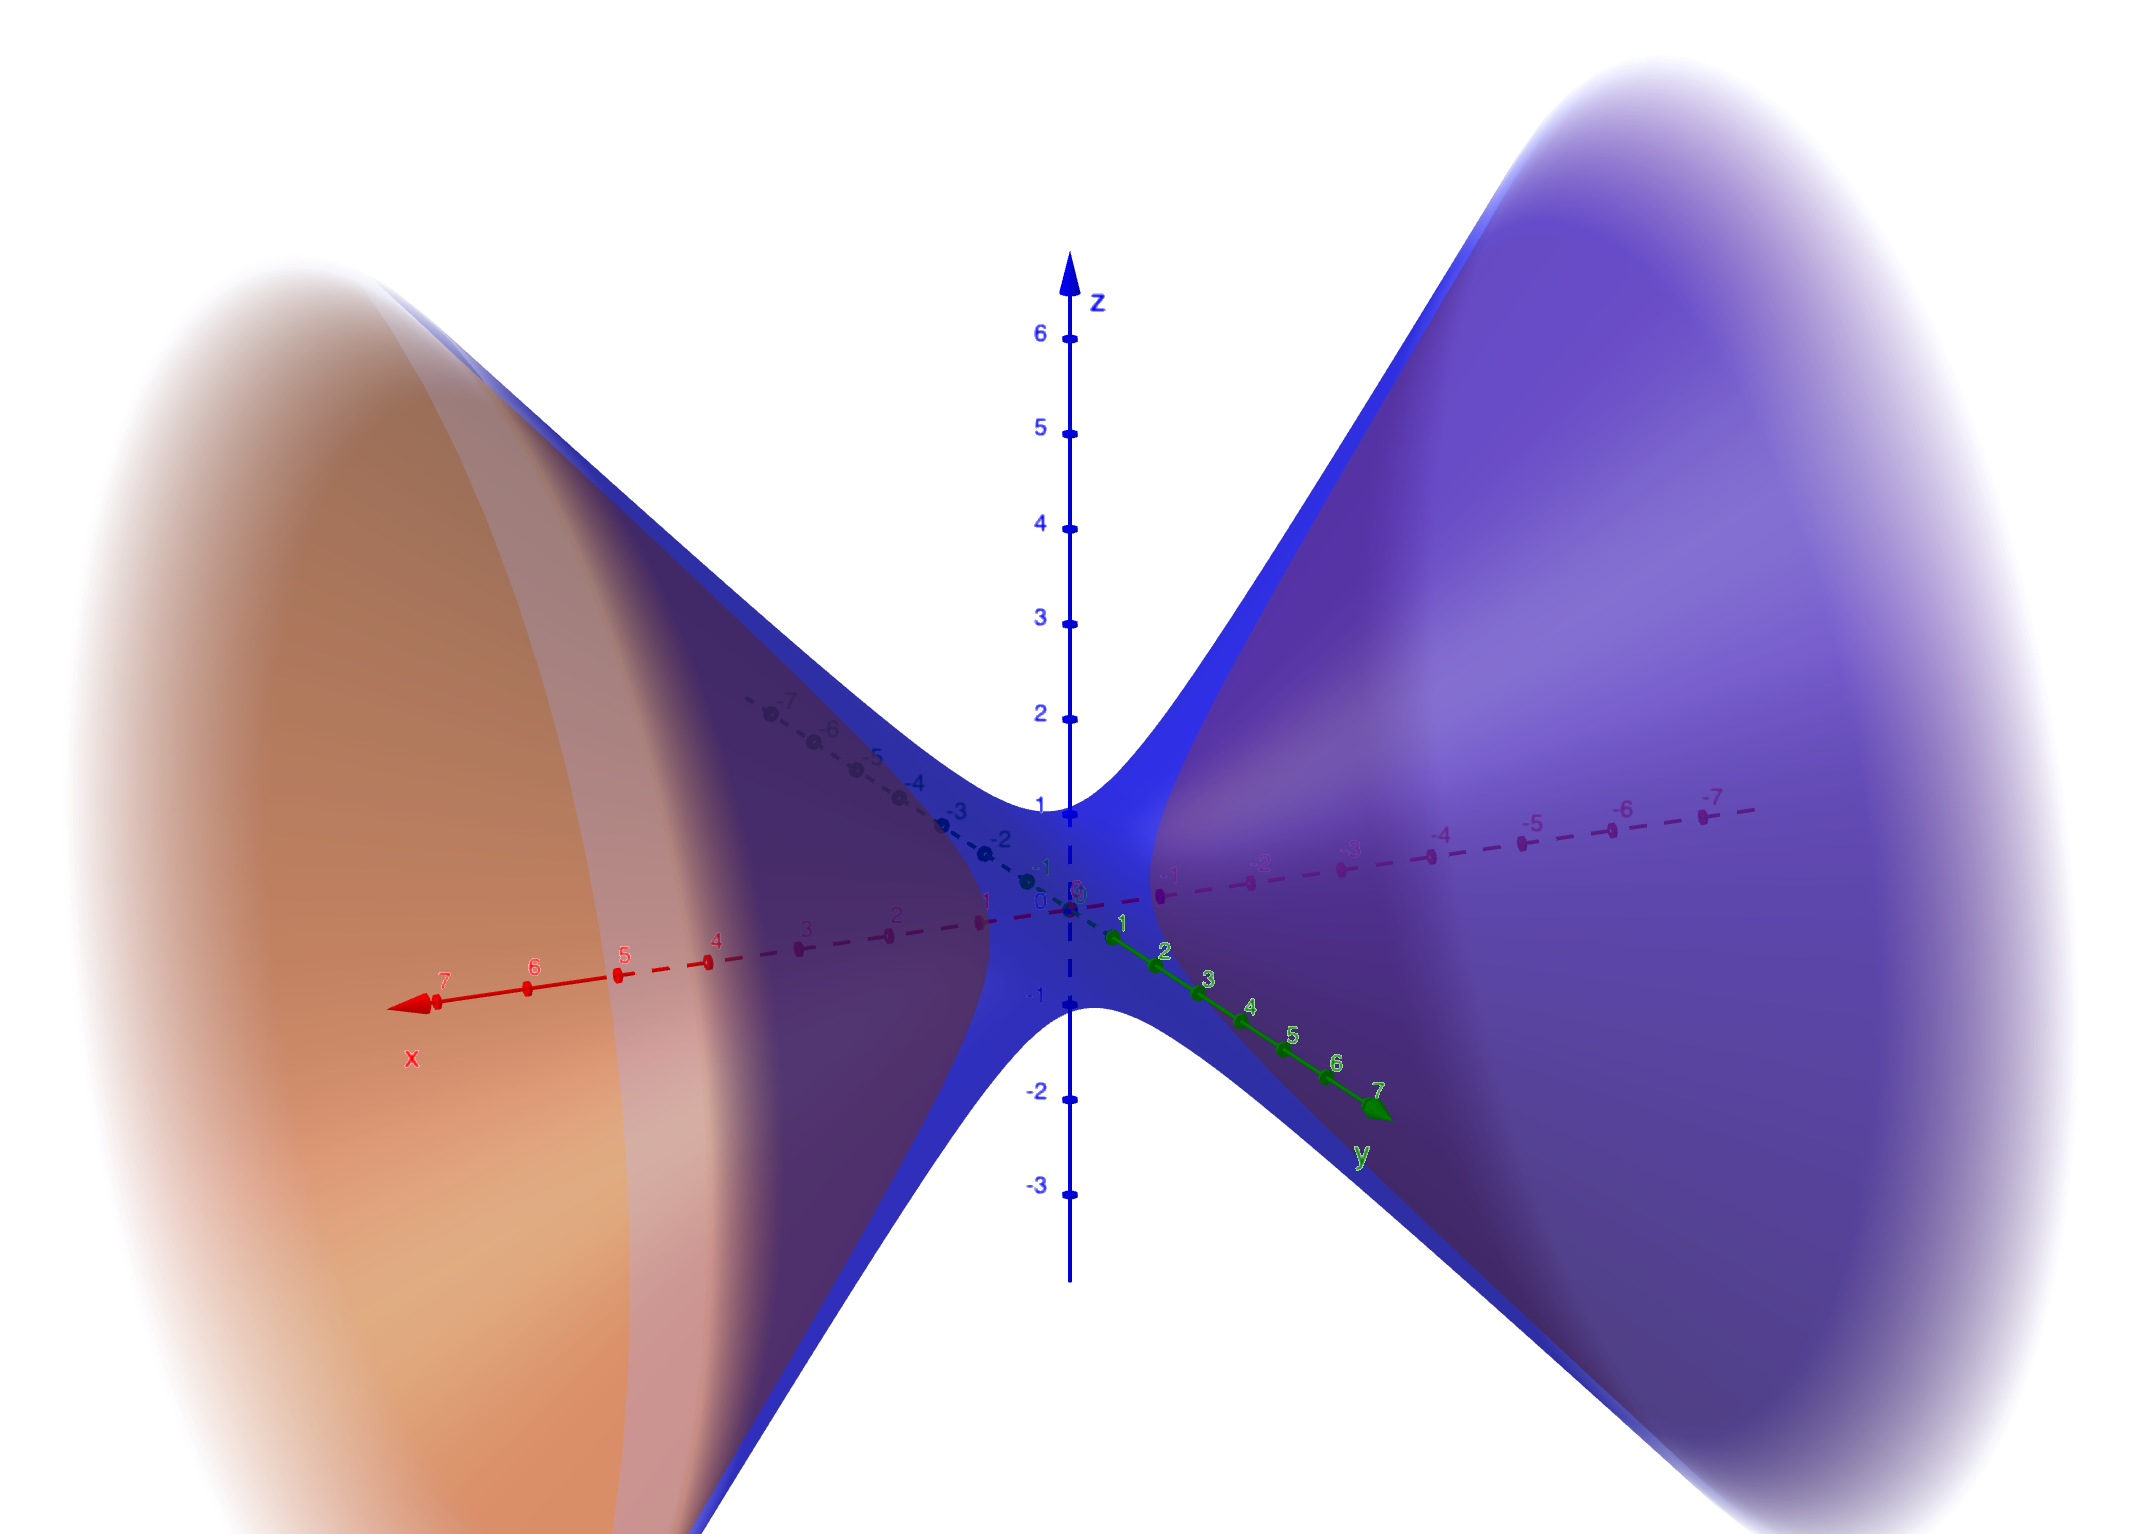
\includegraphics[width=0.45\textwidth]{Pseudospheres/H_1_1_S_0_2.png} &
        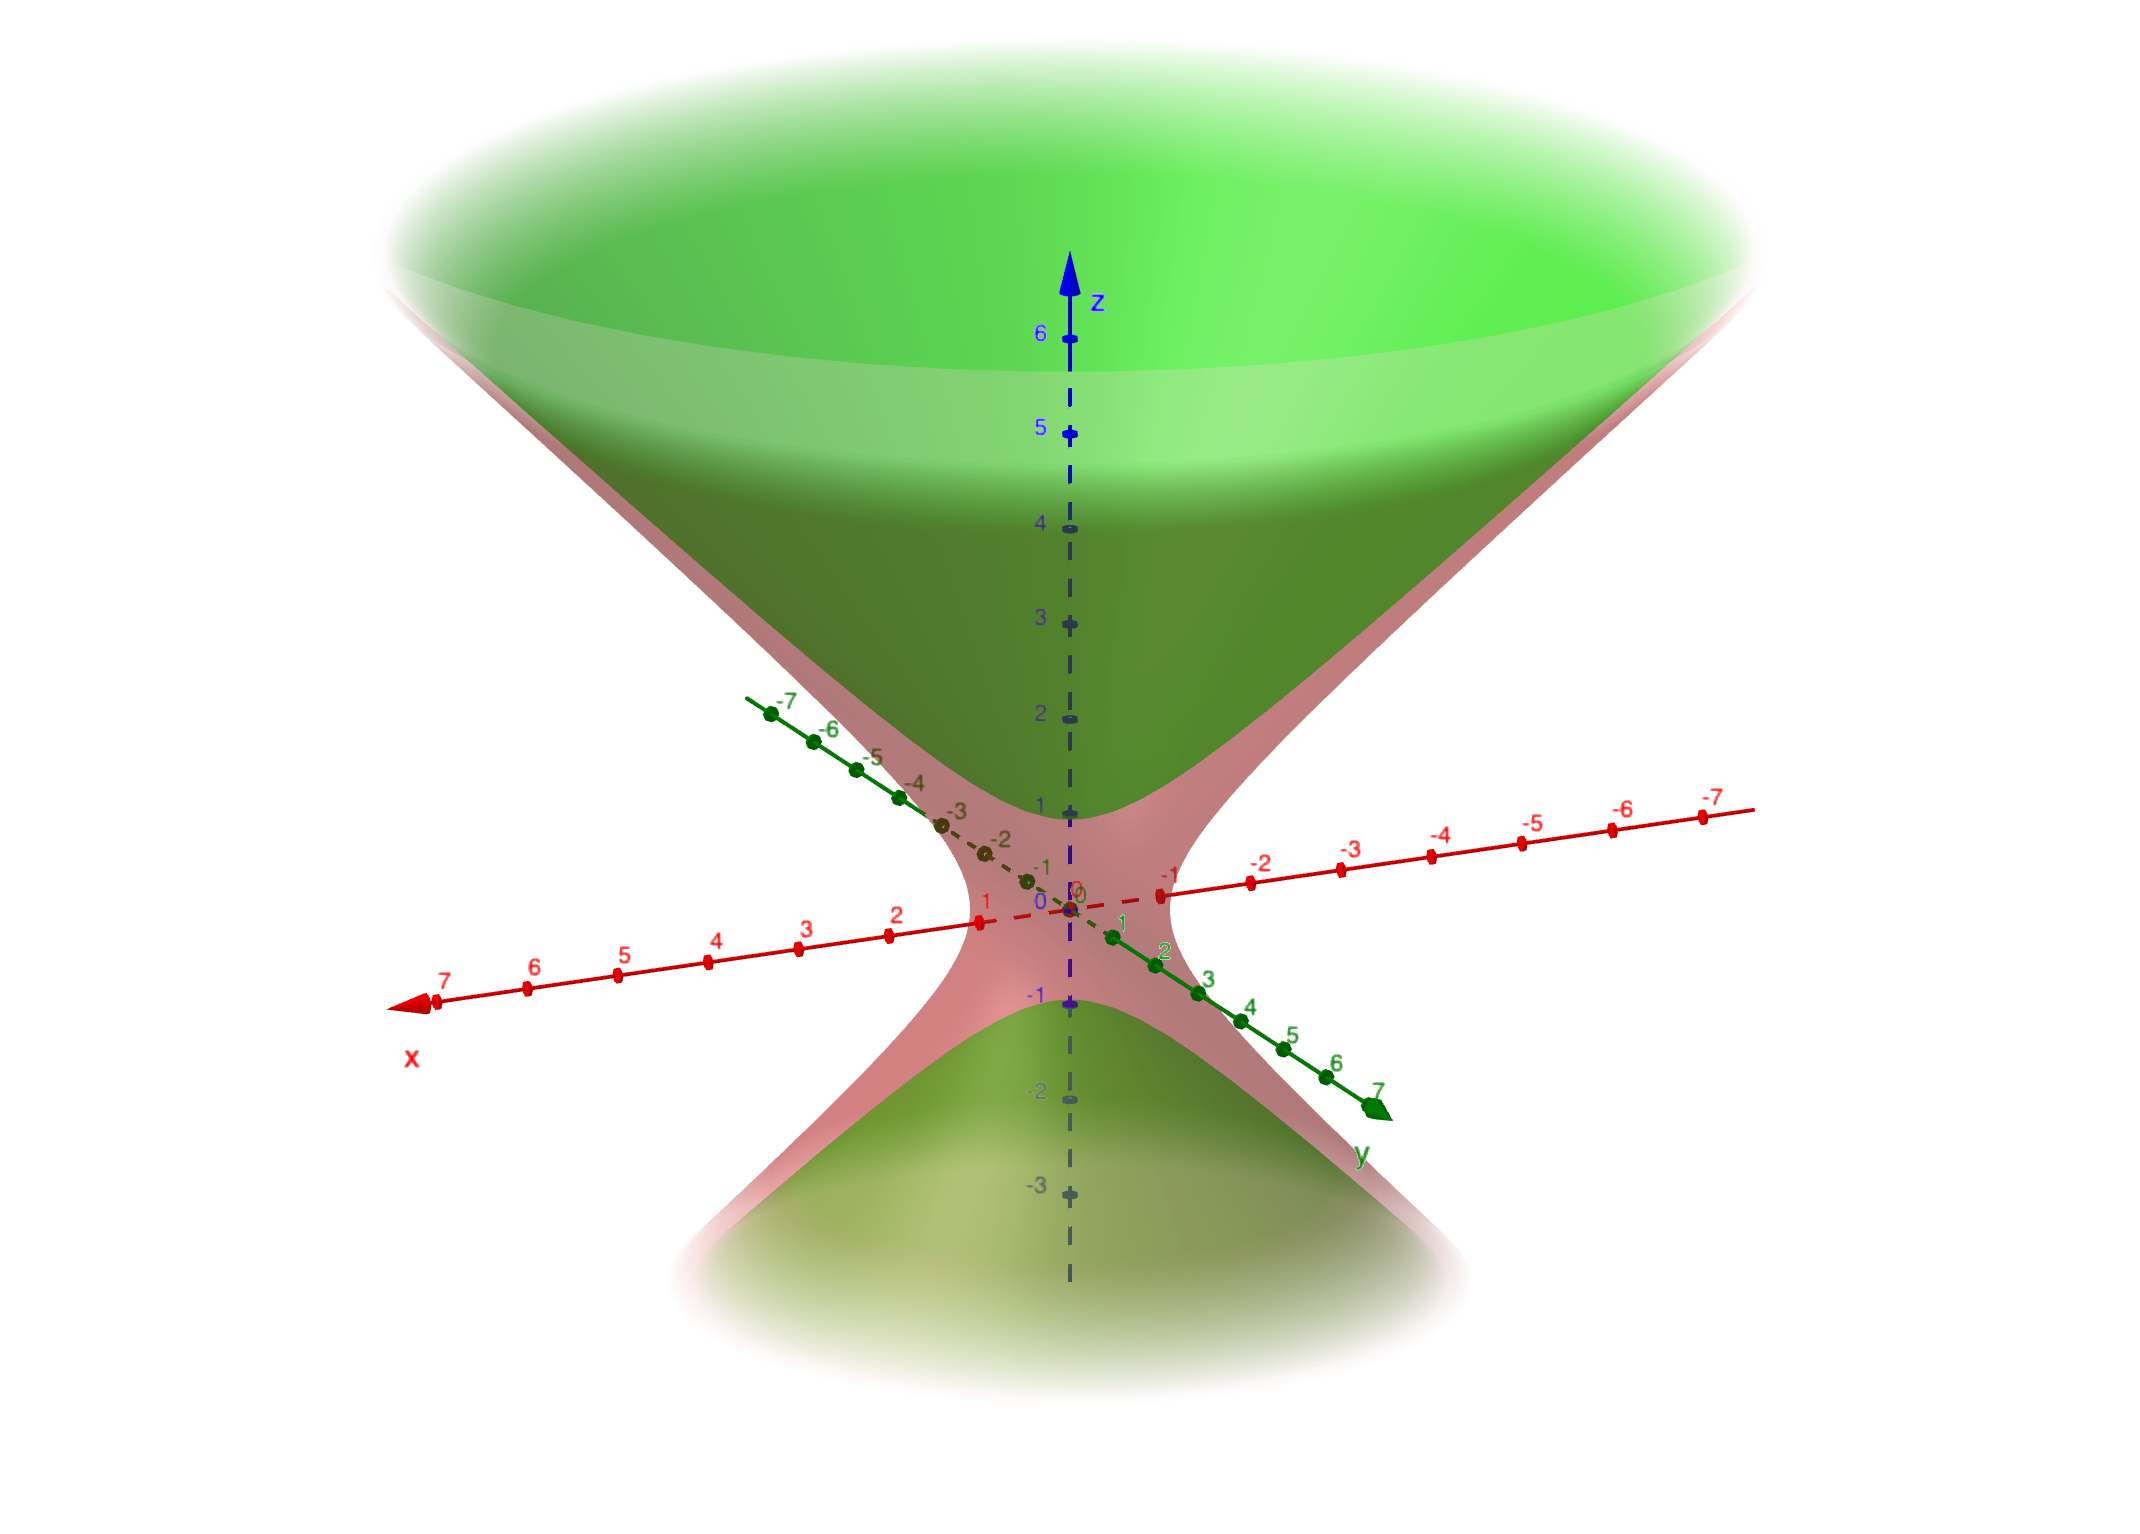
\includegraphics[width=0.45\textwidth]{Pseudospheres/H_2_0_S_1_1.png} \\
        \small (c) $\mathbb H^{1,1}$ and $\mathbb S^{0,2}$ &
        \small (d) $\mathbb H^{2,0}$ and $\mathbb S^{1,1}$
    \end{tabular}
    \caption{Visualizations of pseudospheres and pseudohyperbolics in different signatures,\\ $\mathbb S^{2,0}$: black, $\mathbb S^{1,1}$: red, $\mathbb S^{0,2}$: orange, $\mathbb H^{2,0}$: green, $\mathbb H^{1,1}$: blue, $\mathbb H^{0,2}$: black, \href{https://www.geogebra.org/m/rwsndb8h}{Geogebra applet}.}
    \label{fig:pseudospheres_grid}
\end{figure}
\begin{definition}
    Let $M$ be a pseudoriemannian hypersurface of a pseudoriemannian manifold $\tilde M$, and let $N$ be a unit normal vector field.
    We define the shape operator $s: \Gamma(TM) \to \Gamma(TM)$ with respect to $N$ by
    \[
    \langle s X, Y \rangle = \langle \II(X,Y), N \rangle, \text{ for } X,Y \in \Gamma(TM).
    \]
    It can often by computed using the formula
    \[
    s X = \tilde \nabla_X N.
    \]
\end{definition}
The shape operator captures the second fundamental form of the hypersurface in the following sense:
\[
\II(X,Y) = \langle N, N \rangle \langle s X, Y \rangle N.
\]
Analogously to \cref{prop:curvature_submanifold}, the shape operator can give us the curvature of a hypersurface:
\begin{proposition}\label{prop:curvature_hypersurface}
    Let $M$ be a pseudoriemannian hypersurface of a pseudoriemannian manifold $M$.
    Then for every $v, w \in T_p M$ that generate a nondegenerate plane, the sectional curvature of $M$ is given by
    \[
    K(v,w) = \tilde K(v,w) + \langle N, N \rangle \frac{\langle Sv ,v \rangle \langle Sw, w \rangle- \langle Sv, w \rangle^2}{ \langle v,v \rangle \langle w,w \rangle - \langle v,w \rangle^2},
    \]
    where $N$ is the unit normal vector field, and $S$ is the shape operator with respect to $N$.
\end{proposition}
\subsubsection{Hyperquadrics}
We give the analogue of the sphere and the hyperbolic space for the pseudoriemannian case, i.e.\ the pseudoriemannian hypersurfaces of constant sectional curvature (see \cref{ex:hyperquadratics_curvatures}).
The notation $\mathbb S^{p,q}, \mathbb H^{p,q}$ hints to the signature of the induced metric.
\begin{definition}
    Let $0 \leq \nu \leq n$, with $n \geq 2$.
    We define the pseudosphere of radius $r > 0$ as
    \[
    \mathbb S^n_\nu(r) = \mathbb S^{n-\nu,\nu}(r) = \left\{ x \in \mathbb R^{n+1}_\nu = \mathbb R^{n+1-\nu,\nu} : \langle x,x \rangle = r^2 \right\},
    \]
    and the pseudohyperbolic space of radius $r > 0$ as
    \[
    \mathbb H^n_\nu(r) = \mathbb H^{n - \nu, \nu}(r) = \left\{ x \in \mathbb R^{n+1}_\nu = \mathbb R^{n-\nu, \nu + 1} : \langle x,x \rangle = -r^2 \right\}.
    \]
\end{definition}
\begin{example}\label{ex:hyperquadratics_curvatures}
    The shape operator for the pseudospheres $\mathbb S^{p,q}$ and on the pseudohyperbolic spaces is given $Sv = -\frac{1}{r} v$.
    In particular, the  pseudosphere $\mathbb S^{n - \nu, \nu}(r)$ is of constant sectional curvature $K = \frac{1}{r^2}$, and the pseudohyperbolic space $\mathbb H^{n - \nu, \nu}(r)$ is of constant sectional curvature $K = -\frac{1}{r^2}$.
\end{example}
As one can suspect, the pseudospheres and the pseudohyperbolics are related to each other:
\begin{proposition}
    The pseudospheres are anti-isometric to the pseudohyperbolic spaces.
    More precisely, the map
    \begin{align*}
        \sigma: \mathbb S^n_\nu(r) = \mathbb S^{n - \nu, \nu}(r) &\to \mathbb H^n_{n - \nu}(r) = \mathbb H^{\nu, n - \nu}(r)\\
        (x_1, \cdots x_\nu, x_{\nu+1}, \cdots x_{n+1}) &\mapsto (x_{\nu+1}, \cdots x_{n+1}, x_1, \cdots x_\nu)\\
    \end{align*}
    is an anti-isometry, i.e.\ a diffeomorphism that satisfies $\d_x \sigma (u), d_x \sigma (v) = -\langle u, v \rangle$ for all $u,v \in T_x \mathbb S^n_\nu(r)$.
\end{proposition}
We have also a simple diffeomorphic model for the pseudospheres and pseudohyperbolics:
\begin{proposition}
    Each $\mathbb S^n_\nu(r) = \mathbb S^{n - \nu, \nu}(r)$ is diffeomorphic to $\mathbb R^{\nu} \times \mathbb S^{n-\nu}$, and each $\mathbb H^n_\nu(r) = \mathbb H^{n - \nu, \nu}(r)$ is diffeomorphic to $\mathbb S^{\nu} \times \mathbb R^{n -\nu}$. 
\end{proposition}
The following proposition gives the geodesics of the pseudospheres and the pseudohyperbolics.
\begin{figure}[ht]
    \centering
    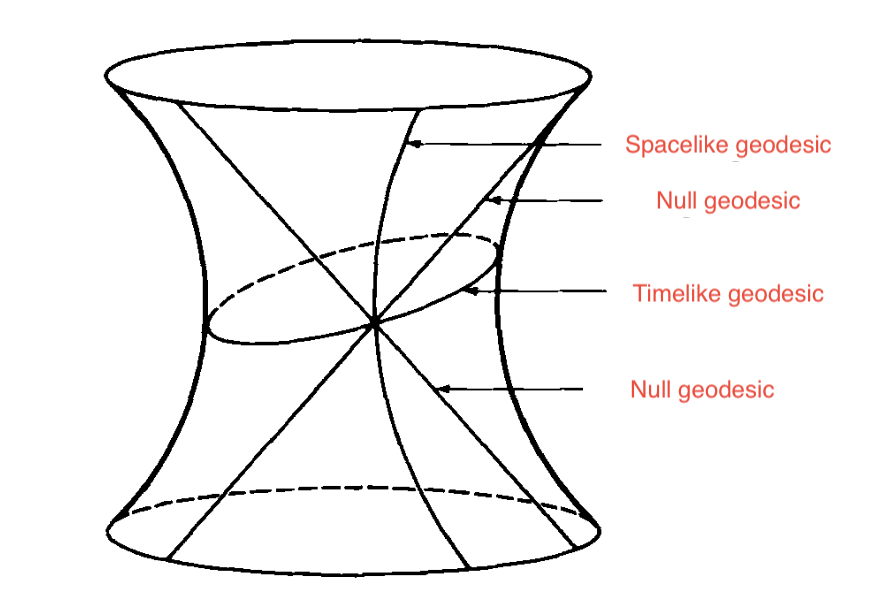
\includegraphics[width=0.7\textwidth]{Pseudospheres/geodesiques.png}
    \caption{Geodesics in the $\mathbb H^{1,1} \subseteq R^{1,2}$}
    \label{fig:geodesics_hyperbolic_plane}
\end{figure}
\begin{proposition}
    Let $q(\cdot, \cdot)$ be the metric defining the pseudohyperbolic space $\mathbb H^{n - \nu, \nu}(r)$,  $p \in \mathbb H^{n- \nu, \nu}(r)$, and $\Pi$ be a plane passing from $p$ and the origin.
    Then the intersection $\Pi \cap \mathbb H^{n - \nu, \nu}(r)$ is a geodesic in $\mathbb H^{n - \nu, \nu}(r)$, and we distinguish the following three cases:
    \begin{enumerate}[label=(\roman*)]
        \item If $\sgn(q_{|\Pi}) = (0,0,2)$, then the intersection is an ellipse, and a timelike geodesic.
        \item If $\sgn(q_{|\Pi}) = (0,1,1)$, then the intersection is a pair of parallel lines, and null geodesics.
        \item If $\sgn(q_{|\Pi}) = (1, 0, 1)$, then the intersection is a hyperbola, whose branches are spacelike geodesics.
    \end{enumerate}
    Any geodesic in $\mathbb H^{n - \nu, \nu}(r)$ is obtained as such, and in particular, the pseudohyperbolics are complete.
\end{proposition}
\begin{proof}
    \begin{enumerate}[label=(\roman*)]
        \item Let $e_1, e_2$ be an orthonormal basis for $q$ on $\Pi$, and consider the coordinates $y = (y_1, y_2)$ on $\Pi \cap \mathbb H^{n - \nu, \nu}$ such that $s = y^1(s)e_1 + y^2(s)e_2$ for $s \in \Pi \cap \mathbb H^{n - \nu, \nu}(r)$.
        Then
        \begin{align*}
            \Pi \cap \mathbb H^{n - \nu, \nu}(r) &= \left\{ y \in \mathbb R^{n - \nu, \nu + 1} : q(y,y) = -r^2 \right\}\\
            &= \left\{ y^1 e_1 + y^2 e_2 \in \mathbb R^{n - \nu, \nu + 1} : -(y^1)^2 - (y^2)^2 = -r^2 \right\},
        \end{align*}
        which is clearly an ellipse.
        It can be parametrised by $\alpha(t) = r \cos(t)e_1 + r \sin(t)e_2$ for $t \in [0, 2\pi)$, for which $\alpha'(t) = -r \sin(t) \frac{\partial}{\partial y^1} + r \cos(t) \frac{\partial}{\partial y^2}$.
        Then $\langle \alpha'(t), \alpha'(t) \rangle = -r^2$, so $\alpha$ is timelike.
        Moreover, $\tilde D_t \alpha' = - P_{\alpha(t)}$ is the opposite of the position vector, so it is normal to $\mathbb H^{n - \nu, \nu}(r)$, and hence a geodesic.
    \end{enumerate}
\end{proof}
\section{Pseudoriemannian structure}
\subsection{Pseudoriemannian structure on $\mathbb H^{p,q}$}
Since $\hat{\mathbb H}^{p,q}$ is the unit sphere in $V$ with respect to the inner product chosen, it is a manfiold whose tangent space at $x \in \hat{\mathbb H}^{p,q}$ can be identified with the orthogonal complement of $x$ in $V$:
\[
T_x \hat{\mathbb H}^{p,q} = x^\perp = \{ v \in V : \langle v, x \rangle = 0 \}.
\] 
Since every $x \in \hat{\mathbb H}^{p,q}$ is a negative vector, the metric restricted on the tangent space is of signature $(p,q)$, which makes $\hat{\mathbb H}^{p,q}$ a pseudoriemannian manifold of signature $(p,q)$.

To define a pseudoriemannian structure on 

\chapter{Linear algebra}
\section{Symplectic forms}
Recall that for a bilinear form $\omega$ on a vector space $V$, we can define the matrix $M_B(\omega)$ of $\omega$ with respect to a basis $B = (v_1, \ldots, v_n)$ of $V$ by
\[
M_B(\omega)_{ij} = \omega(v_i, v_j).
\]
In that case, the form is given by
\[
\omega\left(\sum_i x_i v_i, \sum_j y_j v_j\right) = \sum_{i,j} x_i y_j M_B(\omega)_{ij} = x^t M_B(\omega) y,
\]
where the vectors $x, y$ in the right hand side are represented by their coordinates in the basis $B$.
\begin{definition}
    Let $V$ be a complex or real vector space.
    A symplectic form $\omega: V \times V \to \R$ is a non-degenerate, skew-symmetric (i.e.\ $\omega(x,y) = - \omega(y,x)$) bilinear form.
    Equivalently, the associated matrix $M_B(\omega)$ is skew-symmetric and nonsingular.
\end{definition}
\begin{proposition}
    Every symplectic form on a finite-dimensional vector space $V$ can be written as 
    \[
    \omega = \begin{pmatrix}
        0 & I_n \\
        -I_n & 0
    \end{pmatrix}
    \]
    with respect to some basis of $V$.
\end{proposition}
\begin{proof}
    We proceed by induction on $\dim V$.
    If $\dim V = 2$, then we let $e_1$ be some non-zero vector and using non-degeneracy, we let $e_2$ be such that $\omega(e_1, e_2) = 1$.
    Then $\omega = \begin{pmatrix} 0 & 1 \\ -1 & 0 \end{pmatrix}$.
    Supposing the statement holds for $\dim V = 2n$, we consider $\dim V = 2n+2$, and using the same arguements we can find $e_1, e_2 \in V$ such that $\omega(e_1, e_2) = 1$.
    In particular, $W = \spa \{e_1, e_2\}$ is a non-degenerate subspace, so the same will be true for $W^\perp$.
    By the inductive hypothesis, we can find a basis of $W^\perp$ such that $\omega$ is given by
    \[
    \begin{pmatrix}
        0 & I_n \\
        -I_n & 0
    \end{pmatrix}.
    \]
    Then we can extend this basis to $V$ by adding $e_1, e_2$, and after rearranging the order of the basis elements, we obtain the desired form.
\end{proof}
\begin{definition}
    Let $V$ be a symplectic vector space.
    A subspace $W \subseteq V$ is called \emph{Lagrangian} if $W = W^\perp$, while a subspace $W \subseteq V$ is called \emph{isotropic} if $W \subseteq W^\perp$.
\end{definition}
\begin{proposition}
    Let $V$ be a symplectic vector space. Then:
    \begin{enumerate}[label=(\roman*)]
        \item A subspace is lagrangian subspace if and only if it is maximally isotropic.
        \item Every isotropic subspace is contained in a lagrangian subspace.
        \item Symplectic vector spaces have even-dimension. 
    \end{enumerate}
\end{proposition}
\begin{proof}
    \begin{enumerate}
        \item Let $W$ be a Lagrangian subspace and $W'$  be an isotropic subspace containing $W$.
        If $W \neq W'$, then there exists $v \in W' \setminus W$.
        Then $v \in W^\perp = W$, a contradiction.
        Letting $W$ be maximal isotropic, we have that $W \subseteq W^\perp$.
        But for every $v \in W^\perp$, we have that $\mathbb Cv + W$ is isotropic (here we use skew-symmetry of $\omega$ to obtain that $v$ is isotropic), so $v \in W$.
        That is $W = W^\perp$ and $W$ is Lagrangian.
        \item Let $W'$ be isotropic and not Lagrangian.
        Then $W$ is not maximal isotropic, that is, there exists $v \not \in W$ such that $W + \mathbb C v$ is isotropic.
        Repeating this process, we obtain an increasing chain of isotropic subspaces containing $W$, which will terminate at a Lagrangian subspace. 
        \item Using the identity
        \[
        \dim W + \dim W^\perp = \dim V
        \]
        that holds for all subspaces $W$, we obtain that $2 \dim W = \dim V$ for any lagrangian subspace $V$.
    \end{enumerate}
\end{proof}

\begin{proposition}
    Let $\omega, \omega'$ be symplectic forms on $V$.
    Then there exists a subspace $W\subseteq V$ that is Lagrangian with respect to both forms.
\end{proposition}
\begin{proof}
    Let $A = M_B(\omega') M_B(\omega)^{-1}$ with respect to some basis $B$ of $V$.
    This is exactly the matrix for which
    \[
    \omega'(v,w) = \omega(Av, w)
    \]
    Using skew-symmetry, it is easy to see that $A^* = A$ with respect to $\omega'$ (where the $*$ denotes the adjoint with respect to $\omega$).
    Then we can similarly show that it is also symmetric with respect to $\omega'$, that is:
    \[
    \omega(Av, w) = \omega(v, Aw), \omega'(Av, w) = \omega'(v, Aw).
    \]
    
    Consider the generalized eigenvalue decomposition with respect to $A$:
    \[
    V = \bigoplus_{\lambda} V_\lambda,
    \]
    where $V_\lambda = \ker\left((A - \lambda I)^{k_\lambda}\right)$ and the sum is taken over all generalized eigenvalues of $A$.
    Moreover, the following lemma implies that the decomposition is orthogonal with respect to $\omega, \omega'$.

    By counting dimensions, we see that if $W_\lambda$ is a lagrangian subspace of $V_\lambda$, then $W = \bigoplus_\lambda W_\lambda$ is a lagrangian subspace of $V$.
    Hence it suffices to consider each $V_\lambda$ separately.
    There, we may take $W_\lambda = \ker(A - \lambda I)^{k_\lambda - 1}$ and check that it is isotropic with respect to both forms.
    To do this, we proceed inductively on $\dim V_\lambda$.
    If $\dim V_\lambda = 2$, then every isotropic subspace is lagrangian, so we can take $W_\lambda$ to be the span of any vector in $V_\lambda$.
    In particular, $W_\lambda$ is lagrangian.
    If $\dim V_\lambda = 2n$, then the quotient space $W_\lambda^\perp / W_\lambda$ is symplectic and by the inductive hypothesis, there exist $v_1, \cdots, v_r \in W^\perp - W$ such that $W + \mathbb C v_1 \oplus \cdots \oplus W + \mathbb C v_r$ is lagrangian.
    Then $W \oplus \mathbb C v_1 + \cdots \oplus \mathbb C v_r$ is isotropic and by dimension counting, we see it is lagrangian as well.
\end{proof}
\begin{lemma}
    Let $V$ be a vector space with bilinear form $\omega$.
    Then every matrix $A$ that is self-adjoint with respect to $\omega$ has orthogonal generalized eigenspaces.
\end{lemma}
\begin{proof}
    Let $u \in V_\lambda, v \in V_\mu$ and consider polynomials $P(x) = (x - \lambda)^{k_\lambda}, Q(x) = (x - \mu)^{k_\mu}$.
    Then $P, Q$ are prime with each other, so there exist polynomials $U, V$ such that $UP + VQ = 1$.
    Then $\omega(u,v) = \omega((UP + VQ)(A)u, v) = \omega(VQ(A)u, v) = \omega(u, VQ(A)v) = 0 $, where we use that since $P(A),Q(A)$ are polynomials of $A$, they are self-adjoint as well.
\end{proof}

\section{Proximal elements in $\GL(n,\R)$}
Here we will talk about basic definitions and dynamics of proximal elements in $\GL(n,\R)$ and its subgroups.
\begin{definition}
    We say that $g \in \PGL(d, \mathbb R)$ is \emph{proximal} (in $\mathbb P(\mathbb R^d)$) if it admits an attractive fixed point in $\mathbb P(\mathbb R^d)$, i.e. there exists a line $x_g^+ \in \mathbb P(\mathbb R^d)$ and a compact neighborhood $b^+ \subseteq \mathbb P(\mathbb R^d)$ of $x+g^+$ such that $g^n x \to x $ as $n \to \infty$ uniformly for $x \in b^+$.
    We say that $g$ is biproximal if both $g$ and $g^{-1}$ are proximal.
\end{definition}

To better understand the dynamics of proximal elements, we will recall the Jordan decomposition of a matrix.
Let $A \in \GL(d,\mathbb R)$.
Then $A$ admits a Jordan canonical form $A = B J B^{-1}$, where $B \in \GL(d, \mathbb R)$ and $J$ is a block diagonal matrix with Jordan blocks $J_1, \ldots, J_k$:
\[
J = \begin{pmatrix}
    J_1 & & \\
    & \ddots & \\
    & & J_m
\end{pmatrix},
\]
where each $J_i$ is either a single real entry $j_i$, or a (real) Jordan block of the form
\[
J_i = \begin{pmatrix}
    C_i & 1 & & \\
    & C_i & \ddots & \\
    & & \ddots & 1 \\
    & & & C_i
\end{pmatrix},
\]
with $C_i$ being a $2 \times 2$ matrix of the form
\[
C_i = \begin{pmatrix}
    a_i & -b_i \\
    b_i & a_i
\end{pmatrix},
\]
and $b_i \neq 0$.
In the latter case, we let $j_i$ be one of the complex eigenvalues $j_i = \sqrt{\det C_i} e^{i \arccos(a_i)}$ of $C_i$.
\begin{remark}
    Each $C_i$ is merely a similitude (in case $C_i$ is not a single entry) by $|j_i| = \sqrt{\det C_i}$ of a rotation by $\arccos a_i$, so $J_i$ rotates and multiplies the plane corresponding to its first two collumns.
\end{remark}
We call each $j_i$ a \emph{generalised eigenvalue} of $A$ and the subspace $E_i$ preserved by each $J_i$ the \emph{generalised eigenspace} of $j_i$.
By changing $B$ we may assume that $|j_1| \geq \ldots \geq |j_m|$.

We are now ready to describe the dynamics of a Jordan block, which is the same as the dynamics of $A$ in the respective generalised eigenspace.
\begin{lemma}[Dynamics of a Jordan block]
    Let $J_i$ be a Jordan block, and let $j_i, E_i$ be its generalised eigenvalue and eigenspace respectively.
    We denote with $e_1, \cdots, e_k$ part of the standard basis that spans $E_i$.
    \begin{enumerate}[label=(\roman*)]
        \item There exists vectors $v \in E_i$ such that
        \[
        |J_i^n v| = |j_i|^n |v|.
        \]
        When $C_i$ is a real entry, this holds for $v \in \mathbb Rv_1$, while when $C_i$ is a $2 \times 2$ matrix, this holds for $v \in \mathbb R e_1 \oplus \mathbb R e_2$.
        \item If $J_i$ is upper-triangular but not a single entry, then $E_i$ contains an actual eigenvector (namely $e_1$) such that for $v \in E_i$ we have $J_i^n \mathbb Rv \to \mathbb Re_1$.
        \item If $J_i$ is not upper-triangular, then the generalized eigenspace $E_i$ contains no eigenvalues, and there exists no attracting point in $\mathbb P(E_i)$.
        \item If $J_i$ is upper-triangular but not a single entry, then the convergence in the eigenspace $E_i$ is not uniform.
        \item A Jordan matrix $J$ is proximal if and only if $|j_1| > |j_2|$ and $J_1$ is a real entry.
    \end{enumerate}
    \begin{proof}
        While we will not give a concrete proof of this fact, we can consider examples.
        \begin{enumerate}[label=(\roman*)]
            \item This follows by the fact that for $v$ in the respective subspaces, $J_i$ is a similitude by $j_i$ and perhaps a rotation.
            \item 
            Suppose $J$ is $2\times 2$, so
            \[
            J_i = \begin{pmatrix}
                a_i & 1 \\
                0 & a_i
            \end{pmatrix}.
            \]
            Let $w \in E_2$, we can write $\mathbb R w = \mathbb R(w_1 e_1 + e_2)$.
            Inductively we show that 
            \[
            J_i^n \mathbb R w = \mathbb R((w_1 j + n)e_1 + j e_2),
            \]
            which clearly converges to $\mathbb R e_1$ as $n \to \infty$.
            \item It is clear that $\mathbb P(E_i)$ contains no eigenvalues.
            To see that it contains no attracting fixed points, assume that $J_i$ is $2\times 2$.
            Then $J_i$ acts on $\mathbb R e_1 \oplus \mathbb R e_2$ as a rotation and a similitude by, so any point line there does not converge.
            \item Let 
            \[
            J = \begin{pmatrix}
                j & 1 \\
                0 & j
            \end{pmatrix} \text{ and } v_n = (n, -j).
            \]
            Then 
            \[
            J^n = \begin{pmatrix}
                j & n\\
                0 & j
                \end{pmatrix} \text{ in } \PGL(2, \mathbb R), \text{ and } J^n \mathbb R v_n = \begin{pmatrix}
                    0\\
                    -1
                \end{pmatrix}.
            \]
            \item If $|j_1| > |j_2|$ and $J_1$ is a real entry, then for $w \in \mathbb R^d$, we can write $w = w_1 + \cdots + w_m$ with each $w_i \in E_i$.
            Then in the projective space, we have
            \[
            J^n w = \frac{1}{|j_1|^n} J_1 w_1 + \cdots + \frac{1}{|j_1|^n} J_m w_m,
            \]
            with
            \[
            |\frac{1}{|j_1|^n} J^n w_i| = \left(\frac{j_i}{j_1}\right)^n |w_i| \to 0 \text{ for } i \geq 2 \text{ uniformly on compact sets.}
            \]
            So $J^n w \to \mathbb R e_1$ uniformly on compact neighborhoods of $\mathbb R e_1$.
            If on the other hand $|j_1| = |j_2|$, then the same arguement shows that $J^n$ does not converge for $w \in E_1 \oplus E_2$, while for $|j_1| > |j_2|$, not being a single entry means that either there is no attractive fixed point or that the convergence is not uniform.
        \end{enumerate}
    \end{proof}
\end{lemma}

We now consider the Jordan matrix (see \cref{fig:jordan_matrix_dynamics}):
\begin{proposition}[Dynamics of a Jordan matrix]
    Let $J$ be a Jordan matrix with Jordan blocks $J_1, \cdots J_m$.
    Then $J$ is proximal if and only if $|j_1| > |j_2|$ and $ J_1$ is a real entry.
    In that case, for any $x \in \spa \{e_2, \cdots, e_d \}^c$ we have
    \[
    J^n x \to \mathbb R e_1,
    \]
    and the convergence is uniform in compact neighborhoods of $\spa \{e_2, \cdots, e_d \}^c$.
    Similarly, $J$ is biproximal if and only if $|j_1| > |j_2|, |j_{m-1}| > |j_m|$ and $J_1, J_m$ are real entries.
    In that case, for any $x \in \spa \{e_1, \cdots, e_{d-1} \}^c$ we have
    \[
    J^{-n} x \to \mathbb R e_d,
    \]
    and the convergence is uniform in compact neighborhoods of $\spa \{e_1, \cdots, e_{d-1} \}^c$.
\end{proposition}
\begin{proof}
    Note that if $|j_1| > |j_2|$ and $J_1$ is a real entry, then for $w \not \in \spa{ e_2, \cdots, e_d}$, we can write $w = w_1 + \cdots + w_m$ with each $w_i \in E_i$.
    Then 
    \[
    J^n \mathbb R w = \mathbb R (J_1^n w_1 + \cdots + J_m^n w_m) = 
    \mathbb R (w_1 + \frac{J_2^n}{j_1^n} w_2 + \cdots + \frac{J_m^n}{j_1^n} w_m) \to \mathbb R e_1,
    \]
    where the last convergence holds since each of the eigenvalues $j_i$ are less than $j_1$.

    If on the other hand $J$ is proximal, we have seen that in the remark above, that $J_1$ needs to be a single entry, otherwise the convergence is not uniform.
    On the other hand, if $|j_1| = |j_2|$, then $J$ will rotate the plane spanned by $e_2, e_3$, like for instance when
    \[
    J = \begin{pmatrix}
        1 & 0 & 0 \\
        0 & \cos \theta & - \sin \theta \\
        0 & \sin \theta & \cos \theta
    \end{pmatrix}, v = (1, x, y), J^n v = \begin{pmatrix}
        1\\
        \begin{pmatrix}
            \cos n \theta & - \sin n \theta \\
            \sin n \theta & \cos n \theta
        \end{pmatrix}
        \begin{pmatrix}
            x \\ y
        \end{pmatrix}
    \end{pmatrix}
    \]
\end{proof}
\begin{figure}[ht]
    \centering
    \begin{subfigure}[b]{0.45\textwidth}
        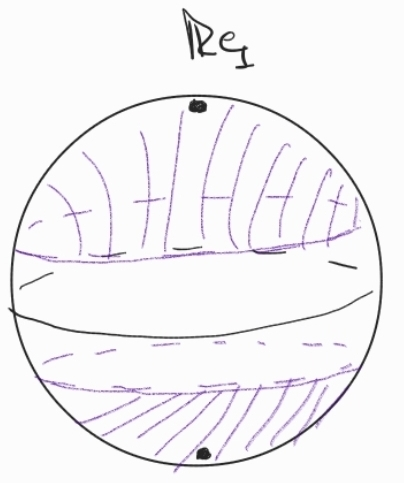
\includegraphics[width=\textwidth]{jordan_dynamics3}
        \caption{In the double cover $S^2$ convergence is uniform when uniformly away from the equator.}
        \label{fig:jordan_dynamics_sphere}
    \end{subfigure}
    \hfill
    \begin{subfigure}[b]{0.45\textwidth}
        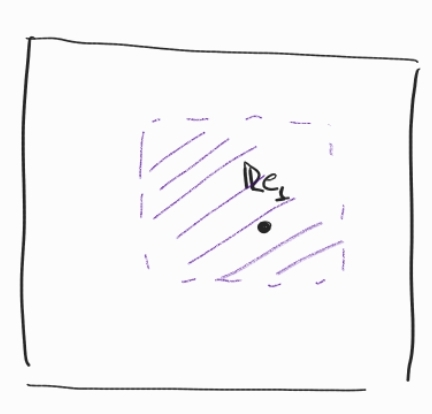
\includegraphics[width=\textwidth]{jordan_dynamics2}
        \caption{In the affine chart $\mathbb R^2 \simeq \{ [1, x, y] \}$, convergence is uniform when uniformly away from the circle at infinity.}
        \label{fig:jordan_dynamics_affine_chart}
    \end{subfigure}
    \caption{Dynamics of Jordan matrix on $\mathbb P(\mathbb R^3)$}
    \label{fig:jordan_matrix_dynamics}
\end{figure}
Noting that being proximal is invariant under conjugation, we can now describe the dynamics of a proximal element in $\GL(d, \mathbb R)$:
\begin{corollary}
    Let $g \in \PGL(d, \mathbb R)$ and denote with $g$ any of its representatives.
    Then the following are equivalent:
    \begin{enumerate}[label=(\roman*)]
        \item $g$ is proximal if and only if $g$ has a Jordan decomposition $g = B J B^{-1}$ with $J$ being proximal.
        \item Denoting with $\lambda_1(g), \cdots \lambda_d(g)$ the (possibly complex) eigenvalues of $g$ in decreasing order of their modulus, $g$ is proximal if and only if $|\lambda_1(g)| > |\lambda_2(g)|$.
    \end{enumerate}
    and similarly for biproximal elements:
    \begin{enumerate}[label=(\roman*)]
        \item $g$ is biproximal if and only if $g$ has a Jordan decomposition $g = B J B^{-1}$ with $J$ being biproximal.
        \item Denoting with $\lambda_1(g), \cdots \lambda_d(g)$ the (possibly complex) eigenvalues of $g$ in decreasing order of their modulus, $g$ is proximal if and only if $|\lambda_1(g)| > |\lambda_2(g)|$ and $|\lambda_{d-1}(g)| > |\lambda_d(g)|$.
    \end{enumerate}
    If this is the case, the attracting fixed point of $g$ is the line spanned by the eigenvector $Be_1$ and the convergence is uniform in compact neighborhoods of $\spa \{Be_2, \cdots, Be_d \}^c$.
\end{corollary}

Considering the case of $\PO(p, q)$ for $p, q \geq 0$, we have that every proximal element is biproximal:
\begin{proposition}
    In $\PO(p, q)$, proximality and biproximality are equivalent.
\end{proposition}
\begin{proof}
    Let $g \in \PO(p, q)$ be proximal.
    Then the eigenvalues of $g$ are stable under taking inverse: $\lambda(g) = \lambda(g^{-1})$.
    Indeed, $g \in \OO(p,q)$ implies that $g^t I_{p,q} g = I_{p,q}$, so for an eigenvector $v$ of $g$ with eigenvalue $\lambda$, we multiply $gv = \lambda v$ by $I_{p,q}$ to obtain that 
    \[
    \lambda I_{p,q} v =I_{p,q} g v = (g^t)^{-1} I_{p,q} v,
    \]
    so $\sigma(g) \subseteq \sigma((g^t)^{-1}) = \sigma(g^{-1})$.
\end{proof}
%%%%%%%%%%%%%%%%%%%%%%%%%%%%%%%%%%%%%%%%%%%%%%%%%
\section{Complexification of vector spaces}
\begin{definition}
    Let $V$ be a real vector space and $\rho: \mathfrak g \to \mathfrak{gl}(V)$ a representation of a real Lie algebra $\mathfrak g$.
    \begin{enumerate}[label=(\roman*)]
        \item The complexification $V^\mathbb C$ of $V$ is the complex vector space defined setwise by $V \times V$, with the addition structure of $V \oplus V$ and the scalar multiplication rule $(x + i y) (v_1, v_2) = (x v_1 - y v_2, x v_2 + y v_1)$.
        We write $(v_1, v_2)$ as $v_1 + i v_2$.
        \item If $W$ is a complex vector space isomorphic to the complexification of $V$, then we say that $V$ is a real form of $W$.
    \end{enumerate}
\end{definition}

Recall that a map $f: V \to V$ on a complex vector space $V$ is called \emph{antilinear} if it it satisfies $f(u + v) = f(u) + f(v)$ and $f(\lambda v) = \overline \lambda f(v)$.
\begin{definition}
    Let $V$ be a complex vector space.
    A conjugation on $V$ is an antilinear map $C: V \to V$ such that $C^2 = \id$.
\end{definition}
\begin{example}
    If $E$ is a real vector space and $V= E^\mathbb C$, then we can define the conjugation $C: V \to V$ by $C(v) = \overline v$, where $\overline{u + iv} = u - iv$.
\end{example}
\begin{proposition}
    Let $V$ be a complex vector space.
    Then real forms of $V$ are in bijective correspondence with conjugations on $V$.
\end{proposition}
\begin{proof}
    To each real form $E$ of $V$, we can associate the conjugation $C(u + iv) = u - iv$, for $u, v \in E$.
    Conversely, for each conjugation $C$ on $V$, we consider the real vector space $E = \{ v \in V \mid C(v) = v \}$, which turns out to be a real form of $V$.
\end{proof}

\begin{proposition}
    If $\mathfrak E$ is a representation of $\mathfrak g$ that is not of real type, then there exists an irreducible complex representation $V \subseteq E^\mathbb C$ of $\mathfrak g^\mathbb C$, such that
    \[
    E^\mathbb C = V \oplus \overline V,
    \]
    whre $\overline V$ is the conjugate representation of $V$, i.e. $\overline V = \{ \overline v \mid v \in V \}$ and the action of $\mathfrak g$ on $\overline V$ is given by $\rho(X)(\overline v) = \overline{\rho(X)v}$.
\end{proposition}
\begin{proof}
    Let $V$ be a complex subspace of $E^\mathbb C$ that is invariant under $\mathfrak g^\mathbb C$.
    Then $\overline V$ is also invariant under $\mathfrak g^\mathbb C$, so the same is true for $V \cap \overline V$ and $V + \overline V$.
    Since these are invariant under the conjugation of $E^\mathbb C$, we have that $V + \overline V, V \cap \overline V$ admit real forms.
    Moreover, because the action of $\mathfrak g^\mathbb C$ commutes with conjugation,the real forms are invariant under the action of $\mathfrak g$.
    By irreducibility of $E$, we obtain that $V \oplus \overline V = E^\mathbb C$.
\end{proof}
\chapter{Riemannian calculations}
\section{Sphere}
\subsection{Round metric on the sphere}
\todo{Do the same for stereographic coordinates, see whether it is possible to obtain it in different coordinates directly through the euclidean metric, generalize to higher dimensions.}
    On the sphere of radious $R$, the round metric is defined as the metric induced by the Euclidean metric of $\mathbb R^{n+1}$.
    Recall that the spherical coordinates on $\mathbb S^n$ are given by
    \begin{align*}
        \phi^{-1}: (0,2\pi) \times (0,\pi) &\to \mathbb S^2\\
        (\theta, \varphi) &\mapsto (R \cos \theta \sin \varphi, R \sin \theta \sin \varphi, R \cos \varphi).
    \end{align*}
    In these coordinates, the round metric is given by
    \[
    g = R^2 (\sin^2 \varphi d\theta^2 + d\varphi^2).
    \]
    \begin{proof}
        We compute the frame given by the coordinate vector fields:
        \begin{align*}
            \frac{\partial}{\partial \theta} &= -R \sin \theta \sin \varphi \frac{\partial}{\partial r^1} + R \cos \theta \sin \varphi \frac{\partial}{\partial r^2}  \\
            \frac{\partial}{\partial \varphi} &= R \cos \theta \cos \varphi \frac{\partial}{\partial r^1} + R \sin \theta \cos \varphi \frac{\partial}{\partial r^2} - R \sin \varphi \frac{\partial}{\partial r^3}.
        \end{align*}
        Then we compute the coefficients using the Euclidean metric of $\mathbb R^3$:
    \begin{align*}
        g_{\theta \theta} &= \left\langle \frac{\partial}{\partial \theta}, \frac{\partial}{\partial \theta} \right\rangle = R^2 \sin^2 \varphi\\
        g_{\varphi \varphi} &= \left\langle \frac{\partial}{\partial \varphi}, \frac{\partial}{\partial \varphi} \right\rangle = R^2\\
        g_{\theta \varphi} &= \left\langle \frac{\partial}{\partial \theta}, \frac{\partial}{\partial \varphi} \right\rangle = 0.
    \end{align*}
    \end{proof}
\subsection{Volume form on the sphere}
We will compute the volume form of the round metric on $\mathbb S^2$ in spherical coordinates.
We saw that in these coordinates, the round metric in matrix form is
\[
g = R^2 \begin{pmatrix}
\sin^2 \varphi & 0 \\
0 & 1
\end{pmatrix}.
\]
Hence the volume form is simply
\[
\text{Vol} = \sqrt{\det g} d\theta d\varphi = R^2 \sin \varphi \d\theta \wedge \d\varphi.
\]
\todo{Volume entropy}

\subsection{Hyperbolic space}
\subsubsection{Coordinate representation for metric}
    We consider the hyperboloid model of the hyperbolic space $\mathbb H^n$:
    \[
    \mathbb H^n = \{x \in \mathbb R^{n,1}: x_1^2 + \cdots + x_n^2 - x_{n+1}^2 = -1, x_{n+1} > 0\},
    \]
    with the metric induced by the Minkowski metric of $\mathbb R^{n,1}$.
    
    \begin{proposition}[Coordinates for projection chart]
        Consider the chart that projects the hyperboloid onto the plane $x_{3} = 0$:
        \begin{align*}
            \phi = (u,v): \mathbb H^2 &\to \mathbb R^2\\
            (r^1, r^2, r^3) &\mapsto (r^1, r^2).
        \end{align*}
    In these coordinates, the hyperbolic metric is given by
    \[
    g = \frac{(1 + v^2) du^2 + (1 + u^2) dv^2 - uv du dv}{1 + u^2 + v^2},
    \]
    where $du dv$ is the symmetric product $\frac{1}{2}(du \otimes dv + dv \otimes du)$.
    \end{proposition}
    \begin{proof}
    The parametrization we use is given by
    \begin{align*}
        \phi^{-1}: \mathbb R^2 &\to \mathbb H^2\\
        (u,v) &\mapsto (u, v, \sqrt{1 + u^2 + v^2}).
    \end{align*}
    
        We compute the frame given by the coordinate vector fields:
        \begin{align*}
            \frac{\partial}{\partial u} &= \frac{\partial}{\partial r^1} + \frac{u}{\sqrt{1 + u^2 + v^2}} \frac{\partial}{\partial r^3}\\
            \frac{\partial}{\partial v} &= \frac{\partial}{\partial r^2} + \frac{v}{\sqrt{1 + u^2 + v^2}} \frac{\partial}{\partial r^3}.
        \end{align*}
        Then we compute the coefficients using the Minkowski metric of $\mathbb R^{2,1}$:
    \begin{align*}
        g_{uu} &= \left\langle \frac{\partial}{\partial u}, \frac{\partial}{\partial u} \right\rangle = 1 - \frac{u^2}{1 + u^2 + v^2} = \frac{1 + v^2}{1 + u^2 + v^2}\\
        g_{vv} &= \left\langle \frac{\partial}{\partial v}, \frac{\partial}{\partial v} \right\rangle = 1 - \frac{v^2}{1 + u^2 + v^2} = \frac{1 + u^2}{1 + u^2 + v^2}\\
        g_{uv} &= \left\langle \frac{\partial}{\partial u}, \frac{\partial}{\partial v} \right\rangle = - \frac{uv}{1 + u^2 + v^2}.
    \end{align*}
    Thus the metric is given by
    \[
    g = \frac{(1 + v^2) du^2 + (1 + u^2) dv^2 - uv du dv}{1 + u^2 + v^2}.
    \]
    \end{proof}\todo{Inherited metric from projective space is the same with identifying tangent space with orthogonal complement?}

    \begin{proposition}[Geodesic polar coordinates]
        In geodesic polar coordinates, the hyperbolic metric is given by
        \[
        g = \d r^2 + \sinh^2(r) \d\theta^2.
        \]
    \end{proposition}
    \begin{proof}
        Without loss of generality, we can assume that the point we are considering is $p = (0,0,1)$.
        First we calculate the exponential map at $p$:
        \begin{align*}
            \exp_p: T_p \mathbb H^2 &\to \mathbb H^2\\
            v_1 \frac{\partial}{\partial r^1} + v_2 \frac{\partial}{\partial r^2} &\mapsto \left(\cosh(\|v\|), \sinh(\|v\|) \frac{v}{\|v\|}\right),
        \end{align*}
        where $\|v_1 \partial_{r^1} + \cdots + v_3 \partial_{r^3}\| = \sqrt{(v_1)^2 + (v_2)^2 + (v_3)^2}$ is the usual euclidean norm.

        Then we identify the tangent space $T_p \mathbb H^2$ with $\mathbb R^2$, via $v_1 \partial_{r^1} + v_2 \partial_{r^2} \mapsto (v_1, v_2)$, and compose with the polar coordinates of $\mathbb R^2 - \{0\}$ so we obtain the commutative diagram
        \[
            \begin{tikzcd}
                \mathbb R^2 \simeq T_p \mathbb H^2  \arrow[r, "\exp_p"] & \mathbb H^2\\
                \mathbb R_{>0} \times (0, 2\pi) \arrow[u, "\phi^{-1}"] \arrow[ur, "\phi^{-1} \circ \exp_p"]
            \end{tikzcd}
        \]
        where $\phi$ is the chart of geodesic polar coordinates:
        \begin{align*}
            \phi^{-1}: \mathbb R_{>0} \times (0, 2\pi) &\to \mathbb H^2\\
            (r, \theta) &\mapsto (\sinh(r) \cos(\theta), \sinh(r) \sin(\theta), \cosh(r)).
        \end{align*}
        Then we compute the frame given by the coordinate vector fields with respect to the ambient coordinates of $\mathbb R^{2,1}$:
        \begin{align*}
            \frac{\partial}{\partial r} &= \cosh(r) \cos(\theta) \frac{\partial}{\partial x^1} + \cosh(r) \sin(\theta) \frac{\partial}{\partial x^2} + \sinh(r) \frac{\partial}{\partial x^3}\\
            \frac{\partial}{\partial \theta} &= -\sinh(r) \sin(\theta) \frac{\partial}{\partial x^1} + \sinh(r) \cos(\theta) \frac{\partial}{\partial x^2}.
        \end{align*}
        Then we compute the coefficients using the metric in the ambient coordinates given by the Minkowski metric of $\mathbb R^{2,1}$:
    \begin{align*}
        g_{rr} &= \left\langle \frac{\partial}{\partial r}, \frac{\partial}{\partial r} \right\rangle = 1\\
        g_{\theta \theta} &= \left\langle \frac{\partial}{\partial \theta}, \frac{\partial}{\partial \theta} \right\rangle = \sinh^2(r)\\
        g_{r \theta} &= \left\langle \frac{\partial}{\partial r}, \frac{\partial}{\partial \theta} \right\rangle = 0,
    \end{align*}
    and the result follows.
    \end{proof}

\subsection{Projective space} 
Round metric in projective space:\\
    We consider the projective space $\mathbb P(\mathbb R^{n+1})$ with the round metric, i.e.\ the metric induced by the round metric of the sphere $\mathbb S^n \subseteq \mathbb R^{n+1}$ through the double covering $\pi: \mathbb S^n \to \mathbb P(\mathbb R^{n+1})$.
    We use the affine chart $U_3 = \{[x:y:z] \in \mathbb P(\mathbb R^3): z \neq 0\} \simeq \mathbb R^2$:
    \begin{align*}
        \phi^{-1}: \mathbb R^n &\to U_3 \subseteq \mathbb P(\mathbb R^3)\\
        (u,v) &\mapsto [u:v:1].
    \end{align*}
    In these coordinates, the round metric is given by
    \[
    g = \frac{(1 + v^2) du^2 + (1 + u^2) dv^2 - uv du dv}{(1 + u^2 + v^2)^2},
    \]
    \begin{proof}
        Note that for instance to compute $g_{uu}$, what we need is to compute the norm of $(\d \pi)^{-1}(\partial/\partial u)$ in the round metric of $\mathbb S^2$, since the metric on $\mathbb P(\mathbb R^3)$ is defined as the pullback of the metric on $\mathbb S^2$ through $\pi^{-1}$ (in a neighborhood where $\pi$ is invertible).
        For this reason, we limit ourselves too the restriction $\pi^{-1}: U_3 \to \mathbb U_N$, where $\mathbb U_N$ is chart of the upper hemisphere.
        Then indeed,
        \[
        g_{uu} = g\left(\frac{\partial}{\partial u}, \frac{\partial}{\partial u}\right) = 
        \left\langle (\d \pi)^{-1}\left(\frac{\partial}{\partial u}\right), (\d \pi)^{-1}\left(\frac{\partial}{\partial u}\right) \right\rangle_{\mathbb S^2}.
        \]
        Now we compute the images of the coordinate vector fields:
        \begin{align*}
            (\d \pi)^{-1}\left(\frac{\partial}{\partial u}\right) &= \frac{1}{(1+ u^2 + v^2)^{3/2}} \left((1 + v^2) \frac{\partial}{\partial X} - uv \frac{\partial}{\partial Y} - u \frac{\partial}{\partial Z}\right)\\
            (\d \pi)^{-1}\left(\frac{\partial}{\partial v}\right) &= \frac{1}{(1+ u^2 + v^2)^{3/2}} \left(-uv \frac{\partial}{\partial X} + (1 + u^2) \frac{\partial}{\partial Y} - v \frac{\partial}{\partial Z}\right),
        \end{align*}
        where $(X,Y,Z): U_N \to \mathbb B^2$ is the chart of the upper hemisphere.
        Then we compute the coefficients using the round metric of $\mathbb S^2$, which is no other than the Euclidean metric of $\mathbb R^3$ restricted to $\mathbb S^2$:
    \begin{align*}
        g_{uu} &= \left\langle (\d \pi)^{-1}\left(\frac{\partial}{\partial u}\right), (\d \pi)^{-1}\left(\frac{\partial}{\partial u}\right) \right\rangle_{\mathbb S^2} = \frac{1 + v^2}{(1 + u^2 + v^2)^2}\\
        g_{vv} &= \left\langle (\d \pi)^{-1}\left(\frac{\partial}{\partial v}\right), (\d \pi)^{-1}\left(\frac{\partial}{\partial v}\right) \right\rangle_{\mathbb S^2} = \frac{1 + u^2}{(1 + u^2 + v^2)^2}\\
        g_{uv} &= \left\langle (\d \pi)^{-1}\left(\frac{\partial}{\partial u}\right), (\d \pi)^{-1}\left(\frac{\partial}{\partial v}\right) \right\rangle_{\mathbb S^2} = - \frac{uv}{(1 + u^2 + v^2)^2}.
    \end{align*}
    Thus the metric is given by
    \[
    g = \frac{(1 + v^2) du^2 + (1 + u^2) dv^2 - uv du dv}{(1 + u^2 + v^2)^2}.
    \]
    \end{proof}
    \todo{Projective space: Fubini-Study, Hilbert, round/symmetric metrics}

\chapter{Logbook}
\setcounter{secnumdepth}{0}
\section{2025-02-19}
\begin{itemize}
    \item Consider the irreducible subrepresentation of the symmetric square of the standard representation of $\SO(p,1)$.
    It takes values in $\SO\left(\frac{p(p-1)}{2}, p\right)$:
    \[
    \rho = \Sym^2 \mathrm{std}: \SO(p,1) \to \SO\left(\frac{p(p-1)}{2}, p\right)
    \]
    \begin{proof}
        Denoting with $\omega(u,v) = u_1 v_1 + \cdots + u_p v_p - u_{p+1}v_{p+1}$ the form preserved by $\SO(p,1)$, we can use it to identify $\Sym^2(\R^{p+1})$ with the space of symmetric forms on $\R^{p+1}$.
        Then the fact that the standard representation preserves $\omega$ is equivalent to the symmetric square preserving $\omega$ as an element of $\Sym^2{\mathbb R^{p+1}}$.
        Moreover, the symmetric square preserves $\Sym^2 \omega$, so it preserves the orthogonal complement of $\mathbb R \omega$ with respect to $\Sym^2 \omega$, which we denote with $\Sym^2_0 \mathbb R^{p+1}$.
        Using the Weyl character formula, one can show that $\rho: \SO(p,1) \to \SO(\Sym^2_0 \mathbb R^{p+1})$ is irreducible.
        Also, the signature of $\Sym^2 \omega$ on $\Sym^2 \mathbb R^{p+1}$ is $\left(\frac{p(p-1)}{2} + 1, p\right)$, and $\omega$ is positive for $\Sym^2 \omega$.
    \end{proof}
    \item Let $\Gamma \subseteq \SO(p,1)$ be a uniform lattice. Then
    $\rho: \Gamma \to \SL(\Sym_0^2(\mathbb R^{p+1}))$ is $P_1$-Anosov.
    \begin{proof}
        Consider the compact subgroup $K = \SO(p)$ of $\SO(p,1)$ (block diagonal matrices with a matrix of $\SO(p)$ for the first block and $1$ for the second block).
        Then $\rho(K) \subseteq K'$ for some compact subgroup $K'$ of $\SL(\Sym^2_0 \mathbb R^{p+1})$.
        For $A$ and $A'$ being the diagonal matrices of $\SO(p,1)$ and $\SL(\Sym^2_0 \mathbb R^{p+1})$ respectively, we have $\rho(A) \subseteq A'$.
        Writing the Cartan decomposition $g = k e^{\mu(g)} l$ of some $g \in \SO(p,1)$, we have that $\rho(g) = \rho(k) e^{\rho_* \mu(g)} \rho(l)$, so $\mu(\rho(g)) = \rho_*(\mu(g))$.
        Since $\rho: \SO(p,1) \to \GL(\Sym^2_0 \mathbb R^{p+1})$ is the irreducible representation of $\SO(p,1)$ whose complexification is the one having the highest weight $2L_1$, we know that $\rho_*(\mu(g))$ is the diagonal matrix whose diagonal entries are the weights of $\rho$ evaluated at $\mu(g)$.
        In particular, the two highest weights are $2L_1$ and $L_1 + L_2$ (the latter being equal to $L_1$ for $g \in \SO(p,1)$).
        Hence $\alpha_{12}(\rho_*(\mu(g))) = L_1(\mu(g))$.
        Since $\SO(p,1) = \Isom(H^p)$ is of rank $1$, there exists a constant $C$ such that $L_1 = d(- \cdot o, o) \mathfrak a^*$,
        where $o = e^{p+1}$ is the basepoint of $H^p$ for which $K = \Stab(o)$.
        
        On the other hand $\Gamma$ is a uniform lattice of $\Isom(\mathbb H^p)$, so the action of $\Gamma$ on $\mathbb H^p$ is cocompact and properly discontinuous.
        By the lemma of Milnor-Svarc, the map $\gamma \mapsto \gamma \cdot o$ is a quasi-isometry, meaning that $\mu(\rho(g)) = Cd(\gamma \cdot o, o ) \geq C|\gamma| - c$ for some $C, c > 0$.
    \end{proof}
    \item Calculation of the limit map $\xi: \partial \mathbb H^p \to \mathbb P(\mathbb R^d)$.
    Here we use the following description of the algebra $\sso(p,1) = \{x \in \mathfrak sl(p+1, \mathbb R): x^t M + M x = 0\}$, where 
    \[
    M = \begin{pmatrix}
        0 & \cdots & 1 \\
        \vdots & I_{p-1} & \vdots\\
        1 & \cdots & 0
    \end{pmatrix}.
    \]
    In matrix form:
    \[
    \sso(p,1) = \left\{
        \begin{pmatrix}
            X_{11} & X_{12} & 0 \\
            X_{21} & X_{22} & -X_{12}^t \\
            0 & -X_{21}^t & -X_{11}^t
        \end{pmatrix}:
        \begin{array}{c}
            X_{11} \in \mathbb R, X_{12} \in \mathbb R^{1 \times (p-1)}, X_{21} \in \mathbb R^{(p-1) \times 1}, X_{22} \in \mathbb R^{(p-1) \times (p-1)}, \\
            X_{22}^t = -X_{22}
        \end{array}
    \right\}.
    \]

    Fixing $x_0 = [e_{p+1}] \in \partial \mathbb H_\infty^p$, we have 
    \[
    \mathfrak p_0 = \mathrm{St}_{\mathfrak{so}(p,1)}(\mathbb R e_{p+1}) = \left\{ 
        \begin{pmatrix}
            -t & 0 & 0 \\
            X_{21} & X_{22} & 0 \\
            0 & -X_{21}^t & t
        \end{pmatrix} : 
        \begin{array}{c}
            t \in \mathbb R, X_{12} \in \mathbb R^{1 \times (p-1)}, X_{21} \in \mathbb R^{(p-1) \times 1}, X_{22} \in \mathbb R^{(p-1) \times (p-1)}, \\
            X_{22}^t = -X_{22}
        \end{array}
     \right\}.
    \]
\end{itemize}
\section{2025-02-21}
\begin{itemize}
    \item $\PSL(2,\mathbb R)$ is isomorphic to the group of orientation-preserving isometries of the hyperbolic plane:
    \[
    \PSL(2,\mathbb R) \simeq \SO_0(2,1)
    \]
    In fact, the isomorphism is given by the symmetric square of the standard representation of $\SL(2,\mathbb R)$.
    \begin{proof}
        Consider the symmetric square $\rho = \Sym^2 \mathrm{std}: \SL(2,\mathbb R) \to \GL(\Sym^2(\mathbb R))$ of the standard representation of $\SL(2,\mathbb R)$.
        Since the standard representation preserves the determinant, the symmetric square preserves the form $\omega = -\Sym^2\det$, which can be found to be of signature $(2,1)$.
        We have thus a representation $\rho: \SL(2,\mathbb R) \to \SO(2,1)$.
        Since $\SO(2,\mathbb R)$ is connected, we have that $\rho(\SL(2,\mathbb R)) \subseteq \SO_0(2,1)$.
        Moreover, looking at the action of $\SL(2,\mathbb R)$ on the space of symmetric $2$-tensors, we see that $\rho$ factors through $\PSL(2,\mathbb R)$.
        Since $\PSL(2,\mathbb R)$ is simple, $\rho:\PSL(2,\mathbb R) \to \SO_0(2,1)$ is injective.
        This implies that it is surjective as well, because $\SO_0(2,1)$ is connected (injectivity implies that the image contains a neighborhood of the identity, which will generate all of $\SO_0(2,1)$).
    \end{proof}
\end{itemize}
\section{2025-02-27}
\begin{itemize}
    \item Let $\zeta_0 = e_{p+1}^2 \in \Sym_0 \mathbb R^{p,1}$.
    Then $P_0$ stabilizes $\mathbb R \eta_0$ when acting through $\rho: \SO(p,1) \to \SO(\Sym_0 \mathbb R^{p,1})$.
    \begin{proof}
        Indeed, this is equivalent to the fact that $\mathfrak{p}_0 = \mathrm{Lie}(P_0)$ stabilizes $\mathbb R \eta$ when acting by $\rho_*$, which boils down to the calculation $\rho_*(x) \eta_0 = -2 e_{p+1}^2 = -2 \eta_0$.    
    \end{proof}
    \item The limit map $\xi: \partial \Gamma \to \mathbb P(\Sym_0 \mathbb R^{p,1})$ is given by
    \[
    \xi(\gamma \cdot P_0) = \rho(\gamma) \eta_0,
    \]
    under the identification $\partial \Gamma \simeq \SO(p,1) / P_0$, obtained by the Milnor-Svarc lemma, and the image of the differential over $\mathbb R\eta_0$ is
    \[
    T_{\mathbb R \eta_0} \xi(\partial \Gamma) = \d_{P_0} \xi (T_{P_0} \partial \Gamma) = \pi \left(\rho_*(\mathfrak \sso(p,1)) \eta_0 \right)
    \]
    while in the general case we have for $\mathbb R \eta \in \xi(\partial \Gamma)$ that
    \[
    T_{\mathbb R \eta} \xi(\partial \Gamma) = \left(\rho_*(\mathfrak \sso(p,1)) \eta \right) / \mathbb R \eta.
    \]
    \begin{proof}
        Let $\eta \in \Sym_0 \mathbb R^{p,1}$ and $h \in \SO(p,1)$ be such that $\xi(h P_0) = \mathbb R \eta$.
        We know that the limit map is $\rho$-equivariant, meaning that the diagram
        \[
        \begin{tikzcd}
            \SO(p,1) \arrow{r}{\rho(-) \eta} \arrow{d} & \mathbb \Sym_0 \mathbb R^{p,1} \arrow{d} \\
            \SO(p,1)/P_0 \simeq \partial \Gamma \arrow{r}{\xi} & \mathbb P(\Sym_0 \mathbb R^{p,1})
        \end{tikzcd}
        \]
        commutes, where the left vertical arrow is the map $g \mapsto gh \cdot P_0$, the right vertical arrow is the projection and $\SO(p,1)$ acts on $\partial \Gamma \simeq \SO(p,1) / P_0$ by left multiplication.
        Differentiating the above diagram, we obtain the following commuting diagram:
        \[
        \begin{tikzcd}
            \sso(p,1) \arrow{r}{\rho_*(-) \eta} \arrow{d} & T_{\eta} \Sym_0 \mathbb R^{p,1} \arrow{d} \arrow{r}{\simeq} & \hom(\mathbb R \eta, \Sym_0 \mathbb R^{p,1}) \arrow{d}{\pi} \\
            T_{h \cdot P_0} \partial \Gamma \arrow{r}{d_{h \cdot P_0}\xi} & T_{\mathbb R \eta} \mathbb P(\Sym_0 \mathbb R^{p,1}) \arrow{r}{\simeq} & \hom(\mathbb R \eta, \Sym_0 \mathbb R^{p,1}/\mathbb R \eta)
        \end{tikzcd}
        \]
        where $\pi$ is the projection.
    \end{proof}
    \item $\SO(p,1)$ acts transitively on pairs of distinct elements of $\partial \Gamma$, i.e.\ for every pair of discrete maximal parabolic subgroups $P, P'$ of $\SO(p,1)$, there exists $g \in \SO(p,1)$ such that $g \cdot P = P_0$ and $g \cdot P' = P_0^t$, where $P_0 = \Stab_{\SO(p,1)} \mathbb R e_{p+1}$ and $P_0^t = \Stab_{\SO(p,1)} \mathbb R e_1$.
    Moreover, $g \cdot P_0 = P_0^t$ for 
    \[
    g = \begin{pmatrix}
        0 & 0 & 1 \\
        0 & I_{p-1} & 0 \\
        1 & 0 & 0
    \end{pmatrix} \in \SO(p,1).
    \]
    \begin{proof}
        Recall that the maximal parabolic subgroups of $\SO(p,1)$ are exactly the stabilizers of elements in the boundary $\partial_\infty \mathbb H^p$ of the symmetric space.
        In particular, for any maximal parabolic subgroup $P = \Stab_{\SO(p,1)}x$ with $x \in \partial_\infty \mathbb H^p$, we have that $\SO(p,1)$ acts on maximal parabolic subgroups by conjugation: $g \cdot P \equaldef g P g^{-1} = \Stab_{\SO(p,1)}(g x)$.
        In the case of $P_0 = \Stab_{\SO(p,1)} \mathbb R e_{p+1}$ and $P_0^t = \Stab_{\SO(p,1)} \mathbb R e_1$, we have that $g \cdot e_{p+1} = e_1$ for the element $g \in \SO(p,1)$ in the statement, so $g P_0 g^{-1} = P_0^t$.

        Let now $P = \Stab_{\SO(p,1)} x$ and $P' = \Stab_{\SO(p,1)} x'$ be two distinct maximal parabolic subgroups.
        Then $\langle x, x' \rangle \neq 0$, since otherwise, $\mathbb R x \oplus \mathbb R x'$ would be a two-dimensional totally isotropic subspace, which is not possible for a form of signature $(p,1)$.
        Thus we may assume that $\langle x, x' \rangle = 1$, i.e.\ the restriction of the form on $\mathbb R x \oplus \mathbb Rx'$ has the following matrix form:
        \[
        \begin{pmatrix}
            0 & 1 \\
            1 & 0
        \end{pmatrix}.
        \]
        In particular $\mathbb Rx \oplus \mathbb Rx'$ is non-degenerate, so there exists a transformation $g \in \SO(p,1)$ that sends $x$ to $e_{p+1}$ and $x'$ to $e_1$.
        For such a transformation, we have $g \cdot P = P_0$ and $g \cdot P' = P_0^t$.
    \end{proof}
    \item Consider the section
    \begin{align*}
        \zeta: \partial \Gamma \to \mathcal F_{1, q} (\Sym_0 \mathbb R^{p,1})\\
        \zeta(x) = \left(\xi(x), \pi^{-1}(T_{\xi(x)} \xi(\partial \Gamma))\xi(x)\right)
    \end{align*}
    where we recall that $\pi^{-1}(T_{\xi(x)} \xi(\partial \Gamma))\xi(x) \subseteq \hom(\xi(x), \Sym_0 \mathbb R^{p,1})$.
    Then for any two points $x, y \in \partial \Gamma$, we have that $\zeta^q(x) \cap \zeta^q(y) \neq 0$.
\end{itemize}
\section{2025-02-08}
\begin{itemize}
    \item For $x_0 = \xi(P_0) = \eta_0 = e_1^2$, we have that 
    \[
    \zeta^q(x_0) = \rho_*(\sso(p,1)) \eta_0 = \mathbb R e_2 e_{p+1} \oplus \cdots \oplus \mathbb R e_{p+1}^2,
    \]
    and $\rho(g) \rho_*(\sso(p,1)) \eta_0 = \mathbb R e_1 e_2 \oplus \cdots \oplus \mathbb R e_1^2$.
    In particular
    \begin{align*}
        \zeta^q(x_0) \cap \zeta^q(g x_0) = \zeta^q(x_0) \cap \rho(g) \zeta(x_0) = 0.
    \end{align*} 
\end{itemize}
\section{2025-03-12}
\begin{itemize}
    \item Let $G$ be a group and $P$ be a subgroup of $G$.
    If $P$ is self-normalizing (its normalizer is itself), then $G/P$ is in bijective correspondence with the conjugacy classes of $P$:
    \begin{align*}
        G/P &\simeq \{gPg^{-1} \mid g \in G\} \\
        gP &\mapsto gPg^{-1}
    \end{align*}
    Recall that the normalizer of $P$ in $G$ is the subgroup $N_G(P)$ of elements $g \in G$ such that $gPg^{-1} = P$.
    \item Let $G$ be a semisimple Lie group, and $P$ be a minimal parabolic subgroup of $G$.
    Equivalently, $P = \mathrm{Stab}_G(x_0)$ is the stabilizer of a point $x_0 \in \partial_\infty S$ in the boundary of the symmetric space $S = G/K$.
    We denote with $\mathfrak p$ the Lie algebra of $P$.
    Then we have the following identification:
    \[
    \begin{array}{cccccccc}
        &\partial_\infty S & \simeq & G/P & \simeq & \{\text{ Parabolic subgroups of } P\} &\simeq &\{\text{ Parabolic subalgebras of } \mathfrak p\} \\
        &g x_0 & \mapsfrom & gP & \mapsto &g P g^{-1} &\mapsto &\Ad_g (\mathfrak p)
    \end{array}
    \]
    In the above,we implicitly use the fact that the minimal parabolic subgroups of $G$ are the conjugacy classes of minimal parabolic subgroups of one fixed minimal parabolic subgroup $P$.
    \item Let $G \subseteq \mathrm{PO}_0(p,q)$ be a subgroup of the identity component of projective orthogonal group, and denote with $q: \mathrm{O}(p,q) \to \mathrm{PO}(p,q)$ the quotient map.
    If $G$ does not preserve a proper subspace of $\mathbb R^{p,q}$, then $q^{-1}(G) \cap \SO_0(n,1)$ does not preserve one either.
    
    \item
        The connected components of $\mathrm{PO}(p,q)$ are:
        \begin{align*}
            &\PO(p,q) = \\
            &\begin{cases}
                 P(\SO_0(p,q)) \sqcup  P(\OO^+(p,q)) \sqcup  P(\OO^{(1,-1)}(p,q)) \sqcup  P(\OO^{(-1,+1)}(p,q)) & \text{ if } p, q \text{ even} \\
                 P (\SO_0(p,q)) \sqcup  P(\OO^+(p,q)) & \text{ if } p\neq q\  \mathrm{mod}\  Z_2 \\
                 P(\SO_0(p,q)) \sqcup  P(\OO^{(1,-1)}(p,q)) & \text{ if } p, q \text{ uneven}
            \end{cases},
        \end{align*}
        where $P$ denotes the identification via the action of $\{\pm \mathrm{Id}\}$.
        % \begin{proof}
        %     Recall that $\OO(p,q)$ has four connected components which are:
        %     \[
        %     \OO(p,q) = \SO_0(p,q) \sqcup \OO^+(p,q) \sqcup \OO^{(1,-1)}(p,q) \sqcup \OO^{(-1,1)}(p,q),
        %     \]
        %     where $\SO_0(p,q)$ is the identity component of both $\OO(p,q)$ and $\SO(p,q)$ and consists of the matrices in $\OO(p,q)$ that preserve the orientation of each subspace in a fixed pair of maximal isotropic subspaces.
        %     Similarly, $OO^-(p,q)$ consists of the matrices that reverse the orientation of both subspaces, while $\OO^{(1,-1)}(p,q)$ and $\OO^{(-1,1)}(p,q)$ consist of the matrices that reverse the orientation of one of the subspaces.
        %     It is clear from this description that $\SO_0(p,q)$ preserves each component
            
        %     To see how these get identified with each other after projectivising, consider first the case where both $p$ and $q$ are even.
        %     Then $-\mathrm{Id} = -\mathrm{Id}_p \oplus -\mathrm{Id}_q \in \SO_0(p,q)$, so the connected components of $\PO(p,q)$ are the projectivisation of the connected components of $\OO(p,q)$.
            
        %     If $p$ is even and $q$ is uneven, then $-\mathrm{Id} \in \OO^{(1,-1)}(p,q)$, and acts on the components by $-\mathrm{Id}SO_0(p,q) = \OO^{(1,-1)}(p,q)$ and $-\mathrm{Id} \OO^+(p,q) = \OO^{(-1,1)}(p,q)$.
        %     Hence the connected components of $\PO(p,q)$ are the projectivisation of the components $\SO_0(p,q)$ and $\OO^+(p,q)$.
        %     Similarly for the case where $p$ is uneven and $q$ is even.
            
        %     Finally, if both $p$ and $q$ are uneven, then $-\mathrm{Id} \in \OO^+(p,q)$, and acts on the components by $-\mathrm{Id}SO_0(p,q) = \OO^{+}(p,q)$ and $-\mathrm{Id} \OO^{(1,-1)}(p,q) = \OO^{(-1,+1)}(p,q)$.
        %     Hence the connected components of $\PO(p,q)$ are the projectivisation of the components $\SO_0(p,q)$ and $\OO^{(1,-1)}(p,q)$.
        % \end{proof}
        \item 
        For a semisimple Lie algebra $\mathfrak g$, the sum of the positive root spaces is denoted with $\mathfrak n^+$:
        \[
        \mathfrak n^+ = \bigoplus_{\alpha > 0} \mathfrak g_\alpha.
        \]
        \begin{definition}
            Let $G$ be a semisimple Lie group and fix a Weyl chamber $\mathfrak a^+$.
            We define the minimal parabolic subgroup of $G$ as
            \[
            B^+ = Z_K(\mathfrak a) A N^+,
            \]
            where $A = e^{\mathfrak a}, N^+ = e^{\mathfrak n^+}$ and $Z_K(\mathfrak a)$ is the centralizer of $\mathfrak a$ in $K$.
            Its opposite parabolic subgroup is defined similarly and denoted with $B^-$.
            Any subgroup of $G$ containing (up to conjugation) $B^+$ is called a parabolic subgroup.
        \end{definition}
        \item The parabolic subgroups are exactly the stabilizers of (potentially partial) flags.
        \item  
        In the case of $G = \SL(d,\mathbb R)$, we have
        \begin{align*}
            Z_K(\mathfrak a) &= \left\{ \text{ diagonal matrices with entries $\pm 1$ with an even number of ones } \right\}\\
            A &= \left\{ \text{ diagonal matrices with positive entries and determinant } 1 \right\}\\
            N^+ &= \left\{ \text{ upper triangular matrices with $1$ on the diagonal } \right\}.
        \end{align*}
        so that
        \[
        B^+ = \left\{ \text{ upper triangular matrices with determinant } 1 \right\},
        \]
        which is also the stabilizer of the full standard flag $\mathbb R e_1 \subseteq \cdots \subseteq \mathbb R e_d$.
        In general, denoting the stabilizer of the flag $\mathbb R e_1 \subseteq \cdots \subseteq \mathbb R e_k$ as $P_k$, we have that all parabolic subgroups are conjugate to $P_k$ for some $k$.
        \item Let $\Theta \subseteq \Pi$ be a subset of simple (positive) roots.
        We define 
        \[
        \mathfrak a_\Theta = \bigcap_{\alpha \not \in \Theta} \ker \alpha.
        \]
        Then $P_k = Z_K(\mathfrak a_\Theta) A N^+$.
\end{itemize}
\section{2025-03-13}
\begin{itemize}
    \item Let $\mathcal S$ be the set of maximal isotropic subspaces of $\mathbb R^{d,d}$, topologized via $\OO(d)$.
        If $d$ is even, then:
        \begin{enumerate}[label=(\roman*)]
            \item For every $V, W \in \mathcal S$ in different connected components:
            \[
            g V \cap W \neq 0, \text{ for all } g \in \SO(d,d).
            \] 
            \item For any $V_0 \in \mathcal S$, there exist infinitely many $g \in \SO(d,d)$ such that
            \[
            g V_0 \cap V_0 = 0.
            \]
        \end{enumerate}
\end{itemize}
\section{2025-03-14}
\begin{itemize}
    \item Let $X$ be a topological space and $\Gamma$ a group acting continuously on $X$. If $\Gamma$ acts cocompactly on $X$, then there exists a compact set $K \subseteq X$ that covers $X$ under the action of $\Gamma$. If moreover $X$ is locally compact, then the converse holds as well.
    \begin{proof}
        If $\Gamma$ acts cocompactly on a locally compact $X$, we consider for each $x \in X$ a neighborhood $U_x$ of $x$ and a compact subset $K_x$ such that $U_x \subseteq K_x$.
        Denoting with $q: X \to X/\Gamma$ the quotient map, we have that $q(U_x)$ is an open covering of $X$ (here we use that quotients of continuous group actions give rise to open quotient maps), so there exist $x_1, \cdots, x_n$ such that $X = \bigcup_{i=1}^n q(U_{x_i})$.
        Then $K = \bigcup_{i=1}^n K_{x_i}$ is a compact set that covers $X$ under the action of $\Gamma$.
        
        If $\Gamma \cdot K = X$ for some compact set $K$, and $\{U_i\}$ is an open covering of $X/\Gamma$, then $q^{-1}(U_i)$ is an open covering of $K$, so it admits a finite subcovering $q^{-1}(U_{i_1}), \cdots, q^{-1}(U_{i_n})$.
        Then $U_{i_1}, \cdots, U_{i_n}$ is a finite subcovering of $X/\Gamma$.
    \end{proof}
    \item Let $\Gamma' \leq \Gamma$ be a subgroup of a group $\Gamma$.
    If $\Gamma$ acts cocompactly on $X$, then $\Gamma'$ acts cocompactly on $X$ as well.
    Assuming moreover that $\Gamma'$ is of finite index in $\Gamma$, then the converse holds as well.
    In particular, if $\Gamma \leq \SO(p,q)$ is $\mathbb H^{p,q}$ convex-cocompact, then any finite-index subgroup of $\Gamma$ is as well.
    \begin{proof}
        If $\Gamma'$ acts cocompactly on $X$, then there exists some compact set $K \subseteq X$ that covers $X$ under the action of $\Gamma'$.
        Clearly $K$ also covers $X$ under the action of $\Gamma$, so $\Gamma$ acts cocompactly on $X$.

        If $\Gamma$ acts cocompactly on $X$, then there exists a compact set $K \subseteq X$ that covers $X$ under the action of $\Gamma$.
        Since $\Gamma'$ is of finite index in $\Gamma$, there exists a finite set of elements $\gamma_1, \cdots, \gamma_n \in \Gamma$ such that $\Gamma = \Gamma \gamma_1 \sqcup \cdots \sqcup \Gamma \gamma_n$.
        Then $K' = \bigcup_{i=1}^n \gamma_i K$ is a compact set that covers $X$ under the action of $\Gamma'$.
    \end{proof}
    \item The following is Corollary 1.3 from \cite{guichard2012anosov}:
    
    Let $\Gamma$ be a discrete subgroup, $\Gamma'$ be a finite-index subgroup of $\Gamma$, and $\rho: \Gamma \to G$ be a representation.
    Then $\rho$ is $P_1$-Anosov if and only if the restriction of $\rho$ to $\Gamma'$ is $P_1$-Anosov.

    \begin{proof}
        For details see Corollary 1.3 of \cite{guichard2012anosov}.
        The idea is that being Anosov is equivalent to admiting limit maps that are continuous and equivariant with certain properties.
        Since $\Gamma'$ is of finite index, the limit sets of $\Gamma$ and $\Gamma'$ are the same (homeomorphic because the inclusion of $\Gamma'$ into $\Gamma$ is a quasi-isometry).
        Hence we can use the limit maps for both groups.
    \end{proof}
\end{itemize}
\section{2025-03-15}
\begin{itemize}
    \item The realification of the standard representation of $\SU(1,1)$ is not irreducible.
    \begin{proof}
        One can show that
        \[
        \SU(1,1) = \left\{ \begin{pmatrix}
            a & b \\
            -\overline b & \overline a 
        \end{pmatrix}: |a|^2 - |b|^2 = 1 \right\},
        \]
        and check that the real subspace
        \[
        V = \mathbb R \begin{pmatrix} 1 \\ 1 \end{pmatrix} \oplus
        \mathbb R i \begin{pmatrix} 1 \\ -1 \end{pmatrix}
        \]
        is preserved by $\SU(1,1)$.
    \end{proof}
    \item $\SU(1,1)$ and $\SL(2, \mathbb R)$ are conjugate in $\GL(2, \mathbb C)$.
    In particular, they are isomorphic groups.
    \begin{proof}
        We use the fact that $\SL(2,\mathbb C)$ and $\SU(1,1)$ are the subsets of $\GL(2, \mathbb C)$ (which acts by Möbius transformations on $\mathbb C^2$) that preserve the upper half-plane and the unit disk respectively.
        By the Riemann mapping theorem, there exists a biholomorphism $f\in \GL(2,\mathbb C)$ such that $f(\mathbb D^2) = \mathbb H^2$.
        Then for every $g \in \SU(1,1)$, we have $f g f^{-1} \in \SL(2, \mathbb R)$, so conjugation by $f$ gives an isomorphism $\SU(1,1) \simeq \SL(2, \mathbb R)$.
    \end{proof}
    \item $\PSL(2,\mathbb R) \times \PSL(2,\mathbb R)$ and $\PO_0(2,2)$ are isomorphic groups, and are the identity component of the isometry group of the Anti-de Sitter space $\mathrm{AdS}^3$.
    \[
    \PO_0(2,2) \simeq \PSL(2,\mathbb R) \times \PSL(2,\mathbb R).
    \]
    \begin{proof}
        Recall that the quadric $\mathcal H^{2,1}$ is given by
        \[
        \mathcal H^{2,1} = \{ x \in \mathbb R^{2,2} : q_{2,2}(x,x) = x_1^2 + x_2^2 -  x_3^2 - x_4^2 = -1\},
        \]
        and the isometry group of $\mathcal H^{2,1}$ is $\O(2,2)$.
        We begin by identifying the Minkowski space $\mathbb R^{2,2}$ with $(\mathcal M_2(\mathbb R), -det)$:
        We begin in the obvious way by identifying the vector $x = (x_1, x_2, x_3, x_4)$ with the matrix
        \[
        X = \begin{pmatrix}
            x_1 & x_2 \\
            x_3 & x_4
        \end{pmatrix},
        \]
        To see that this is an isometry, we note that the determinant is a $(2,2)$-quadratic form given by
        \[
        det(X,Y) = x_1 y_4 - x_2 y_3 - x_3 y_2 + x_4 y_1.
        \]
        Hence we have an identification $\OO(2,2) \simeq \mathrm{Isom}(\mathcal H^{2,1}, -\det)$.
        Notice that $\SL(2, \mathbb R) \times \SL(2,\mathbb R)$ acts isometrically on $\mathcal H^{2,1}$ by $(A, B) \cdot X = AXB^{-1}$, giving us a homomorphism $\SL(2,\mathbb R) \times \SL(2,\mathbb R) \to \mathrm{Isom}(\mathcal H^{2,1}, -\det) \simeq \OO(2,2) \to \PO_(2,2)$.
        Since it is a Lie group homomorphism from a connected Lie group, its image is equal to $\PO_0(2,2)$
        On the other hand, using that $\PO(2,2)$ is centerless, we see that the kernel is equal to $\{(\pm \mathrm{Id}, \pm \mathrm{Id})\}$, which gives us the isomorphism
        \[
        \PSL(2,\mathbb R) \times \PSL(2,\mathbb R) \simeq \left(
            \SL(2,\mathbb R) \times \SL(2,\mathbb R)
        \right) / \{(\pm \mathrm{Id}, \pm \mathrm{Id})\} \simeq \PO_0(2,2).
        \]
        For a proof that this is the isometry group of $\mathrm{AdS}^3$, see Section 3.1 of \cite{bonsante2020anti}.
    \end{proof}
\end{itemize}
\section{2025-03-18}
\begin{itemize}
    \item A quaternionic vector is a complex vector space $V$ equipped with a quaternionic structure, i.e.\ a conjugate-linear map $J: V \to V$ such that $J^2 = -\mathrm{Id}$.
    For instance, the quaternions $\mathbb H$ are a quaternionic vector space, with $J: \mathbb H \to \mathbb H$ given by $J(x) = j x$.
    \item We consider $\mathbb H^n = \mathbb C \oplus j \mathbb C = \mathbb C e_1 \oplus \cdots \oplus \mathbb C e_n \oplus \mathbb C je_1 \oplus \cdots \oplus \mathbb C j e_n$ as a complex vector space.
    Then multiplication by $j$ gives a quaternionic structure on $\mathbb H^n$: $jz = \overline z j$ and satisfies $\overline{jz} = - jz$.
\end{itemize}
\section{2025-03-19}
\begin{itemize}
    \item Recall that for $p,q \in \mathbb H^{n \times n}: (pq)^* = q^* p^*$.
    \item Quaternionic vector spaces:
    \begin{definition}
        A quaternionic vector space is a set with an addition and a scalar multiplication to the right by quaternions.
        The linear maps $\hom_\mathbb H(V, W)$ between quaternionic vector spaces $V, W$ are the maps that commute with multiplication by quaternions on the right.
    \end{definition}
    In general, the space of linear maps between quaternionic vector spaces "acts on the left", just in the following two standard examples:
    \begin{example}
        Let $V = \mathbb H$, where scalar multiplication is defined as the usual multiplication of quaternions.
        Then the space endhomorphisms is the space of left multiplication by quaternions: $\mathrm{End}_\mathbb H(\mathbb H) = \{ \phi_q : q \in \mathbb H\}$, where $\phi_q(x) = qx$.
    \end{example}
    Note that in the above example, multiplication by quaternions to the right, is not an endomorhism, since $(vq)\lambda \neq (v \lambda) q$ for $q, \lambda \in \mathbb H$.
    \item Quaternionic hermitian forms:
    \begin{definition}
        A quaternionic hermitian form on a quaternionic vector space $V$ is an $\mathbb H$-conjugate symmetric map $K: V \times V \to \mathbb H$ that is $\mathbb H$-conjugate linear in the first variable and $\mathbb H$-linear in the second:
        \[
        K(v \lambda, w \mu) = \overline \lambda K(v, w) \mu,\quad
        K(w, v) = \overline{K(v,w)}.
        \]
        A quaternionic hermitian form is positive definite if $K(v,v) > 0$ for all $v \neq 0$.
        A quaternionic antihermitian form is an $\mathbb H$-cojugate antisymmetric map $K': V \times V \to \mathbb H$ that is $\mathbb H$-conjugate linear in the first variable and $\mathbb H$-linear in the second:
        \[
            K'(v \lambda, w \mu) = \overline \lambda K'(v, w) \mu,\quad
            K'(w, v) = -\overline{K(v,w)}.
        \]
        We denote the space of quaternionic hermitian and antihermitian forms with $\mathrm{Herm}_\mathbb H(V)$ and $\mathrm{AntiHerm}_\mathbb H(V)$ respectively.
    \end{definition}
    We can identify the spaces of quaternionic hermitian and antihermitian forms with subspaces of the quaternionic matrices, by fixing a base for the vector space and identifying it with the standard space $\mathbb H^n$.
    \begin{proposition}
        Let $V$ be a quaternionic vector space with a basis $e_1, \cdots, e_n$.
        Then we have the following bijection:
        \begin{align*}
            \mathrm{Herm}_\mathbb H(V) &\simeq \left\{ S \in \mathbb H^{n\times n} : S^* = -S \right\} \\
            K &\mapsto \left(K(e_i, e_j)\right)_{ij} \\
            K\left(\sum v_i e_i , \sum w_j e_j \right) = \sum_{i,j} \overline v_i S_{ij} w_j &\mapsfrom S
        \end{align*}
        and similarly for the antihermitian forms:
        \begin{align*}
            \mathrm{AntiHerm}_\mathbb H(V) &\simeq \left\{ S \in \mathbb H^{n\times n} : S^* = -S \right\} \\
            K &\mapsto \left(K(e_i, e_j)\right)_{ij} \\
            K\left(\sum v_i e_i , \sum w_j e_j \right) = \sum_{i,j} \overline v_i S_{ij} w_j &\mapsfrom S
        \end{align*}
        In both cases, identifying $V$ with $\mathbb H^n$ via the basis $e_1, \cdots, e_n$, we have that the sum on the left hand side is equal to $v^* S w$.
    \end{proposition}
    \item
    From the above proposition it is clear that the space of quaternionic hermitian and antihermitian forms is a real vector space and not a quaternionic one.
    \item Hermitian $\neq$ antihermitian for quaternions:
    While for the field of complex numbers the hermitian forms and antihermitian forms are essentially the same (multiplying a hermitian matrix by $i$ gives an antihermitian one), this is not the case for the quaternions.
    This is because the imaginary part of the complex numbers is one-dimensional, while the imaginary part of the quaternions is three-dimensional.
    In particular:
    \[
    \dim_\mathbb R \mathrm{Herm}_\mathbb H(V) = 4\frac{n(n-1)}{2} + n, \quad
    \dim_\mathbb R \mathrm{AntiHerm}_\mathbb H(V) = 4\frac{n(n-1)}{2} + 3n.
    \]
    \item We can define the action of $\GL_\mathbb H (V)$ on $\mathrm{Herm}_\mathbb H(V)$ and $\mathrm{AntiHerm}_\mathbb H(V)$ by $$(g \cdot B)(v,w) = B(g^{-1}v, g^{-1}w),$$ and we call the automorphism group of $K$ the stabilizer of $K$ in $\GL_\mathbb H(V)$:
    \begin{align*}
        \mathrm{Aut}(K) &= \{ g \in \GL_\mathbb H(V) : K(g^{-1}u, g^{-1}v) = K(u,v) \},\\
        \mathrm{Lie}(\mathrm{Aut}(K)) &= \{ X \in \mathfrak{gl}_\mathbb H(V) : K(Xu, v) + K(u, Xv) = 0 \}.
    \end{align*}
    Then $\mathrm{Aut}(K)$ acts on $\mathrm{Lie}( \mathrm{Aut}(K))$ by conjugation:
    \[
    \Ad: \mathrm{Aut}(K) \to \GL(\mathrm{Lie}(\mathrm{Aut})(K)), \quad g \mapsto \Ad_g,
    \]
    where $\Ad_g(X) = g X g^{-1}$.
    \item If we fix a nondegenerate quaternionic hermitian form $K$, then we can identify the antihermitian forms with the Lie algebra of the automorphism group of $K$.
    Note that the same works for the other fields $\mathbb C, \mathbb R$.
    This is how we obtain that the adjoint representation of $\SU(p,1)$ is in fact its action on the space of antihermitian forms.
    \begin{proposition}\label{prop:antihermitian_action}
        Let $K$ be a nondegenerate quaternionic hermitian form on a quaternionic vector space $V$.    
        We have the following isomorphism of representations:
        \begin{align*}
            \mathrm{Lie}( \mathrm{Aut}(K)) &\simeq \mathrm{AntiHerm}_\mathbb H(V) \\
            X &\mapsto K_X,
        \end{align*}
        where $K_X(u,v) = K(Xu, v)$, and whose inverse is the map that assigns to a quaternionic antihermitian form $\omega$ the unique $X \in \GL(\mathbb H^n)$ such that $K_X = \omega$.
    \end{proposition}
\end{itemize}
\section{2025-03-20}
\begin{itemize}
    \item K-conjugates:
    \begin{definition}
        Let $V$ be a quaternionic vector space and $K$ a nondegenerate quaternionic hermitian form on $V$.
        We define the conjugation with respect to $K$ as the quaternionic isomorphism $\GL(\mathbb H^n) \to \GL(\mathbb H^n)$ given by $g \mapsto g^{*_K}$, where $K(g u, v) = K(u, g^{*_K} v)$.
    \end{definition}
    \item With the above definition, the Lie algebra of automorphism group of $K$ is the space of anti-conjugate transformations, while the space of automorphisms is given as the transformations that are "unitary" with respect to $K$:
    \begin{align*}
        \mathrm{Lie}(\mathrm{Aut}(K)) &= \{ X \in \mathrm{End}_\mathbb H(\mathbb H^n) : X^{*_K} = -X \}\\
        \mathrm{Aut}(K) &= \{ g \in \GL(V) : g^{*_K} = g^{-1} \}.
    \end{align*}
    If we fix a basis $e_1, \cdots, e_n$ for $V$ and use it to identify $\mathrm{End}_\mathbb H(V)$ with $\mathbb H^{n \times n}$, then the conjugation with respect to $K$ is given by
    \[
    \mathbb H^{n \times n} \ni g \mapsto S^{-1} g^* S \in \mathbb H^{n \times n},
    \]
    where $S \in \GL(\mathbb H^n)$ is the matrix corresponding to $K$, i.e.\ $K(u,v) = u^* S v$ for $u, v \in \mathbb H^n \simeq V$, and $*$ denotes the standard conjugate transpose for $\mathbb H^n$ and $\mathbb H^{n \times n}$.
    \item Proceeding as in \cref{prop:antihermitian_action}, we can identify the space of anti-conjugate transformations with the space of hermitian forms:
    \begin{proposition}
        Let $K$ be a nondegenerate quaternionic hermitian form on a quaternionic vector space $V$.
        We have the following isomorphism of representations:
        \begin{align*}
            \left\{ X \in \mathrm{End}_\mathbb H(V) : X^{*_K} = X \right\} &\simeq \mathrm{Herm}_\mathbb H(V) \\
            X &\mapsto K_X,
        \end{align*}
        where $K_X(u,v) = K(Xu, v)$, the action of $\mathrm{Aut}(K)$ on $\mathrm{End}_\mathbb H(V)$ is by conjugation, and on Hermitian forms by $g \cdot K(u,v) = K(g^{-1}u, g^{-1}v)$.
    \end{proposition}
    \item Trace operator:
    \begin{definition}
        We define the trace of a quaternionic matrix $A \in \mathbb H^{n \times n}$ as the sum of its diagonal entries:
        \[
        \tr(A) = \sum_{i=1}^n A_{ii}.
        \]
    \end{definition}
    For other fields (notably $\mathbb C$ and $\mathbb R$), the trace satisfies the commutativity property $\tr(AB) = \tr(BA)$. In particular, $\tr(PAP^{-1}) = \tr(A)$.
    Because of that, letting the trace of an operator of a complex vector space be the trace of its matrix in a basis, we have that it is well-defined in the sense that it is independent of the basis. 
    
    However, this is not true for quaternions, that satisfy
    \[
    \tr(B A) = \overline{\tr(B^* A^*)}.
    \]
    For this reason, for a quaternionic matrix $X \in \mathbb H^{n \times n}$, we consider its realification $X_\mathbb R \in \mathbb R^{4n \times 4n}$.
    If we denote its trace by $\tr_\mathbb R(X_\mathbb R)$, then we have that
    \[
    \tr_\mathbb R X_\mathbb R = 4 \mathrm{Re}(\tr_\mathbb H X).
    \]
    Denoting with $\Phi: \mathbb H^{n\times n} \to \mathbb R^{4n \times 4n}$ be the realification of a quaternionic matrix, we can see that it is a group morphism by the following commuting diagram.
    \[
    \begin{tikzcd}
        \mathbb H^{n \times n} \arrow[hookrightarrow, r, "\Phi"] \arrow[d, "\simeq"'] & \mathbb R^{4n \times 4n} \arrow[d, "\simeq"] \\
        \mathrm{End}_\mathbb H (\mathbb H^{n \times n}) \arrow[hookrightarrow, r] & \mathrm{End}_\mathbb R\mathbb R^{4n}
    \end{tikzcd}
    \]    
    In particular, we have that $(AB)_\mathbb R = A_\mathbb R B_\mathbb R$, $(PAP^{-1})_\mathbb R = P_\mathbb R A_\mathbb R P_\mathbb R^{-1}$.
    Hence the real part of the trace is well-defined, i.e.\ invariant under conjugation by $\GL(\mathbb H^n)$, and we may define the trace of a quaternionic transformation as the real part of its trace in any basis.
    \begin{definition}
        Let $V$ be a quaternionic vector space and $X \in \mathrm{End}_\mathbb H(V)$ be a quaternionic transformation.
        The trace of a quaternionic transformation $X \in \mathrm{End}_\mathbb H(V)$ is the real part of the trace of its realification:
        \[
        \tr(X) = \mathrm{Re}(\tr(X)) = \mathrm{Re}\left(\sum_i X_{ii}\right),
        \]
        where $X_{ij}$ are the entries of the matrix of $X$ in a basis of $V$: $Xe_j = \sum_i X_{ij} e_i$.
    \end{definition}
\end{itemize}
\section{2025-03-23}
\begin{itemize}
    \item Inner product on quaternionic transformations:
    \begin{definition}
        Let $V$ be a quaternionic vector space and $K$ be a nondegenerate quaternionic hermitian form on $V$.
        We define the inner product of two quaternionic transformations $X, Y \in \mathrm{End}_\mathbb H(V)$ as the real part of the trace of their product:
        \[
        \langle X, Y \rangle = \mathrm{Re}\tr(X^{*_K} Y),
        \]
        where the trace on the right hand side can be taken in any basis of $V$.
        It is symmetric, $\mathbb R$-linear and non-degenerate.
    \end{definition}
    \item Invariance under change of basis follows from the fact that the real part of the trace is invariant under conjugation by $\GL(\mathbb H^n)$:
    $\mathrm{Re}\tr((P X^{*_K} P^{-1}) (PYP^{-1})) = \mathrm{Re}\tr(X^{*_K} Y)$.
    \item Symmetry follows from the fact that every quaternionic transformation $K$ can be written as matrix multiplication with a quaternionic matrix $S$: $K(u,v) = u^* S v$, where $S^* = S$.
    Then the matrix form of the $K$-conjugate is given by $X^{*_K} = S^{-1} X^* S$, so $\mathrm{Re}\tr(X^{*_K} Y) = \mathrm{Re}\tr(S^{-1} X^* S Y) = \mathrm{Re}\tr(X^* S Y S^{-1}) = \mathrm{Re}\overline{\tr(X^* S Y S^{-1})} = \mathrm{Re}\tr((S^{-1})^* Y^* S^* X) = \mathrm{Re}\tr(S^{-1} Y^* S X) = \mathrm{Re}\tr(Y^{*_K} X)$.
    \item $\mathbb R$-linearity follows from the fact that for $\lambda \in \mathbb H$, we have $(\lambda X)^{*_{K}} = X^{*_K} \overline \lambda$ and that $\mathbb H$ is the center of $\mathrm{End}_\mathbb H(V)$.
    \item If $K$ is a nondegerate quaternionic hermitian form, with corresponding matrix $S$, we have a commutative diagram of isomorphisms of representations:
    \[
    \begin{tikzcd}\label{diag:action_hermitian}
        \left\{ T \in \mathrm{End}_\mathbb H(V) : T^{*_K} = T \right\} \arrow[r] \arrow[d] & \mathrm{Herm}_\mathbb H(V) \arrow[d] \\
        \{ X \in \mathbb H^{n\times n} : X^* S = SX\} \arrow[r] & \left\{ H \in \mathbb H^{n\times n} : H^* = H \right\}
    \end{tikzcd}
    \]
    \item Let $K = K_{p,q}$ be the nondegerate form on $\mathbb H^n$ corresponding to the matrix $I_{p,q}$, i.e.\ $K_{p,q}(u,v) = \sum_{i = 0}^p \overline u_i v_i - \sum_{i = p+1}^{p+q} \overline u_i v_i$.
    Then
    \begin{align*}
        &\left\{ T \in \mathrm{End}_\mathbb H(V) : T^{*_K} = T \right\} \\
        &= \left\{
        \begin{pmatrix}
            A & B \\
            -B^* & D
        \end{pmatrix} : A \in \mathbb H^{p \times p}, B \in \mathbb H^{p \times q}, D \in \mathbb H^{q \times q}, A^* = A, D^* = D
    \right\}\\
    &= \mathfrak k \overset{\perp}{\oplus} \mathfrak p,
    \end{align*}
    where $\mathfrak k$ and $\mathfrak p$ are given 
    \begin{align*}
        \mathfrak k &= \left\{
        \begin{pmatrix}
            A & 0 \\
            0 & D
        \end{pmatrix} : A \in \mathbb H^{p \times p}, D \in \mathbb H^{q \times q}, A^* = A, D^* = D
    \right\},\\
    \mathfrak p &= \left\{
        \begin{pmatrix}
            0 & B \\
            -B^* & 0
        \end{pmatrix} : B \in \mathbb H^{p \times q}
    \right\}.
    \end{align*}
    \item $\mathfrak k$ is positive definite, $\mathfrak p$ is negative definite and they are orthogonal to each other.
    Given that $\dim \mathfrak k = 4\left( \frac{p(p-1)}{2} + \frac{q(q-1)}{2} + p + q \right)$ and $\dim \mathfrak p = 4pq$, we have that
    \[
    \Sp(p,q) = \mathrm{Aut}(K_{p,q}) \subseteq \SO\left(4\left( \frac{p(p-1)}{2} + \frac{q(q-1)}{2} \right)+p+q, 4pq \right).
    \]
    \item Under the isomorphism of representations from \cref{diag:action_hermitian}, $K_{p,q} \in \mathrm{Herm}_\mathbb H(\mathbb H^n)$ corresponds to the identity transformation $\mathrm{Id} \in \mathrm{End}_\mathbb H(\mathbb H^n)$ and the identity matrix $I_n \in \mathbb H^{n \times n}$.
    Clearly, the latter is invariant under the action of $\mathrm{Aut}(K_{p,q}) = \mathrm{Sp}(p,q): g^{-1} I_n g = I_n$.
    \item Since $I_n \in \mathfrak k$, we have that $\langle I_n, I_n \rangle >0$, so in fact $\Sp(p,q)$ preserves its orthogonal complement $I_n^\perp$, and:
    \[
    \Sp(p,q) = \mathrm{Aut}(K_{p,q}) \subseteq \SO\left(4\left( \frac{p(p-1)}{2} + \frac{q(q-1)}{2} \right) - 1, 4pq \right).
    \]
    \item We have
    \[
    \mathfrak{sp}(p,q) = \left\{
        \begin{pmatrix}
            A & B \\
            B^* & D
        \end{pmatrix} : A \in \mathbb H^{p \times p}, B \in \mathbb H^{p \times q}, D \in \mathbb H^{q\times q},  A^* = -A, D^* = -D
    \right\},
    \]
    where we use the form $K_{p,q}$ to define $\Sp(p,q)$.
\end{itemize}
\section{2025-03-24}
\begin{itemize}
    \item Identification between $\mathcal H^n$ and $\mathbb C^{2n}$:
    Identifying $\mathcal H \simeq \mathbb C \oplus j \mathbb C$, we have the following identification between $\mathcal H^n$ and $\mathbb C^{2n}$:
    \begin{align*}
        \mathcal H^n &\simeq \mathbb C^{2n} \\
        \begin{pmatrix}
            a_1 + j b_1 \\
            \vdots \\
            a_n + j b_n
        \end{pmatrix} &\mapsto \begin{pmatrix}
            a_1 \\
            \vdots \\
            a_n \\
            b_1 \\
            \vdots \\
            b_n
        \end{pmatrix}.
    \end{align*}
    \item Identification between $\mathcal H^{n \times n} \simeq \mathbb C^{2n \times 2n}$:
    Keeping up with the above definition, we have the following:
    \begin{align*}
        \mathcal H^{n \times n} &\simeq \mathbb C^{2n \times 2n} \\
        \begin{pmatrix}
            z_{11} + j w_{11} & \cdots & z_{1n} + j w_{1n} \\
            \vdots & \ddots & \vdots \\
            z_{n1} + j w_{n1} & \cdots & z_{nn} + j w_{nn}
        \end{pmatrix} &\mapsto \begin{pmatrix}
            z_{11} & \cdots & z_{1n} & -\overline w_{11} & \cdots & -\overline w_{1n} \\
            \vdots & \ddots & \vdots & \vdots & \ddots & \vdots \\
            z_{n1} & \cdots & z_{nn} & -\overline w_{n1} & \cdots & -\overline w_{nn} \\
            w_{11} & \cdots & w_{1n} & \overline z_{11} & \cdots & \overline z_{1n} \\
            \vdots & \ddots & \vdots & \vdots & \ddots & \vdots \\
            w_{n1} & \cdots & w_{nn} & \overline z_{n1} & \cdots & \overline z_{nn}
        \end{pmatrix}\\
        Z + j W
        &\mapsto \begin{pmatrix}
            Z & -\overline W \\
            W & \overline Z
        \end{pmatrix}.
    \end{align*}
    \item Calculation of $\mathfrak{sp}(p,1)$, for $n = p+1$:
    \begin{align*}
        \mathfrak{sp}(p,1) &= \left\{ X \in \mathfrak{gl}(n, \mathcal H): - J X^* J = X \right\}\\
        &==
        \left\{
            \begin{pmatrix}
                X_{11} & X_{12} & X_{13} \\
                X_{21} & X_{22} & -X_{12}^* \\
                X_{31} & -X_{21}^* & -\overline X_{11}
            \end{pmatrix} :
            \begin{array}{c}
                X_{11}, X_{13}, X_{31} \in \mathcal H, X_{12} \in \mathcal H^{1 \times p}, X_{21} \in \mathcal H^{p \times 1}, X_{22} \in \mathcal H^{p \times p},\\
                X_{13} = -\overline X_{13}, X_{22} = -X_{22}^*, X_{31} = -\overline X_{31}
            \end{array}
        \right\}.
    \end{align*}
    \item The Cartan involution is given by $\theta(X) = -X^*$, so
    \begin{align*}
        \mathfrak p &= \left\{ X \in \mathfrak{sp}(p,1): X^* = X \right\} =\\
        &=
        \left\{
            \begin{pmatrix}
                X_{11} & X_{12} & X_{13} \\
                X_{12}^* & 0 & -X_{12}^* \\
                X_{13}^* & -X_{12} & -X_{11}
            \end{pmatrix} :
            \begin{array}{c}
                X_{11} \in \mathbb R, X_{13} \in \mathcal H, X_{12} \in \mathcal H^{1 \times p},\\
                X_{13} = -\overline X_{13}
            \end{array}
        \right\}.
    \end{align*}
    \item Cartan subalgebra of $\mathfrak{sp}(p,1)$:
    \[
    \mathfrak a =
        \mathbb R \begin{pmatrix}
            1 & 0 & 0 \\
            0 & 0 & 0 \\
            0 & 0 & -1
        \end{pmatrix} \simeq 
        \mathbb R \mathrm{diag}(1,0, \cdots, 0, -1,1,0, \cdots, 0,-1),
    \]
    where on the right hand side the we have a the corresponding complex matrix under the indentification $\mathcal H^{n\times n} \simeq \mathbb C^{2n \times 2n}$.
    \item From the above, it is clear that the first and second largest eigenvalue of the adjoint representation are equal, so the adjoint representation of $\mathfrak{sp}(p,1)$ is not proximal.
    Considering that the latter is isomorphic to the action of $\mathfrak{sp}(p,1)$ on the space of antihermitian forms $\mathrm{AntiHerm}_\mathbb H(\mathcal H^{p+1})$, we see that it would not give us a proximal representation of $\Sp(p,1)$.
    This is why we consider hermitian forms.
    \item Identifying $\mathrm{Herm}_\mathcal H (\mathcal H^{p+1})$ with the subset of $\mathcal H^{p+1 \times p+1}$ given by $A^{*_K} = J^{-1}AJ = A$, we have that
    \begin{align*}
        \mathrm{Herm}_\mathcal H &(\mathcal H^{p+1}) \\
    = &\left\{
        \begin{pmatrix}
            A_{11} & A_{12} & A_{13} \\
            A_{21} & A_{22} & A_{12}^* \\
            A_{31} & A_{21}^* & \overline A_{11}
        \end{pmatrix} :
        \begin{array}{c}
            A_{11} \in \mathcal H, A_{13}, A_{31} \in \mathbb R, A_{12} \in \mathcal H^{1 \times p}, A_{22} \in \mathcal H^{p \times p},\\
            A_{22} = A_{22}^*
        \end{array}
    \right\}.
    \end{align*}
    \item Let $H_0 = \mathrm{diag}(1,0,-1) \in \mathcal \mathfrak a, A \in \mathrm{Herm}_\mathcal H (\mathcal H^{p+1})$.
    Then 
    \[
    \rho_* (H_0) = [H_0, A] = \begin{pmatrix}
        0 & A_{12} & 2A_{13} \\
        -A_{21} & 0 & A_{12} \\
        -2A_{31} & -A_{21}^* & 0
    \end{pmatrix},
    \]
    where $\rho: \Sp(p,1) \to \GL_\mathcal H(\mathcal H^{p+1})$.
    Hence the two largest eigenvalues of $\rho_*(H_0)$ are $2L_1, L_1$, where $L_1(H_0) = 1$. 
\end{itemize}
\section{2025-03-25}
\begin{itemize}
    \item Let $\Gamma$ be a discrete subgroup of the isometry group of a symmetric space $X$.
    If $\Gamma$ acts properly discontinuously on $X$, then the set of accumulation points of $\Gamma$ lies in the boundary $\partial_\infty X$ of $X$ (see \cref{rem:limit_set_properly_discontinuous}).
    \item Another way of looking at the action of $\Sp(p,q)$ on $\mathrm{Herm}_\mathcal H (\mathcal H^{p+q})$.
    Fix a nondegenerate quaternionic hermitian form $K$, and denote with $S$ the matrix that transforms the standard inner product on $\mathcal H^n$ to $K$, i.e.\ $K(u,v) = \langle Su, v \rangle_0$.
    Then the following to involutions of $\mathfrak{sl}(n, \mathcal H)$ commute:
    \[
    \theta(X) = -X^*, \quad \sigma(X) = X^{*_K} = S^{-1} X^* S.
    \]
    Each of these two involutions gives a decomposition of the Lie algebra:
    \[
    \mathfrak{sl}(n, \mathcal H) = \mathfrak k \oplus \mathfrak p = \mathfrak h \oplus \mathfrak q,
    \]
    where $k, h$ are the eigenspaces of $\theta, \sigma$ with eigenvalue $1$, and $p, q$ are the eigenspaces with eigenvalue $-1$.
    By their definition, we can see that $\mathfrak k$ is the Lie algebra $\mathfrak{sp}(n)$ of the compact symplectic group .
    If $K$ is of signature $(p,q)$, then $\mathfrak h$ is the Lie algebra $\mathfrak{sp}(p,q)$, which can be identified with the Antihermitian quaternionic forms of $\mathcal H^{p+q}$.
    Similarly $\mathfrak q$ can be identified with the Hermitian quaternionic forms of $\mathcal H^{p+q}$.
    Since the two involutions commute, they preserve each others eigenspaces and we have the decomposition:
    \[
    \mathfrak{sl}(n, \mathcal H) = (\mathfrak k \cap \mathfrak h) \oplus (\mathfrak k \cap \mathfrak q) \oplus (\mathfrak p \cap \mathfrak h) \oplus (\mathfrak p \cap \mathfrak q).
    \]
    Then the representation considered as the action of $\Sp(p,q)$ on Hermitian forms is the same as the restriction of the adjoint representation of $\SL(n, \mathcal H)$ to $\Sp(p,q)$ and the Hermitian forms:
    \[
    \rho = \Ad|_{\Sp(p,q)}: \Sp(p,q) \to \GL(\mathfrak q).
    \]
    Now, we know that the adjoint representation of $\Sp(p,q)$ preserves the Killing form of $\mathfrak{sl}(n, \mathcal H)$, which is nondegenerate and usually given by $(X,Y) \mapsto \mathrm{Re}\tr(XY)$.
    Thus it will preserve the inner product
    \[
    \langle X, Y \rangle = -\mathrm{Re}\tr(X Y), \quad X, Y \in \mathfrak{sl}(n, \mathcal H).
    \]
    Since $\theta$ is a Cartan involution, $\mathfrak k$ is positive definite, $\mathfrak p$ is negative definite, and they are orthogonal to each other with respect to this product.
    The same properties carry on to $\rho$, being a restriction:
    \[
    \rho: \Sp(p,q) \to \SO((\mathfrak q \cap \mathfrak k) \overset{\perp}{\oplus} (\mathfrak q \cap \mathfrak p), \langle \cdot, \cdot \rangle). 
    \]
    Following the definitions:
    \begin{align*}
        \mathfrak k \cap \mathfrak q &= \left\{ T \in \mathfrak{sl}(n, \mathcal H) : T^* = T = T^{*_K} \right\} \simeq 
        \left\{ 
            \begin{pmatrix}
                0 & B \\
                -B^* & 0
            \end{pmatrix} : B \in \mathcal H^{p \times q}
         \right\}\\
         \mathfrak p \cap \mathfrak q &= \left\{ T \in \mathfrak{sl}(n, \mathcal H) : T^* = -T, T = T^{*_K} \right\} \simeq 
        \left\{ 
            \begin{pmatrix}
                A & 0 \\
                0 & D
            \end{pmatrix} : 
            \begin{array}{c}
                A \in \mathcal H^{p \times p}, D \in \mathcal H^{q \times q},\\
                 A^* = A, D^* = D, \tr(A) = -\tr(D)    
            \end{array}
         \right\}\\
    \end{align*}
    We can now calculate the dimsensions and see that
    \[
    \rho: \Sp(p,q) \to \SO\left(4pq, 4\left(\frac{p(p-1)}{2} + \frac{q(q-1)}{2}\right) + p + q - 1\right)
    \]
\end{itemize}
\section{2025-03-26}
\begin{itemize}
    \item Consider $\Sp(p,1) = \left\{ g \in \SL(p + 1, \mathcal H) : g^{*_{I_p,1}} = g^{-1} \right\} \simeq \left\{ \begin{pmatrix}
    A & B \\
    B^* & D
    \end{pmatrix}: A^* = -A, D^* = -D \right\}$,
    where we use the identification of $\SL(p+1, \mathcal H)$ as a subset of $\mathcal H^{p+1 \times p+1}$ via the standard basis.
    Then we have that the maximal compact subgroup of $\Sp(p,1)$ is 
    \begin{align*}
        \Sp(p,1) \cap \Sp(p+1) &= \left\{ g \in \Sp(p,1) : g^* = g^{-1} \right\}\\
        &= \left\{ \begin{pmatrix}
            A & 0 \\
            0 & D
            \end{pmatrix}: A^* = A^{-1}, |D|^2 = 1 \right\} \simeq \Sp(p) \times \Sp(1).
    \end{align*}
    $\Sp(p,1) \cap \Sp(p+1)$, which has Lie algebra:
    \begin{align*}
        \mathfrak k &= \mathfrak{sp}(p,1) \cap \mathfrak{sp}(p+1)\\
        &= \left\{ X \in \mathfrak{sp}(p,1) : X^* = -X \right\} =
    \left\{
        \begin{pmatrix}
            A & 0 \\
            0 & D
        \end{pmatrix} : A^* = -A, D^* = -D
    \right\}.
    \end{align*}
    On the other hand, the tangent space of the symmetric space $\Sp(p,1)/K$ is identified with the Lie algebra
    \begin{align*}
        \mathfrak p = \left\{ X \in \mathfrak{sp}(p,1) : X^* = X \right\} =
        \left\{
        \begin{pmatrix}
            0 & B \\
            B^* & 0
        \end{pmatrix} : B \in \mathcal H^{p \times 1}
    \right\}.
    \end{align*}
    \item Using the form $I_{p,1}$, we can identify the space of quaternionic hermitian forms with a subspace of endomorphisms of $\mathcal H^{p+1}$, which can be again identified with a matrix subspace of $\mathcal H^{p+1 \times p+1}$ using the standard basis:
    \begin{align*}
        \mathrm{Herm}_\mathcal H (\mathcal H^{p+1}) &= \left\{ X \in \mathfrak{gl}(p+1, \mathcal H) : X^{*_{I_{p,1}}} = X \right\} =
        \left\{
        \begin{pmatrix}
            A & B \\
            -B^* & D
        \end{pmatrix} : A^* = A, D^* = D
        \right\},
    \end{align*}
    which is equipped with the inner product $\langle X, Y \rangle = -\mathrm{Re}\tr(XY)$.
    \item In particular, we fix the following form, that satisfies $\langle x_0, x_0 \rangle = -1$:
    \[
    x_0 = \begin{pmatrix}
        0 & 0 & 0 \\
        0 & 0 & 0 \\
        0 & 0 & 1
    \end{pmatrix}
    \]
    \item In the following, we will consider the pseudohyperbolic space
    \[
    \mathbb H^{4p, 2p(p-1)+p} = \left\{ l \in \mathbb P(\mathrm{Herm}_\mathcal H(\mathcal H^{p+1})) : \langle l, l\rangle < 0 \right\},
    \]
    with double cover 
    \[
    \hat{\mathbb H}^{4p, 2p(p-1)+p} = \left\{ X \in \mathrm{Herm}_\mathcal H(\mathcal H^{p+1}) : \langle X, X\rangle = -1 \right\}.
    \]
    \item We would like to find a map
    \[
    f : \Sp(p,1)/K \to \mathbb H^{4p, 2p(p-1)+p}
    \]
    that is $\rho$-equivariant and it pulls back the metric of $\mathbb H^{4p, 2p(p-1)+p}$ to a positive definite metric on $\Sp(p,1)/K$.
    \item It suffices for us to find a $\rho$-equivariant map $\tilde f: \Sp(p,1) \to \hat{\mathbb H}^{4p, 2p(p-1)+p}$ to the double cover with the same properties.
    \item $\rho$-equivariance is equivalent to finding some $v \in \hat{\mathbb H}^{4p, 2p(p-1)+p}$ that is invariant under the action of $K$ through $\rho$, since then we can define $\tilde f(gK) = \rho(g)\cdot v$.
    \item This is the case for $v = x_0$, since:
    \[
    \rho(k) \cdot x_0 = k x_0 k^{-1} = x_0, \text{ for all } k \in \Sp(p) \times \Sp(1),
    \] 
    so $\rho(k) \cdot \mathbb R x_0 = \mathbb R x_0$.
    \item We calculate the derivative of $f$ over the tangent space $\d_K (\Sp(p,1)/K) \simeq \mathfrak{sp}(p,1) / \mathfrak k \simeq \mathfrak p$:
    \[
    d_K f(X + \mathfrak k) = \rho_*(X) \cdot \mathbb R x_0 = \mathbb R [X, x_0] = \mathbb R \begin{pmatrix}
        0 & B \\
        -B^* & 0
    \end{pmatrix}
    \text{, for } X = \begin{pmatrix}
        0 & B \\
        B^* & 0
    \end{pmatrix}
    \in \mathfrak p.
    \]
    In particular $\langle d_K f(X + \mathfrak k), d_K f(X + \mathfrak k) \rangle = 2\mathrm{Re}\tr(B B^*) > 0$.
\end{itemize}
\section{2025-03-27}
\begin{itemize}
    \item Characterisation of properness.
    \begin{lemma}
        Let $f: X \to Y$ be a continuous map between topological spaces.
        Then $f$ is proper if and only if it maps sequences that escape to infinity to sequences that escape to infinity.
    \end{lemma}
\end{itemize}
\section{2025-03-31}
\begin{itemize}
    \item The adjoint action of $\Sp(p,q)$ on $\mathrm{Herm}^0_\mathcal H(\mathcal H^{p+q})$ is proximal and takes values in $\SO(p',q')$:
    \[
    \rho : \Sp(p,q) \to \SO\left(4pq, 4\left(\frac{p(p-1)}{2} + \frac{q(q-1)}{2}\right) + p + q - 1\right)
    \]
\end{itemize}
\section{2025-04-04}
\begin{itemize}
    \item There exist no groups of Beyrer-Kassel in $\SL(d,\mathbb R)$
    \begin{lemma}
        Let $\rho: \SL(d,\mathbb R) \to \SO(p,q)$ be irreducible with $p>q$.
        Then there exists no $\Gamma \leq \SL(d, \mathbb R)$ discrete such that $\rho_{|\Gamma}$ is $\mathbb H^{p,q}$-convex cocompact of maximal dimension.
    \end{lemma}
    \begin{proof}
        Assume for the sake of contradiction the contrary, and denote with $V$ the vector space on which $\rho$ acts irreducibly.
        Since $\rho$ is irreducible, we know that it is a subrepresentation of
        \[
            \bigotimes_{i=1}^{d-1} \mathrm{Sym}^{a_i} \mathbb \bigwedge^{i} \mathrm{std}: \SL(d, \mathbb R) \to \GL\left(
        \bigotimes_{i=1}^{d-1} \mathrm{Sym}^{a_i} \mathbb \bigwedge^{i} \mathbb R^d
        \right)
        \]
        Since it is self-dual, we know that $a_i = a_{d-i}$ for $i= 1, \ldots, d-1$.

        We denote with $\mathfrak a_0$ the Cartan subalgebra of $\mathfrak{sl}(d, \mathbb R)$ consisting of traceless real diagonal matrices.
        Let $\mathcal P_+$ be the set of positive weights of $\rho$.
        Fix some $i$ for which $a_i > 0$ and let $\mathcal P_+^i$ be the set of weights of $\mathrm{Sym}^{a_i} \mathbb \bigwedge^{i} \mathbb R^d$.
        
        The weights of $\Sym^{a_i} \mathbb \bigwedge^{i} \mathbb R^d \otimes \Sym^{a_{d-i}} \mathbb \bigwedge^{d-i} \mathbb R^d$ are the differences of the weights of $\Sym^{a_i} \mathbb \bigwedge^{i} \mathbb R^d$.
    \end{proof}
\end{itemize}
\section{2025-04-05}
\begin{itemize}
    \item Real representations in $\sso(p,q)$ come from complex representations in $\sso(p+q, \mathbb C)$.
    \begin{lemma}\label{lem:real_irreducible_representations}
        Let $\mathfrak g_0$ be a real simple Lie algebra that complexifies to $\mathfrak g$ and $\rho_0: \mathfrak g_0 \to \gl(V_0)$ be an irreducible real representation of $\mathfrak g_0$.
        Then there exists an irreducible complex subrepresentation $\rho: \mathfrak g \to \gl(V)$ of the complexification $\rho_0(\mathbb C): \mathfrak g \to \gl(V_0(\mathbb C))$ such that $\rho_0$ is either $\left(\rho_{|\mathfrak g_0}\right)_\mathbb R: \mathfrak g_0 \to \gl(V_\mathbb R)$, or a subrepresentation of $\left(\rho_{|\mathfrak g_0}\right)_\mathbb R$.
        
        If moreover $\rho_0(\mathfrak g_0) \subseteq \sso(p,q)$, then $\rho(\mathfrak g) \subseteq \sso(p+q, \mathbb C)$.
    \end{lemma}
    \begin{proof}
        We know that either the complexification $(\rho_0)(\mathbb C): \mathfrak g \to \gl(V_0(\mathbb C))$ is irreducible, or there exists a complex structure $J: V_0 \to V_0$ on $V_0$, and an irreducible complex representation $\rho': \mathfrak g \to \gl(V_0, J)$ such that $\rho_0 = \left(\rho'_{|\mathfrak g_0}\right)_{\mathbb R}$.
        In the first case, letting $\rho = \rho_0(\mathbb C)$, we have that $\rho_0$ is the subrepresentation of $(\rho_{|\mathfrak g_0})_\mathbb R$ in the real form $V_0$ of $V_0(\mathbb C)$.
        Note that in this case, $\rho$ is exactly the complexification of $\rho_0$.
        In the second case, we can take $\rho = \rho'$, and we have that $\rho_0$ is $(\rho_{|\mathfrak g_0})_\mathbb R$.
        Moreover, we have that $\rho^\mathbb C = ((\rho'_{|\mathfrak g_0})_\mathbb R)^\mathbb C = \rho'+ \overline \rho'$.
        In particular, $\rho'_{|\mathfrak g_0}$ is a subrepresentation of $\rho_0^\mathbb C: \mathfrak g_0 \to \gl(V_0(\mathbb C))$, and hence $\rho'$ is a subrepresentation of $\rho_0(\mathbb C)$.
        
        Assuming now that $\rho_0$ preserves a form $\omega$, we can consider $\omega$ as a complex form on $V_0(\mathbb C)$, and we have that the complexification $\rho_0(\mathbb C)$ preserves this complex form.
        In particular, $\rho$ will also preserve it, since it is a subrepresentation of $\rho_0(\mathbb C)$.
    \end{proof}
    \item Bound on positive weights
    \begin{lemma}\label{lem:bound_positive_weights}
        Let $\mathfrak g_0$ be a real simple Lie algebra that complexifies to $\mathfrak g$.
        We denote with $\mathfrak a$ the Cartan subalgebra of $\mathfrak g$ and define 
        \[
        \mathfrak a_0 = \left\{ H \in \mathfrak a: \alpha(H) \in \mathbb R \text{ for all } \alpha \in \Delta \right\}.
        \]
        We assume that $\mathfrak g_0 \cap \mathfrak a \subseteq \mathfrak a_0$.
        We consider a connected component $D$ of the set
        \[
        \mathfrak a \cap \mathfrak g_0 - \bigcup_{\substack{\alpha \in \mathcal P(V)\\ \alpha_{|\mathfrak a \cap \mathfrak g_0} \not \equiv 0}} \mathrm{ker} \alpha,
        \]
        and consider the set of weights that are positive on $D$:
        \[
        \mathcal P_{++} = \left\{ \alpha \in \mathcal P(V) : \alpha_{|D} > 0 \right\}.
        \]

        Let $\rho: \mathfrak g_0 \to \sso(p,q) \subseteq \mathfrak{gl}(V_0)$ be an irreducible real representation of $\mathfrak g_0$.
        Then there exists a complex irreducible representation $\rho: \mathfrak g \to \sso(p+q, \mathbb C) \subseteq \gl(V)$ such that $\rho_0$ is a (possibly nonstrict) subrepresentation of its realification $\left(\rho_{|\mathfrak g_0}\right)_\mathbb R$.
        
        Then
        \[
        p,q \geq \sharp \mathcal P_{++}
        \]
    \end{lemma}
    \begin{proof}
        The existence of the representation $\rho: \mathfrak g \to \sso(p+q, \mathbb C)$ follows from \cref{lem:real_irreducible_representations}.
        For every positive weight $\alpha \in \mathcal P_+$, we denote with $V_\alpha$ the corresponding weight space.
        As in \cref{lem:real_irreducible_representations}, we consider two cases for the representation $\rho_0$:
        
        The first case is when the complexification $\rho = \rho_0(\mathbb C): \mathfrak g_0 \to \gl(V_0(\mathbb C))$ is irreducible.
        We denote with $\mathrm{Re}, \mathrm{Im} : V_0(\mathbb C) = V_0 \oplus i V_0 \to V_0$ the projections that satisfy $v = \mathrm{Re}v + i \mathrm{Im}v$ for $v \in V_0(\mathbb C)$.
        Then we have that 
        \[
        \bigoplus_{\alpha \in \mathcal P_{++}} \mathrm{Re}V_\alpha
        \]
        is a totally isotropic subspace of $V_0$.
        
        We begin by showing
        \[
        \mathrm{Re}V_\alpha \subseteq V_\alpha \cap V_0.
        \]
        For this, it suffices that $\rho(H_0) v_\alpha = \langle \alpha, H_0 \rangle v_\alpha$ for $H_0 \in \mathfrak a_0$, because $\mathfrak a_0$ is a real form of $\mathfrak a$.
        Let $H \in \mathfrak a_0$ and $ v_\alpha \in V_\alpha$.
        Then $\mathrm{Re}v_\alpha \in V_\alpha$, since
        \begin{align*}
            \rho(H) \mathrm{Re}v_\alpha &= \rho(H)\left(\frac{v_\alpha + \sigma v_\alpha}{2}\right) = \frac{1}{2}\left(\langle \alpha, H \rangle + \langle \overline \alpha, H \rangle \right)v_\alpha = \mathrm{Re}v_\alpha
        \end{align*}
        On the other hand we have that $\mathrm{Im}V_\alpha = \mathrm{Re}V_\alpha$.
        Thus we have that $V_\alpha = \left(\mathrm{Re}V_\alpha\right)^\mathbb C$.
        In particular, since $\mathrm{Re}V_\alpha \subseteq V_\alpha$, and the weight spaces are linearly independent, the real parts $\mathrm{Re}V_\alpha$ are linearly independent as well and their real dimension is the same as the complex dimension of the weight spaces:
        \[
        \dim_\mathbb R \bigoplus_{\alpha \in \mathcal P_{++}} \mathrm{Re}V_\alpha = \dim_\mathbb C \bigoplus_{\alpha \in \mathcal P_{++}} V_\alpha \geq \sharp \mathcal P_{++}.
        \]

        To see that they are isotropic, consider 
        To see that they are isotropic, take for instance $v_\alpha \in V_\alpha, v_\beta \in V_\beta$ be two weight vectors for $\alpha, \beta \in \mathcal P_{++}$.
        Fix some $H_0 \in D$, in which case $\langle \alpha, H_0 \rangle, \langle \beta, H_0 \rangle > 0$ and 
        Then we have that 
        \[
        e^{\langle \alpha + \beta, H_0 \rangle} \langle \mathrm{Re}v_\alpha, \mathrm{Re}v_\beta \rangle = \langle e^{\rho_0(H_0)} \mathrm{Re}v_\alpha, e^{\rho_0(H_0)} \mathrm{Re}v_\beta \rangle = \langle \mathrm{Re}v_\alpha, \mathrm{Re}v_\beta \rangle.
        \]
        But $\langle \alpha + \beta, H_0 \rangle > 0$, so $e^{\langle \alpha + \beta, H_0 \rangle} > 1$, and $\langle \mathrm{Re}v_\alpha, \mathrm{Re}v_\beta \rangle = 0$.

        The second case is when $\rho(\mathbb C)$ is not irreducible, and we have that there exists a complex structure $J: V_0 \to V_0$ which commutes with $\rho_0$ and renders its extension $\rho: \mathfrak g_0 \to \gl(V_0, J)$ to $\mathfrak g$ an irreudible complex representation.
        Denoting with $(V_0, J) = \oplus_\alpha V_\alpha$ the weight decomposition of $\rho$, we have that the (real) vector space
        \[
        \bigoplus_{\alpha \in \mathcal P_{++}} (V_\alpha)_\mathbb R
        \]
        is a totally isotropic subspace of $V_0$.
        Indeed, the same arguements as before show that it is isotropic.
        In that case, the bound on the dimension is given by
        \[
        \dim_\mathbb R \bigoplus_{\alpha \in \mathcal P_{++}} (V_\alpha)_\mathbb R = 2 \dim_\mathbb C \bigoplus_{\alpha \in \mathcal P_{++}} V_\alpha \geq 2 \sharp \mathcal P_{++}.
        \]
    \end{proof}
\end{itemize}
\section{2025-04-06}
\begin{itemize}
    \item
    \begin{lemma}
        Let $\rho: \mathfrak g \to \gl(V)$ be an irreducible complex representation of a real simple Lie algebra $\mathfrak g$.
        Let $\mathfrak a \subseteq \mathfrak g$ be a Cartan subalgebra.
        Then for every weight vector $v_\alpha \in V_\alpha$, there exists some $H \in \mathfrak a$ such that $\langle \alpha, H \rangle > 0$.
    \end{lemma}
    \begin{proof}
        Let $\alpha \in \mathcal P(V)$ be a weight and $v_\alpha$ be a weight vector.
        Clearly there exists some $H \in \mathfrak a$ such that $\langle \alpha, H \rangle \neq 0$.
        Then there exists some $\theta \in [0, 2\pi)$ such that $e^{i \theta} \langle \alpha, H \rangle = \langle \alpha, e^{i \theta} H \rangle > 0$.
    \end{proof}
\end{itemize}
\section{2025-04-07}
\begin{itemize}
    \item The weights of a complex representation of a complex semisimple Lie algebra are real valued on the split Cartan subalgebra.
    \begin{lemma}
        Let $\mathfrak g$ be a complex semisimple Lie algebra and $\mathfrak a$ be a Cartan subalgebra.
        We define the subalgebra $\mathfrak a_0$ as the set of elements of $\mathfrak a$ that will be real valued on the roots:
        \[
        \mathfrak a_0 = \left\{ H \in \mathfrak a : \alpha(H) \in \mathbb R \text{ for all } \alpha \in \Delta \right\}.
        \]
        Then the weights of any complex representation $\rho: \mathfrak g \to \gl(V)$ are real valued on $\mathfrak a_0$.
    \end{lemma}
    \begin{proof}
        Denoting with $B$ the Killing form of $\mathfrak g$, we define for each root $\alpha$ a corresponding element $H_\alpha \in \mathfrak a$ through the isomorphism $\mathfrak a \simeq \mathfrak a^*$ given by the Killing form (possible since $B$ is nondegenerate on $\mathfrak h \times \mathfrak h$).
        
        Let $X_\alpha, X_{-\alpha}$ be root vectors corresponding to $\alpha$ and $-\alpha$, scaled so that $B(X_\alpha, X_{-\alpha}) = 1$.
        Then we have that
        \[
            H_\alpha = [X_\alpha, X_{-\alpha}].
        \]
        Indeed, we have $B([X_\alpha, X_{-\alpha}], H) = -B(X_{-\alpha}, [X_\alpha, H]) = + B(X_{-\alpha}, \langle \alpha, H \rangle X_{\alpha}) = \langle \alpha, H \rangle$, for $H \in \mathfrak a$.
        Renormalizing
        \[
        H_\alpha' = \frac{2}{\langle \alpha, H_\alpha \rangle} H_\alpha,\quad
        X_\alpha' = \frac{2}{\langle \alpha, H_\alpha \rangle} X_\alpha,\quad
        X_{-\alpha'} = X_{-\alpha},
        \]
        we have that
        \[
        \begin{aligned}
            [H_\alpha', X_\alpha'] &= 2 X_\alpha', & [h, e] &= 2e, \\
            [H_\alpha', X_{-\alpha'}] &= -2 X_{-\alpha'}, & [h, f] &= -2f, \\
            [X_\alpha', X_{-\alpha'}] &= H_\alpha', & [e, f] &= h.
        \end{aligned}
        \]
        Thus we have that the subalgebra $\mathfrak{sl}_\alpha (2, \mathbb C) = \mathbb C\{H_\alpha, X_\alpha, X_{-\alpha}\}$ is isomorphic to $\mathfrak{sl}(2, \mathbb C)$, via the map taking $H_\alpha', X_\alpha', X_{-\alpha'}$ to $H, e, f$.
        Restricting $\rho$ to $\mathfrak{sl}_\alpha(2, \mathbb C)$, we obtain a representation $\rho_\alpha$ of $\mathfrak{sl}(2, \mathbb C)$, for which it is known that the eigenvalues of $\rho(H_\alpha')$ are integers.
        In particular, we have that the eigenvalues of $\rho(H_\alpha)$ are real.
        Since for any weight $\beta \in \mathcal P$, with a weight vector $v_\beta \in V_\beta$, we have $\rho(H_\alpha)v_\beta = \langle \beta, H_\alpha \rangle v_\beta$, we have that $\langle \beta, H_\alpha \rangle$ is real.
        But
        \[
        \mathfrak a_0 = \oplus_{\alpha \in \Delta} \mathbb R H_\alpha,
        \]
        so $\beta$ will be real valued on $\mathfrak a_0$.
    \end{proof}
    \item Weight decomposition for real representations:
    \begin{lemma}
        Let $\mathfrak g_0$ be a real simple Lie algebra that complexifies to $\mathfrak g$.
        We denote with $\mathfrak a$ the Cartan subalgebra of $\mathfrak g$ and define 
        \[
        \mathfrak a_0 = \left\{ H \in \mathfrak a: \alpha(H) \in \mathbb R \text{ for all } \alpha \in \Delta \right\}.
        \]
        We assume that $\mathfrak g_0 \cap \mathfrak a \subseteq \mathfrak a_0$.

        Let $\rho: \mathfrak g_0 \to \sso(p,q) \subseteq \mathfrak{gl}(V_0)$ be an irreducible real representation of $\mathfrak g_0$.
        Then there exists a complex irreducible representation $\rho: \mathfrak g \to \sso(p+q, \mathbb C) \subseteq \gl(V)$ such that $\rho_0$ is a (possibly nonstrict) subrepresentation of its realification $\left(\rho_{|\mathfrak g_0}\right)_\mathbb R$.
        If we denote with $\mathcal P$ the weights of $\rho$ and $V_\alpha$ its weight spaces, then we have the following weight decomposition for $\rho_0$:
        \[
        V_0 = \bigoplus_{\alpha \in \mathcal P} V_\alpha \cap V_0,
        \]
        in the sense that for all $H \in \mathfrak a \cap \mathfrak g_0$, we have $\rho_0(H) = \langle \alpha, H \rangle \mathrm{Id}$ over $V_\alpha \cap V_0$.
    \end{lemma}
    \begin{proof}
        We distinguish two cases.
        The first case is when the complexification $\rho = \rho_0(\mathbb C): \mathfrak g_0 \to \gl(V_0(\mathbb C))$ is irreducible.
        In \cref{lem:bound_positive_weights} we saw that $\mathrm{Re}V_\alpha = V_\alpha \cap V_0$.
        In particular $\mathrm{Re}V_\alpha \subseteq V_\alpha$, so $\mathrm{Re}V_\alpha$ is a weight space of $\rho_0$.
        To see that $V_0$ is the sum of the $\mathrm{Re}V_\alpha$, we consider the weight decopmosition of some $v = \sum_\alpha c_\alpha v_\alpha \in V_0$ and apply the projection $\mathrm{Re}$ to get that $v = \sum_\alpha c_\alpha \mathrm{Re}v_\alpha$.

        In the second case where $\rho(\mathbb C)$ is not irreducible, we have that there exists a complex structure $J: V_0 \to V_0$ which commutes with $\rho_0$ and renders its extension $\rho: \mathfrak g \to \gl(V_0, J)$ to $\mathfrak g$ an irreudible complex representation.
        Then the weight decomposition of $\rho_0$ is the same as the one of $\rho$.
    \end{proof}
\end{itemize}
\section{2025-04-10}
\begin{itemize}
    \item Spacelike cocompact groups
    \begin{definition}
        A representation $\rho: \Gamma \to \SO(p,q)$ of a discrete group $\Gamma$ is spacelike cocompact if it is injective and $\rho(\Gamma)$ acts properly discontinuously and cocompactly on a surface-like submanifold $\tilde M$ of $\mathbb H^{p,q}$ with dimension $\dim \tilde M = p$.
        In that case $\Gamma = \pi_1(M)$, where $M = \tilde M / \rho(\Gamma)$.
    \end{definition}
    \item Criteria for $\mathbb H^{p,q}$-convex cocompactness
    \begin{lemma}
        Let $\rho: \Gamma \to \SO(p,q)$ be a spacelike cocompact representation of a discrete group $\Gamma$.
        The following are equivalent:
        \begin{enumerate}[label=(\roman*)]
            \item $\Gamma$ is Gromov hyperbolic.
            \item $\rho$ is $\mathbb H^{p,q}$-convex cocompact.
            \item $\rho$ is $\mathbb H^{p,q}$-convex cocompact of maximal dimension.
            \item $\rho$ is Anosov.
            \item $\partial_\infty \tilde M$ contains no segments.
        \end{enumerate}
        In that case, if $q=1$, then $\tilde M$ can be taken to be convex.
    \end{lemma}
    \item Proper embeddings in $\mathbb H^{p,q}$ (see Seppi, Smith, Toulisse).
    \begin{lemma}
        Let $f: M^p \to \mathbb H^{p,q}$ be a spacelike immersion of a manifold $M^p$ into $\mathbb H^{p,q}$, i.e.\ $f^* g_{p,q}$ is a Riemannian metric on $M^p$.
        If one of the following two conditions holds:
        \begin{enumerate}[label=(\roman*)]
            \item $f^* g_{p,q}$ is complete
            \item $f$ is proper
        \end{enumerate}
        then $M \simeq \mathbb D^p$ is diffeomorphic to a disk, and $f$ is a proper embedding.
    \end{lemma}
    \item Criterion for spacelike cocompact.
    \begin{lemma}
        Let $G$ be a real semisimple Lie group with maximal compact subgroup $K$ and $\Gamma \leq G$ a discrete subgroup acting cocompactly on $G/K$, admitting an injective representaiton $\rho: \Gamma \to \SO(p,q)$.
        If there exists a $\rho$-equivariant spacelike immersion $f: G/K \to \mathbb H^{p,q}$, then $\rho$ is spacelike cocompact.
    \end{lemma}
    \begin{proof}
        Denote with $\tilde M = f(G/K)$ the image of $G/K$ under $f$.
        By equivariance, $f$ factors through the quotient $\Gamma \backslash G/K$, as in the following commutative diagram:
        \[
        \begin{tikzcd}
            G/K \arrow[r, "f"] \arrow[d] &\tilde M \arrow[d] \\
            \Gamma \backslash G/K \arrow[r, dashed]  & M
        \end{tikzcd}
        \]
        Since $\Gamma$ acts cocompactly, $\Gamma \backslash G/K$ is compact, so $f$ is proper.
        By the previous lemma, we have that $f$ is a proper embedding, so $\tilde M$ is a spacelike submanifold.
        To see that $\rho(\Gamma)$ acts properly discontinuously, we argue by absurd and consider an injective sequence $\{g_n\} \subseteq \Gamma$ such that $\rho(\gamma_n)K \cap K \neq \emptyset$, for some $K \subseteq \tilde M$ compact.
        The set $K' = f^{-1}(K)$ is compact, because $f$ is proper, and there exist $k_n' \in K'$ such that $f(k_n') = k_n$.
        Then $f(\gamma_n k_n') = \rho(\gamma_n) k_n \in K$, so the sequence $\gamma_n$ satisfies also that $\gamma_n K' \cap K' \neq \emptyset$, so $\gamma_n$ is not properly discontinuous, which is absurd.
        Finally, $M = f(\Gamma \backslash G/K)$ is compact, because $\Gamma \backslash G/K$ is compact.
    \end{proof}
\end{itemize}
\section{2025-05-06}
\begin{itemize}
    \item
    \begin{proposition}
        Let $\rho: \Gamma \to \SL(d,\mathbb R)$ be a proximal irreducible representation of a discrete subgroup $\Gamma$ of some semisimple Lie group $G$.
        Then $\rho$ is $P_1$-Anosov if and only if $\Gamma$ is $\Theta$-Anosov with $\Theta = \left\{ \alpha \in \Pi: \langle \alpha, \lambda \rangle \neq 0 \right\}$.

        In particular, if $\rho$ is $P_1$-Anosov, then $\Gamma$ is $P_i$-Anosov for some $i$.
    \end{proposition}
    \begin{proof}
        Let $\lambda_1, \cdots, \lambda_m$ be the weights of $\rho$ with $\lambda_1$ being the highest weight.
        Then for every $H \in \mathfrak a^+$, we have that $\lambda_1(H) \geq \lambda_i(H)$ for $i = 1, \cdots, m$.
        Fix some $v \in \mathfrak a^+$.
        Then we have that for $\alpha \in \Pi$ 
        \[
        \lambda_1 - \alpha \text{ is a weight of } \rho \text{ if and only if } \langle \alpha, \lambda_1 \rangle \neq 0.
        \]
        To see this, we let $s_\alpha \in \mathcal W$ be the reflection with respect to $\ker \alpha$.
        Then $s_\alpha(\lambda_1)$ is a weight of $\rho$ and is among the extremal points on the set of weights of $\rho$.
        Moreover, there exists $k \geq 0$ such that $\lambda_1, \lambda_1 - \alpha, \cdots, \lambda_1 - k\alpha$ are all weights of $\rho$ and $k = 0$ if and only if $\langle \alpha, \lambda_1 \rangle = 0$, i.e.\ $\lambda$ lies on a wall of the Weyl chamber of $\alpha$.
        Thus $\langle \alpha, \lambda_1 \rangle \neq 0$ if and only if $\lambda_1 - \alpha$ is a weight of $\rho$.

        Before continuing, we note that we can pick the Cartan subalgebras $\mathfrak a \subseteq \mathfrak g$, $\mathfrak h \subseteq \mathfrak{sl}(d,\mathbb R)$ such that $\rho_*(\mathfrak a^+) = \mathfrak h^+$, where $\mathfrak g$ is the Lie algebra of $G$.
        Then, using the Cartan decompositions of $G$ and $\SL(d,\mathbb R)$ we can show that
        \[
        \mu(\rho(\gamma)) = \rho_*(\gamma)
        \]

        Recall that $\rho$ is $P_1$-Anosov if and only if there exist $C, c >0$ such that for every $\gamma \in \Gamma$, $\alpha_{12}(\mu(\rho(\gamma))) \geq C |\gamma| - c$.
        However, we know that $\alpha_{12}(\mu(\rho(\gamma))) = \alpha_{12}(\rho_*(\mu(\gamma)))$ is the difference between the first two largest eigenvalues of $\rho_*(\mu(\gamma)) \in \mathfrak h^+$.
        Clearly, the first largest eigenvalue of $\rho_*(\mu(\gamma))$ is given by the highest weight $\lambda_1(\rho_*(\mu(\gamma)))$.
        Since the representation $\rho$ is assumed to be proximal, the second largest eigenvalue is given by another weight of $\rho$.
        Hence we have that:
        \begin{align*}
            \alpha_{12}(\mu(\rho(\gamma))) &= \alpha_{12}(\rho_*(\mu(\gamma)))\\
            &= \lambda_1(\mu(\rho(\gamma))) - \max_{\alpha \in \Theta} (\lambda_1 - \alpha)(\mu(\rho(\gamma)))\\
            &= \min_{\alpha \in \Theta} \alpha(\mu(\rho(\gamma))),
        \end{align*}
        where $\Theta = \left\{ \alpha \in \Pi: \langle \alpha, \lambda_1 \rangle \neq 0 \right\}$.
        Here we make use of the fact that any other weight of $\rho$ is obtained by substracting a positive integral combination of the simple roots, so the weight with the second largest value in $\mu(\rho(\gamma))$ is the one that is obtained by substracting a simple root $\alpha \in \Theta$.

        Clearly, this quantity grows linearly with respect to the length of $\gamma$, if and only if $\alpha(\mu(\rho(\gamma)))$ does for all $\alpha \in \Theta$, which is equivalent to $\rho$ being $\Theta$-Anosov.
    \end{proof}
\end{itemize}
\section{2025-05-12}
\begin{itemize}
    \item Let $\mathfrak g$ be a real semisimple Lie algebra and fix a Cartan subalgebra $\mathfrak a$.
    Then for any two roots $\alpha, \beta \in \Delta$, we have that
    \[
    n_{\alpha \beta} = 2\frac{(\beta, \alpha)}{(\alpha, \alpha)} \in \mathbb Z.
    \]
    \begin{proof}
        Consider the subalgebra $\mathfrak{sl}_\alpha = \mathbb C{\{H_\alpha, X_\alpha, X_{-\alpha}\}} \simeq \mathfrak{sl}(2, \mathbb C)$.
        Then the the subspace
        \[
        W = \oplus_{k \in \mathbb Z} V_{\beta + k \alpha}
        \]
        is a representation of $\mathfrak{sl}_\alpha$, where we consider $V = \mathfrak g$ as the adjoint representation of $\mathfrak g$
        In particular, up to substituting $\beta$ by some $\beta + k \alpha$, we have that $W = V_\beta \oplus \cdots \oplus V_{\beta + m\alpha}$, where $m$ is a positive integer.
        But being a representation of $\mathfrak{sl}_\alpha$, we have that the eigenvalues of $\Ad(H_\alpha)$ is a string of integers that is symmetric arround zero.
        But these are exactly $\beta(H_\alpha), \beta(H_\alpha) + 2, \cdots, \beta(H_\alpha) + 2m$, so $2(\beta, \alpha)/ (\alpha, \alpha) = \beta(H_\alpha) = -m \in \mathbb Z$.
    \end{proof}
\end{itemize}
\section{2025-05-13}
\begin{itemize}
    \item The irreducible representation of $\so(2n+1, \mathbb C)$ with highest weight $2L_1$ is the kernel of the representation morphism:
    \[
    \phi: \mathrm{Sym}^2(\mathbb C^{2n+1}) \to \mathbb C, \quad vw \mapsto \langle v, w \rangle
    \]
\end{itemize}
\begin{proof}
    We have that $(\mathrm{Sym}^2(\mathbb C^{2n+1}))_{2L_1} = e_1^2$, which lies in the kernel of $\phi$ (here we do not use the standard form on $\mathbb C^{2n+1}$), so the kernel of $\phi$ contains the irreducible representation $\Gamma_{2L_1}$ with highest weight $2L_1$.
    On the other hand, due to dimensional reasons, $\Sym^2(\mathbb C^{2n+1}) = \ker \phi \oplus \mathbb C$, where $\mathbb C$ is the trivial representation, and $\Gamma_{2L_1} \subseteq \ker \phi$.
    Since $\mathrm{Sym}^2(\mathbb C^{2n+1})$ has weights $0, \pm 2L_i, \pm L_i$ for $i = 1, \cdots, n$ and $2(\pm L_i \pm L_j)$ for $i \neq j$, with all but $0$ being simple, we have that the kernel of $\phi$ is either $\Gamma_{2L_1}$ or $\Gamma_{2L_1}$ along with trivial factors. 
    However, since $\mathrm{Sym}^2(\mathbb C^{2n+1}) \simeq \mathrm{Sym}^2((\mathbb C^{2n+1})^*)$, we have that invariant bilinear forms of the standard representation are equivalent to trivial summands of $\mathrm{Sym}^2(\mathbb C^{2n+1})$.
    Since every irreducible representation admits at most one (up to scalar multiplication) invariant bilinear form, we have that $\Sym^2(\mathbb C^{2n+1})$ contains exactly one trivial summand.
    Hence $\Gamma_{2L_1} = \ker \phi$.
\end{proof}
\section{2025-06-05: Patterson-Sullivan in rank 1}
\begin{assumption}
Throughout, $X$ will be a complete, connected Riemannian manifold with sectional curvature bounded below by a negative constant.
\end{assumption}
\begin{definition}
    We define the Busemann function $b: \overline X \times X \times X \to \mathbb R$ as follows:
    \[
    b_z(x,y) = d(x,z) - d(y,z), b_\xi(x,y) = \lim_{X \ni z \to \xi} b_z(x,y).
    \]
    For each $x \in X$, we define the Gromov product as seen from $x$ by
    \[
    (\xi | \eta)_x = \frac{1}{2}\left(b_\xi(x,y) + b_\eta(x,y)\right),
    \]
    where $y \in X$ is a point on the geodesic joining $\xi$ and $\eta$.
    We may now equip the boundary $\partial_\infty X$ with the distance $d_x: \partial X \times \partial X \to \mathbb R$ as seen from $x$:
    \[
    d_x(\xi, \eta) = e^{-(\xi | \eta)_x}.
    \]
\end{definition}
It turns out that for any two points $x, y \in X$, the respective distances on the boundary are conformally equivalent:
\begin{lemma}
    Let $x \in X, \xi, \eta \in \partial_\infty X$ and $g \in \Isom(X)$.
    \begin{enumerate}[label=(\roman*)]
        \item For $y \in X$:
        \[
        d_y(\xi, \eta) = e^{\frac{1}{2}\left(b_\xi(x,y) + b_\eta(x,y)\right)} d_x(\xi, \eta).
        \]
        \item $d_{gx}(\xi, \eta) = e^{d(x, gx)} d_x(\xi, \eta)$.\label{item:conformality}
    \end{enumerate}
\end{lemma}
\begin{proof}
    \begin{enumerate}[label=(\roman*)]
        \item One can show that for $z \in X$ a point on the geodesic joining $\xi$ and $\eta$, we have
        \begin{align*}
            (\xi | \eta)_y &= (\xi | \eta)_x + \frac{1}{2}\left(b_\xi(x,z) - b_\eta(x,z)\right)+ \frac{1}{2}\left(b_\xi(y,z) - b_\eta(y,z)\right) \\
            &= (\xi | \eta)_x + \frac{1}{2}\left(b_\xi(x,y) + b_\eta(x,y)\right),
        \end{align*}
        where we used that $b_\xi(y,z) - b_\xi(x,z) = -b_\xi(x,y)$.
        \item First we show that $d_{gx}(\xi, \eta) \leq e^{d(x, gx)} d_x(\xi, \eta)$ by using the previous point and that $b_\xi(gx, x) \leq d(gx, x)$.
        Using this relation we establish the reverse inequality: $d_x(\xi, \eta) = d_{g^{-1}gx}(\xi, \eta) \leq e^{d(gx, g^{-1}g x )}d_{gx}(\xi, \eta) = e^{d(x, gx)} d_{gx}(\xi, \eta)$.
    \end{enumerate}
\end{proof}
We begin by recalling the definition of a conformal density:
\begin{definition}
    Let $\Gamma$ be a nonelementary discrete group of isometries of $X$ and $\beta \in \mathbb R$.
    A $\Gamma$-conformal density is a family of Radon measures $\{\nu_x\}_{x \in X}$ on $\partial X $ such that
    \begin{enumerate}[label=(\roman*)]
        \item It is $\Gamma$-equivariant, i.e.\ for all $g \in \Gamma$ and $x \in X$, we have that $\nu_{gx} = g_* \nu_x$.
        \item For all $x, y \in X$, we have that $\nu_x, \nu_y$ are equivalent with density
        \[
        \frac{d\nu_y}{d\nu_x}(\xi) = e^{-\beta b_\xi(y,x)}.
        \]
    \end{enumerate}
\end{definition}
Since the distances on the boundary are conformally equivalent, the corresponding Hausdorff measures $\mathcal H_x$ are equivalent as well.
In particular, the Hausdorff dimension of $\partial X$ is well-defined.
\begin{lemma}
    Denote with $\mathcal H^s_x$ to be the $s$-dimensional Hausdorff measure on $\partial X$ that is induced by the distance $d_x$, for $x \in X$:
    \[
    H^s_x(A) = \lim_{\delta \to 0} \inf \left\{ \sum_i \mathrm{diam}(U_i)^s : A \subseteq \bigcup_i U_i, \mathrm{diam}(U_i) < \delta \right\}.
    \]
    Then the Hausdorff measures $\mathcal H_x$ are equivalent under the action of $\Isom(X)$ by
    \[
    \mathcal H^s_y (A) = e^{\frac{s}{2} \left( b_\xi(x,y) + b_\eta(x,y) \right)} \mathcal H^s_x(A),
    \]
    and in particular, for $g \in \Isom(X)$, we have that
    \[
    \mathcal H^s_{gx} (A) = e^{s d(x, gx)} \mathcal H^s_x(A), 
    \]
    In particular, the Hausdorff dimension of $\partial X$ is the same for every distance, and we will refer to it as the Hausdorff dimension of $\partial X$.
\end{lemma}
\section{2025-06-20}
\begin{itemize}
\item Let $\mathfrak g_0 = \su(2,1)$ and $\mathfrak h_0 = \mathbb R \cdot \diag(1,0,-1)$ be a Cartan subalgebra for $\mathfrak g_0$ and $\mathfrak a_0 = \left\{ \diag(a,b,-a-b) : a, b \in \mathbb R \right\}$.
Then the functionals of $\mathfrak a_0^*$ that vanish when restricted to $\mathfrak h_0$ are in duality with the orthogonal complement $\mathfrak h_0^\perp$ with respect to the Killing form, here given by 
\[
\mathfrak h_0^\perp = \left\{ \diag(a, -2a, a) : a \in \mathbb R \right\} \simeq \mathbb R (\alpha_1 - \alpha_2) = \mathbb R (L_2 + \mathbb R (L_1 + L_2 + L_3)).
\]
\item The only spacelike cocompact representations of $\SL(d,\mathbb R)$ with $p = \dim(G/K)$ are the symmetric cube
\[
\rho:\SL(2,\mathbb R) \to \Sym^3(\mathbb R^2) \to \SO(3,2),
\]
and the symmetric square of the wedge square of the standard representation of $\SL(4,\mathbb R)$, i.e.\ 
\[
\rho: \SL(4,\mathbb R) \to \SO(\Sym^2 \wedge^2 \mathbb R^4) \simeq \SO(12,9).
\]
\begin{proof}
To see this, recall that for $G = \SL(d,\mathbb R)$, we have
\[
\dim(G/K) = \frac{d(d+1)}{2}-1.
\]
We know that if $\rho: G \to \SO(p,q)$ gives rise to a spacelike cocompact representation, then the number of positive weights is at most $\min\{p,q\}=p$.
Since in our case this is equal to $\dim(G/K)$, we need to show that $p > d(d+1)/2 - 1$.
Indeed, the fundamental weights of self-dual representations of $\SL(d,\mathbb R)$ are given by $\omega_i + \omega_{d-i}$ for $i<d/2$ and $\omega_{d/2}$ for $d$ even.
Assuming that $2\leq i \neq d/2$, half of the orbit of $\Lambda = \omega_i + \omega_{d-i}$ under the action of the Weyl group $\mathcal W$ has cardinality
\[
\frac{1}{2} \cdot \frac{d!}{i!(d-2i)!} \geq \frac{1}{2} \cdot \frac{d!}{2!(d-4)!} > \frac{d(d+1)}{2} - 1, \text{ for } d \geq 5.
\]
On the other hand, if $i = d/2$, then half of the orbit of $\Lambda = \omega_{d/2}$ has cardinality
\[
\frac{1}{2} (2k)!/(k!) > \frac{2k(2k+1)}{2} -1, \text{ for } k \geq 3
\]
Hence it suffices to check the case $d = 2,3,4$, $i=1$ and $(i,d) = (1,2), (2,4)$.
The case $i = 1, d \geq 3$ corresponds to the adjoint representation 
\[
\Ad: \SL(d,\mathbb R) \to \SO\left(\frac{d(d+1)}{2}-1, \frac{d(d-1)}{2}\right),
\]
which is not spacelike cocompact becase there exists no element of the Lie algebra $\mathfrak{sl}(d,\mathbb R)$ that is commutes with all elements of $K = \SO(d)$.
On the other hand, since it admits the zero weight, its symmetric powers have at least $\binom{d}{2}$ positive weights, which is larger than $\dim(G/K)$ for $d \geq 3$.
This handles also the case of $d = 3$.

For the case $d=4$, we note that $(i,d) = (2,4)$ corresponds to the isomorphism $\SL(4,\mathbb R) \to \SO(3,3)$, which is not spacelike cocompact.
On the other hand, the symmetric square of the exterior square of the standard representation takes values in  $\SO(\Sym^2(\wedge^2\mathbb R^4)) \simeq \SO(12,9)$, and all its weights are simple, so it is irreducible.
To see that it is spacelike cocompact, we note that the wedge product of the standard representation $\wedge^2 \mathbb R^4$ is a special isomorphism of $\SL(4,\mathbb R)$ and $\SO(3,3)$.
Thus the symmetric square $\wedge^2 \mathbb R^4$ is the same representation as the symmetric square of the standard representation $\Sym^2(\mathbb R^{3,3})$ of $\SO(3,3)$. 
Since $\Sym^2(\mathbb R^6)$ is the isomorphic to the space of symmetric bilinear forms on $\mathbb R^6$, we know that the action of $\SO(3,3)$ is in fact the adjoint action of $\SO(3,3)$ on the space of symmetric bilinear forms on $\mathbb R^6$, which we have shown to be spacelike cocompact.

Finally, for the case $d = 2$, we have that $\Sym^2(\mathbb R^2)$ has signature $(2,1)$, so it is not spacelike cocompact.
On the other hand, $\Sym^4(\mathbb R^2)$ has signature $(3,2)$, so it could be spacelike cocompact.
Seeing this representation in another way, we have that $\Sym^3(\mathbb R^2) \simeq \Sp(4, \mathbb R)$, but composing with the exceptional isomorphism $\Sp(4, \mathbb R) \to \SO(3,2)$, we obtain a representation $\rho: \SL(2,\mathbb R) \to \SO(3,2)$.
This is a Hitchin representation (and thus maximal), which is known to be spacelike cocompact, since maximal representations are spacelike cocompact.
\end{proof}
\end{itemize}    


\section{2025-07-02 - Classification of real subgroups of Lie group}
Let $G$ be a Lie group.
Then the classification of simple subgroups of $G$ is the same as classifying the representations $\rho:H \to G$ where $H$ is a simple Lie group, in the sense that the following correspondence is \underline{NOT} a bijection:
\begin{align*}
\left\{ \text{Simple subgroups of } G \right\} &\leftrightarrow \left\{ \rho: H \to G : H \text{ simple}, \rho \text{ not trivial} \right\} \\
H &\mapsto H \hookrightarrow G, \\
\rho(H) &\mapsfrom \rho: H \to G.
\end{align*}
Here, simplicity of $G$ and nontriviality imply that $\rho$ is injective, so $\rho(H) \simeq H$.
\begin{itemize}
    \item LRL $= \mathrm{Id}$.
    \item Right to left direction is surjective, since we can take the injections.
    \item RLR $ \neq \mathrm{Id}$ since $\rho \mapsto \rho(H) \mapsto i_{\rho(H)} \neq H$. We could try fixing this by considering a map 
    \[
    \left\{ \text{Simple subgroups of } G \right\}/\simeq \leftrightarrow \left\{ \rho: H \to G : H \text{ simple}, \rho \text{ not trivial} \right\} / \sim
    \]
    where $\rho: H \to G$ is equivalent to $\rho': H' \to G$ if there exists an isomorphism $\phi: H \to H'$ such that $\rho' \simeq \rho \circ \phi$ as representations.
    But then, the left to right direction is not well defined, since for $\phi: H \to H'$ an isomorphism, we have that $\phi \circ i_H \not \simeq i_{H'}$ in general.
    On the other hand, if we consider a map 
    \[
    \left\{ \text{Simple subgroups of } G \right\} \leftrightarrow \left\{ \rho: H \to G : H \text{ simple}, \rho \text{ not trivial} \right\} / \sim
    \]
    it is not well defined either because for $\rho \sim \rho'$, we only have $\rho(H) \simeq H \simeq H' \simeq \rho(H')$ and not equality.
\end{itemize}
\section{2025-08-07}
\begin{itemize}
    \item Irreducible representations of $\PSL(2,\mathbb R)$:\\
    It is known that the irreducible representations of $\SL(2,\mathbb R)$ are exactly the symmetric products of the standard representation.
    Seen differently, $\rho_d: \SL(2,\mathbb R) \to \SL(\Sym^{d-1}\mathbb R^2)$ acts on the space of homogeneous polynomials of degree $d-1$ in two variables as
    \[
    \rho\left(\begin{pmatrix}
        a & b \\
        c & d
    \end{pmatrix}\right) x^i y^j = (ax + cy)^i (by + dy)^j,
    \]
    for $i+j = d-1$.
    Clearly this representation factors factors through a projective representation $\PSL(2,\mathbb R) \to \PSL(\mathbb R^d)$, which is irreducible, since the projection $\SL(i, \mathbb R) \to \PSL(i, \mathbb R)$ is a covering map and the differential is an irreducible representation of the Lie algebra $\mathfrak{sl}(2,\mathbb R)$.
    \item Quasifuchsian representation\\
    Let $\Gamma$ be a discrete subgroup of $\PSL(2,\mathbb R)$.
    Then a representation $\rho:\Gamma \to \PSL(d,\mathbb R)$ is a quasifuchsian representation if it is the restriction of the irreducible representation $\PSL(2,\mathbb R) \to \PSL(d,\mathbb R)$ to $\Gamma$.
    \item Hitchin representations\\
    A representation of a hyperbolic surface group $\pi_1(S) \leq \SL(2,\mathbb R)$ is Hitchin if it is in the same connected compoment of $\hom(\pi_1(S), \SL(2,\mathbb R))$ as the Fuchsian representation of $\pi_1(S)$.
    \item Discrete subgroups of $\SL(2,\mathbb R)$\\
    Let $\Gamma \leq \SL(2,\mathbb R)$ be a discrete torsion-free subgroup.
    Then we have the following cases (see \cref{fig:quotients_SL2R}):
    \begin{enumerate}[label=(\roman*)]
        \item $\Gamma$ is a uniform lattice: Then $\mathbb H^2 / \Gamma$ is a closed hyperbolic surface.
        \item $\Gamma$ is a nonuniform lattice: Then $\mathbb H^2 / \Gamma$ is a noncompact hyperbolic surface, which contains cusps (volume stays finite).
        \item $\Gamma$ is not a lattice: Then $\mathbb H^2 / \Gamma$ is a noncompact hyperbolic surface, which contains funnels and possibly cusps.
    \end{enumerate}
    \begin{figure}[ht]
        \centering
        \begin{subfigure}[b]{0.3\textwidth}
            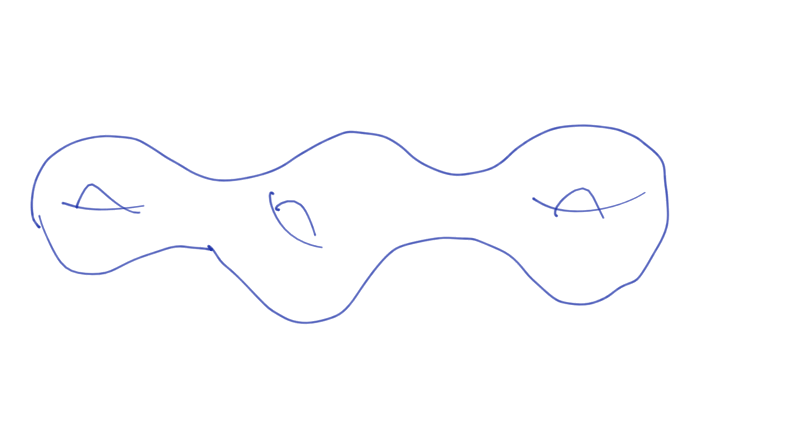
\includegraphics[width=\textwidth]{figures/uniform_lattice.png}
            \caption{Quotient with uniform lattice}
            \label{fig:uniform_lattice}
        \end{subfigure}
        \hfill
        \begin{subfigure}[b]{0.3\textwidth}
            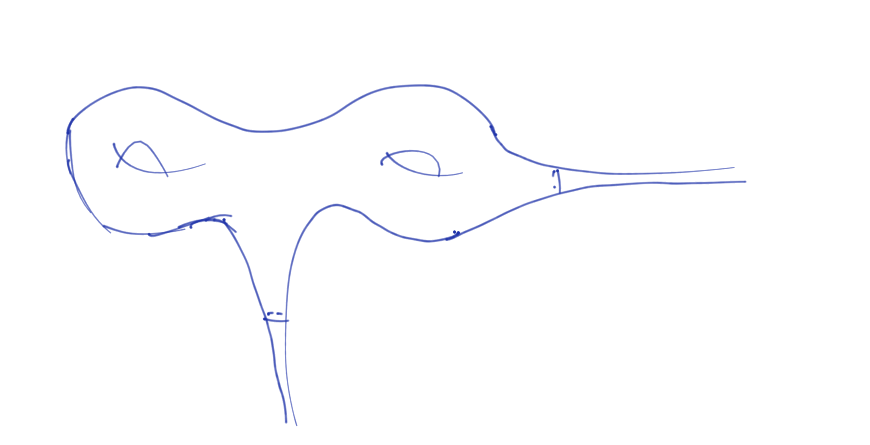
\includegraphics[width=\textwidth]{figures/non_uniform_lattice.png}
            \caption{Quotient with nonuniform lattice}
            \label{fig:nonuniform_lattice}
        \end{subfigure}
        \hfill
        \begin{subfigure}[b]{0.3\textwidth}
            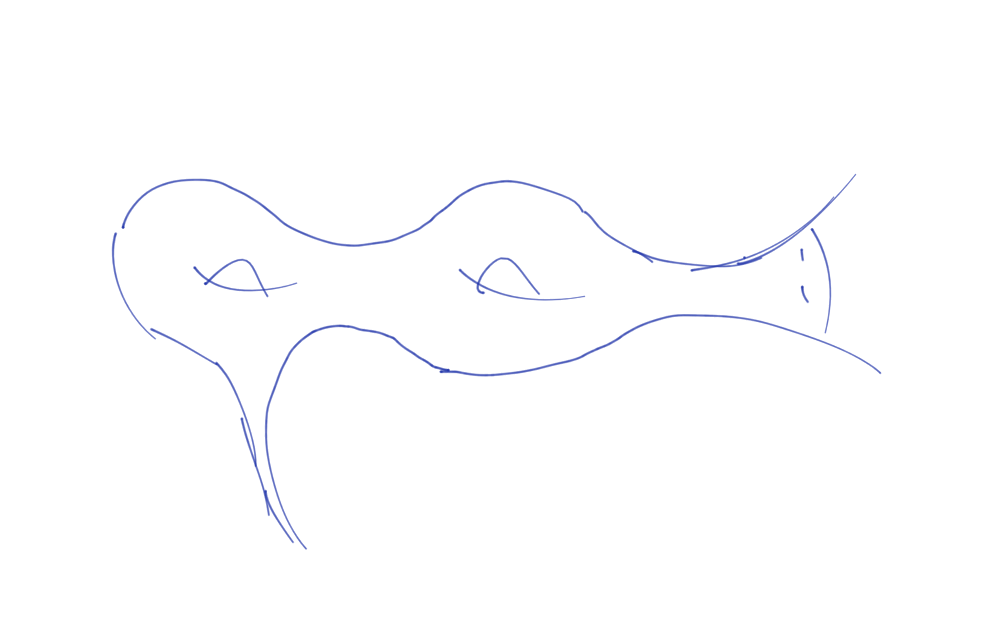
\includegraphics[width=\textwidth]{figures/non_lattice.png}
            \caption{Quotient with nonlattice}
            \label{fig:nonlattice}
        \end{subfigure}
        \caption{Quotients with discrete subgroups of $\SL(2,\mathbb R)$}
        \label{fig:quotients_SL2R}
    \end{figure}
    \item Irreducibility assumption for $\mathbb H^{p,q}$-convex-cocompact and spacelike cocompact representations
    \begin{lemma}
        Let $\rho: \Gamma \to \SO(p,q)$.
        Under certain conditions on $\rho$, exactly one of the three occurs:
        \begin{enumerate}[label=(\roman*)]
            \item $\rho$ is irreducible.
            \item $\rho$ is reducible, with $p \neq q$.\\
            In this case, $\rho(G) \subseteq \mathrm{S}(\OO(p, q') \times \OO(q - q'))$, and the projection of $\rho$ onto $\SO(p,q')$ satisfies some of the certain conditions.
            \item $\rho$ is reducible, with $p = q$.\\
            In this case, $\rho(G)$ preserves two isotropic transverse isotropic subspaces of dimension~$p$.
        \end{enumerate}
    \end{lemma}
    The conditions could include that $\rho$ is $\mathbb H^{p,q}$-convex cocompact or spacelike cocompact.
    \item If $\rho: \Gamma \to \SO(p,q)$ is reducible, $\mathbb H^{p,q}$-convex cocompact, and preserves a \underline{non-degenerate} subspace $V \subseteq \mathbb R^{p,q}$, then $\rho(\Gamma) \subseteq \mathrm{S}(\OO(p,q') \times \OO(q - q'))$.\\
    The idea is to note that since $\rho$ is $\mathbb H^{p,q}$-convex cocompact, it is Anosov, with limit set $\Lambda_\rho$ being negative.
    Since the limit set $\Lambda_\rho$ is contained in $\partial \mathbb H^{p,q}$, we have that $W = \mathrm{span}_\mathbb R (\pi^{-1}(\Lambda_\rho))$ is non-degenerate (since it is generated by negative lines), where $\pi: \mathbb R^{p,q} \to \mathbb H^{p,q}$.
    Thus (by semisimplicity of the representation) there exists a non-degenerate subspace $V \subseteq W$ such that $\rho(\Gamma)$ preserves $V$.
    Letting $q-q'= \dim W$, we have that $\mathrm{sgn}(W) = (0, q-q')$ and $\mathrm{sgn}(V) = (p, q-q')$, implying that $\rho(\Gamma) \subseteq \mathrm{S}(\OO(p,q') \times \OO(q - q'))$.\todo{Not used non-degeneracy of preserved subspace}
    Moreover, when we consider the projection onto V, the limit set does not change and it is negative, and it still satisfies the Anosov property, so it is still $\mathbb H^{p,q'-1}$-convex cocompact.
\end{itemize}
\section{2025-07-10}
\begin{itemize}
    \item The span of the limit set for an Anosov representation is irreducible.
    \begin{lemma}
        Let $\Gamma$ be a non-elementary hyperbolic group and $\rho: \Gamma \to G$ be a $\Theta$-Anosov representation into a linear group $G$.
        Then the span $\mathrm{span}(\Lambda_\rho)$ of the limit set $\Lambda_\rho$ is an invariant subspace of $\rho(\Gamma)$, on which $\rho(\Gamma)$ acts irreducibly.
    \end{lemma}
    \begin{proof}\todo{Do we really need that $\mathrm{vcd}(\Gamma) = p$ and that $\rho$ is $\mathbb H^{p,q}$-convex cocompact?}
        \todo{Maybe we just need (and should somehow use) that $\Lambda_\rho$ is connected?}
        Let $\xi^+(x) \in \Lambda_\rho$ be a point in the limit set, where $x \in \partial_\infty \Gamma$.
        Then by the equivariance of the limit map, we have that $\rho(\gamma) \xi^+(x) = \xi^+(\gamma x) \in \Lambda_\rho$ for all $\gamma \in \Gamma$, so $\Lambda_\rho$ is invariant under the action of $\rho(\Gamma)$.

        To see that $\rho(\Gamma)$ acts irreducibly on $V = \mathrm{span}(\Lambda_\rho)$, we assume the contrary for the sake of contradiction.
        Let $W \subseteq V$ be an invariant subspace of $\rho(\Gamma)$.
        Consider some $\xi^+(\gamma^+) \in \Lambda_\rho$ for $x \in \partial_\infty \Gamma$, and let $\gamma^- \in \Gamma - \{\gamma^+\}$.
        Then there exists a geodesic $\gamma_n$ such that $\lim_{n \to \pm \infty} \gamma_n = \gamma^\pm$.
        If $w \in W - \xi^-(\gamma^-)$, we have that
        \[
        \rho(\gamma_n) w \to \xi^+(\gamma^+) \in W,
        \]
        meaning that $\xi^+(\gamma^+) \in W$.
        This will imply that $\spa(\Lambda_\rho) \subseteq W$, unless every element $w \in W$ is contained in $\xi^-(\gamma^-)$, for all $\gamma^- \in \Gamma - \{\gamma^+\}$.
        In other words, it suffices to exclude the case that 
        \[
        W \subseteq \bigcap_{\gamma^- \in \Gamma - \{\gamma^+\}} \xi^-(\gamma^-) = \left(\xi(\partial_\infty \Gamma-x)\right)^\perp,
        \]
        where the last equality follows from the fact that $\xi^-(y) = \xi^+(y)^\perp$ for all $y \in \partial_\infty \Gamma$.
        
        We claim that the element on the right-hand side is trivial, i.e.\ $W = \{0\}$.
        Indeed, for each two distinct $y, z \in \partial_\infty \Gamma$, we have that $\xi^-(y) \cap \xi^-(z)$ is a subspace of codimension at most one in the hyperplane $\xi^-(y)$.
        This follows from the fact that $\xi^-(y) \neq \xi^-(z)$ for $y \neq z$, since $\xi^+(y) \in \xi^-(y)$ and $\xi^+(y) \cap \xi^-(z) = \{0\}$.
        The same argument applies to the intersection of a finite number of hyperplanes $\xi^-(y_1), \cdots, \xi^-(y_n)$, where $y_i \in \partial_\infty \Gamma$ are distinct.
        Since $\Gamma$ is non-elementary, $\partial_\infty \Gamma$ is infinite and due to finite-dimensionality, we have that the intersection of all hyperplanes $\xi^-(y)$ for $y \in \partial_\infty \Gamma$ is trivial, i.e.\ $W = \{0\}$.
    \end{proof}
    \item A claim for $\mathbb H^{p,q}$-convex cocompact representations of maximal dimension:\todo{Could have something to do with the $j$-crowns in \cite{beyrer2023mathbb}}  
    \begin{claim}
        Let $\rho:\Gamma \to \SO(p,q) \to \mathbb H^{p,q}$ be a $\mathbb H^{p,q}$-convex cocompact representation of maximal dimension.
        Then there exist points $x_1, \cdots, x_{p+1}$ in $\Lambda_\rho$ that span a subspace of signature $(p,1)$, i.e.\ 
        \[
        \spa\{x_1, \cdots, x_{p+1}\} \simeq \mathbb R^{p,1}.
        \]
    \end{claim}
    \item If the above claim is true, then we can deduce the following:
    Reducible $\mathbb H^{p,q}$-convex cocompact representations of maximal dimension restrict to a subrepresentation that is $\mathbb H^{p,q'}$-convex cocompact of maximal dimension.
    \begin{lemma}
        Let $\rho:\Gamma \to \SO(p,q) \to \mathbb H^{p,q}$ be a $\mathbb H^{p,q}$-convex cocompact representation of maximal dimension, where $\Gamma$ is a non-elementary hyperbolic group.
        If $rho$ is reducible, then $\rho(G) \subseteq \mathrm{S}(\OO(p,q') \times \OO(q-q'))$, and the restriction of $\rho$ to the subrepresentation $\rho': \Gamma \to \SO(p,q')$ is $\mathbb H^{p,q'}$-convex cocompact of maximal dimension.
    \end{lemma}
    \begin{proof}
        Let $V = \mathrm{span}(\Lambda_\rho)$ be the span of the limit set $\Lambda_\rho$.
        We know that $V$ is an irreducible subrepresentation of $\rho$, and since $\rho(\Gamma)$ acts cocompactly on $\mathrm{Conv}(\Lambda_\rho)$, we have that $\rho: \Gamma \to \SO(p', q')$ is $\mathbb H^{p',q'}$-convex cocompact, where $(p', q')$ is the signature of $V$.
        
        To show that $p' = p$, let $x_1, \cdots, x_{p+1} \in \Lambda_\rho$ be such that $W = \spa\{x_1, \cdots, x_{p+1}\} \simeq \mathbb R^{p,1}$.
        Then we have that $W \subseteq V$, so $p' \leq p$.
    \end{proof}
\end{itemize}
\section{2025-07-11}
\begin{itemize}
\item There exist no irreducible $\mathbb H^{p,q}$-convex cocompact representations of maximal dimension from $\Sp(2n, \mathbb R)$, except for the $\mathbb H^{p,q}$-convex cocompact subgroups of $\Sp(4, \mathbb R) \simeq \SO(3,2)$ of maximal dimension.
\begin{lemma}
    Let $\rho: \Sp(2n, \mathbb R) \to \SO(p,q)$ be an irreducible representation such that there exists some discrete subgroup $\Gamma \leq G$ for which $\rho_{|\Gamma}$ is an $\mathbb H^{p,q+1}$-convex cocompact representation of maximal dimension.
    Then $n = 2, \mathrm{vcd}(\Gamma) = 2$ and $\rho$ is the special Lie group isomorphism
    \[
    \rho: \Sp(4, \mathbb R) \to \SO(\wedge^2 \mathbb R^4) \simeq \SO(2,3).
    \]
\end{lemma}
\begin{proof}
    Assume that $\rho: \Sp(2n, \mathbb R) \to \SO(p,q)$ is an irreducible representation such that there exists some discrete subgroup $\Gamma \leq G$ for which $\rho_{|\Gamma}$ is an $\mathbb H^{p,q+1}$-convex cocompact representation of maximal dimension.
    Then $\rho$ is $P_1$-Anosov, and $\Gamma$ is $P_\Theta$-Anosov in $\Sp(2n,\mathbb R)$, for
    \[
    \Theta = \{ \alpha \in \Delta(\Sp(2n,\mathbb R)): \langle \alpha, \Lambda \rangle \neq 0 \},
    \]
    where $\Lambda$ is the highest weight of $\rho$.
    In particular, $\Gamma$ is $P_i$-Anosov in $\Sp(2n,\mathbb R)$ for some $1 \leq i \leq n$.
    
    Moreover, since $\Gamma$ is $P_i$-Anosov in $\Sp(2n,\mathbb R)$, we have that the limit set $\partial_\infty \Gamma$ of $\Gamma$ embeds into the flag variety $\mathcal F_\Theta = \Sp(2n,\mathbb R) / P_\Theta$ of $\Sp(2n,\mathbb R)$, which in turn embeds into each flag variety $\mathcal F_j = \Sp(2n,\mathbb R) / P_j$ for each $\alpha_j \in \Theta$.
    Since the Lie algebra of every maximal parabolic subgroup $P_j$ of $\Sp(2n,\mathbb R)$ is given as the intersection of $\sp(2n,\mathbb R)$ with the stepwise upper triangular matrices (where the step is in the $j$-th collumn), we have that the maximal parabolic subgroup with the minimum dimension is $P_1$.
    Equivalently, the flag variety $\mathcal F_1$ has the smallest dimension among all flag varieties $\mathcal F_j$.
    In other words:
    \[
    \dim(\mathcal F_\Theta) \leq \dim(\mathcal F_1) = n-1.
    \]
    Using the equality of Bestvina-Mess, we have that $\mathrm{vcd}(\Gamma) = \dim(\partial_\infty \Gamma) + 1 \leq \dim(\mathcal F_\Theta) + 1 \leq n$.
    Combining with the fact that the positive weights of $\rho$ are at most $\min\{p,q\}$, we have that
    \[
    \mathcal P_{>0}(\rho) \leq p = \mathrm{vcd}(\Gamma) \leq n \leq \dim(\mathcal F_1) + 1.
    \]

    Since $\rho$ is an irreducible representation of $\Sp(2n, \mathbb R)$, we know that it is a subrepresentation of the tensor product of symmetric powers of exterior powers of the standard representation $\mathbb R^{2n}$:
    \[
    \rho: \Sp(2n, \mathbb R) \to \bigotimes_{i=1}^n \Sym^{k_i}(\wedge^i \mathbb R^{2n}),
    \]
    where $k_i \geq 0$ are integers.
    If a symmetric power of the exterior power $\wedge^i \mathbb R^{2n}$ appears in the product, then the highest weight of $\rho$ is given by $\Lambda = L_1 \oplus +\cdots + L_i$, which has an orbit of cardinality $2^i \cdot n!/i!$ through the Weyl group.
    Since each such representation is self-dual, half of these weights are positive, meaning that the number of positive weights is at least $2^{i-1} \cdot n (n-1) \cdots (n-i+1)$.
    
    Clearly, for $n \geq 3$, these are more than $n$ positive weights, so we must have $n = 2$ and thus $i = 1,2$.
    If $i = 1$, then the standard representation appears in the product.
    Since it is symplectic it needs to appear either along with another exterior power that carries a symplectic structure, or to appear as a symmetric power of the standard representation.
    Since the only exterior powers that appear as factors are $\mathbb R^{2n}$ and $\wedge^2 \mathbb R^{2n}$, the first option is not feasible.
    On the other hand, neither is the second option, since any symmetric power of the standard representation will have more than $n$ positive weights.

    Hence we must have $i = 2$, with highest weight $\Lambda(\Sym^k(\wedge^2 \mathbb R^{2n})) = 2k(L_1 + L_2)$.
    The orbit of the highest weight has at least two weights: $2k(L_1 \pm L_2)$.
    If $k > 1$, then there exist also positive weights that are not in the orbit of the highest weight, so we must have $k = 1$.
    Said differently, the only possibility is the special Lie group isomorphism of $\Sp(4, \mathbb R)$ in the orthogonal complement $(\mathbb R \omega)^\perp \subseteq \wedge^2 \mathbb R^4$, where $\omega$ is the symplectic form on $\mathbb R^4$ preserved by $\Sp(4, \mathbb R)$.
    \[
    \wedge^2\left(\mathrm{std}\right): \Sp(4, \mathbb R) \to \SO(2,3).
    \]
\end{proof}
\end{itemize}
\section{2025-07-15}
\begin{itemize}
\item Most irreducible representation from $\SO(n+1,n)$ to some $\SO(p,q)$ that restricts to a convex-cocompact representation of maximal dimension are the standard representation.
\begin{lemma}
    Let $\rho: \SO(n+1,n) \to \SO(p,q)$ be an irreducible representation such that there exists some discrete subgroup $\Gamma \leq G$ for which $\rho_{|\Gamma}$ is an $\mathbb H^{p,q+1}$-convex cocompact representation of maximal dimension.
    Then $\rho$ is either the standard representation $\SO(n+1,n) \to \SO(n+1,n)$, or it is the adjoint representation of $\SO(2,1)$ or $\SO(3,2)$:
    \begin{align*}
        \Ad: \Gamma \leq \SO(2,1) \to \SO(1,2), \text{ with } \mathrm{vcd}(\Gamma) = 1\\
        \Ad: \Gamma \leq \SO(3,2) \to \SO(4,6), \text{ with } \mathrm{vcd}(\Gamma) = 4.
    \end{align*}
\end{lemma}
\begin{proof}
    Assume that $\rho: \SO(n+1,n) \to \SO(p,q)$ is an irreducible representation such that there exists some discrete subgroup $\Gamma \leq G$ for which $\rho_{|\Gamma}$ is an $\mathbb H^{p,q+1}$-convex cocompact representation of maximal dimension.
    Then $\rho$ is $P_1$-Anosov, and $\Gamma$ is $P_\Theta$-Anosov in $\SO(n+1,n)$, for some $\Theta \subseteq \{1,\ldots,n\}$.
    In particular, $\partial_\infty \Gamma$ embeds into the flag variety $\mathcal F_\Theta = \SO(n+1,n) / P_\Theta$ of $\SO(n+1,n)$, which in turn embeds into each flag variety $\mathcal F_j = \SO(n+1,n) / P_j$ for each $\alpha_j \in \Theta$.
    Since the maximal parabolic subgroups of $\SO(n+1,n)$ are the stabilizers of isotropic $k$-subspaces for $k = 1, \ldots, n$, whose matrix form is given by the stepwise upper triangular matrices, we have that the maximal parabolic subgroup with the minimum dimension is $P_1$, or equivalently, the flag variety $\mathcal F_1$ has the smallest dimension among all flag varieties $\mathcal F_j$.
    Using the result of Bestvina-Mess, we have that 
    \[
    \mathrm{vcd}(\Gamma) = \dim(\partial_\infty \Gamma) + 1 \leq \dim(\mathcal F_{\{\mathbf a_1\}}) + 1 \leq 2n+1.
    \]
    Combining with the fact that the positive weights of $\rho$ are at most $\min\{p,q\}$, we have that
    \[
    \sharp \mathcal P_{>0}(\rho) \leq p = \mathrm{vcd}(\Gamma) \leq 2n+1.
    \]

    Since $\rho$ is an irreducible representation of $\SO(n+1,n)$, we know that it is a subrepresentation of the tensor product of symmetric powers of exterior powers of the standard representation $\mathbb R^{n+1,n}$:
    \[
    \rho: \SO(n+1,n) \to \bigotimes_{i=1}^n \Sym^{k_i}(\wedge^i \mathbb R^{n+1,n}),
    \]
    where $k_i \geq 0$ are integers.

    It will be useful to note that the weights of each exterior (or symmetric) power are also weights of every higher exterior (or symmetric) power, since $0$ is a weight of the standard representation.
    This implies that exterior powers higher than $3$ do not appear in the product, since $\wedge^3 \mathbb R^{n+1,n}$ has at least
    \[
    \binom{n}{3} + 2 \cdot \binom{n}{2} + n 
    \]
    positive weights (as sums $L_i + L_j + L_k, L_i + L_j, L_i - L_j, L_i$ for $1 \leq i < j < k \leq n$), which is larger than $2n+1$ for $n \geq 3$.

    On the other hand, we note that the exterior square $\wedge^2 \mathbb R^{n+1,n}$ is the adjoint representation which can be found to land in $\SO(n^2, n(2n+1))$, which means that it can't appear in the product for $n \geq 3$.

    Symmetric powers of the standard representation $\Sym^k(\mathbb R^{n+1,n})$ can not appear either for $k \geq 2$, since its weights are given by $\pm 2L_i, \pm L_i, \pm L_i \pm L_j$ for $1 \leq i < j \leq n$, so the number of positive ones exceeds $2n+1$.
    Similarly we exclude the case of products involving $\mathbb R^{n+1,n}$ and $\wedge^2 \mathbb R^{n+1,n}$.
\end{proof}
\end{itemize}
\section{2025-09-04}
\begin{itemize}
    \item Let $\Gamma$ be a non-elementary hyperbolic group and $\rho: \Gamma \to G$ be a $\Theta$-Anosov representation into a $\SL(d,\mathbb R)$.
    Then for $\alpha_k \in \Theta$, there exists no subspace in $\mathcal G_k(R^d)$ that is in all the subspaces $\xi^{d-k}(x)$ for $x \in \partial_\infty \Gamma$.
    \begin{proof}
        What we want to show is that
        \[
        \cap_{x \in \partial_\infty \Gamma} \xi^{d-k}(x) = \{0\}.
        \]
        Let $x \neq y \in \partial_\infty \Gamma$.
        Then $\xi^{d-k}(x) \cap \xi^{d-k}(y)$ is a subspace of codimension at least one in $\xi^{d-k}(x)$, since $\xi^{d-k}(x) \neq \xi^{d-k}(y)$.
        The same arguement implies that in each intersection, the dimension decreases by at least one.
        Since $\Gamma$ is non-elementary, $\partial_\infty \Gamma$ is infinite, so the intersection must be trivial.
    \end{proof}
    \item Let $\Gamma$ be a non-elementary hyperbolic group and $\rho: \Gamma \to \SL(d,\mathbb R)$ be an $\mathbb H^{p,q}$-convex cocompact representation.
    If $\Omega \subseteq \mathbb R^{p,q}$ is a properly convex domain preserved by $\rho(\Gamma)$, then the limit set $\Lambda_\rho$ is contained in the closure $\overline{\mathbb P(\Omega)}$ of the projectivization $\mathbb P(\Omega)$ of $\Omega$.
    \begin{proof}
        Since the action of $\Gamma$ on $\xi^1(\partial_\infty \Gamma)$ is minimal, i.e.\ every orbit is dense, it suffices to show that there exists some $x \in \partial_\infty \Gamma$ such that $\xi^1(x) \in \overline{\mathbb P(\Omega)}$.
    \end{proof}
    \item Let $\rho: \Gamma \to \SO(p, q+1)$ be an $\mathbb H^{p,q}$-convex cocompact representation, and $\Omega \subseteq \mathbb R^{p,q+1}$ be a properly convex domain preserved by $\rho(\Gamma)$.
    Then the lift of the limit set $\pi^{-1}(\Lambda_\rho)$ under the double covering $\pi: \mathbb S^{p-1} \times \mathbb S^q \to \partial \mathbb H^{p,q}$ has two connected components, each of which is a copy of $pi^{-1}(\Lambda_\rho)$, in the sense that when restricted to each, $\pi$ is a homeomorphism onto $\Lambda_\rho$.
    \begin{proof}
        First we show that $\pi^{-1}(\Lambda_\rho)$ is not connected, i.e.\ it has at least two connected components.
        Assume the contrary for the sake of contradiction.
        Then for $x \in \pi^{-1}(\Lambda_\rho)$, we have that $-x \in \pi^{-1}(\Lambda_\rho)$ as well.
        Since $\Omega$ is properly convex, there exists a hyperplane $H$ that does not intersect $\bar \Omega$.
        Let $\gamma: I \to \pi^{-1}(\Lambda_\rho)$ be a path from $x$ to $-x$.
        Then $\gamma$ must intersect $H$ at some point $\gamma(t_0)$, which is a contradiction since $\pi(\gamma(t_0)) \in \Lambda_\rho \subseteq \overline{\mathbb P(\Omega)}$.
        In particular, we have shown that each component of $\pi^{-1}(\Lambda_\rho)$ contains at most one lift of each point in $\Lambda_\rho$.

        To show that it has at most two components, it suffices to show that the restriction of $\pi$ to each component is surjective, since $\pi$ is a double covering.
        Let $\tilde x \in \pi^{-1}(\Lambda_\rho)$ be a point in some component, that projects to $\pi(\tilde x) = x \in \Lambda_\rho$.
        Then for any $y \in \Lambda_\rho$, there exists a path $\gamma$ in $\Lambda_\rho$ from $x$ to $y$.
        Then it lifts to a path $\tilde \gamma$ in $\pi^{-1}(\Lambda_\rho)$ from $\tilde x$ to some lift of $y$, which will be contained in the same component as $\tilde x$.
        Thus the restriction of $\pi$ to the component is surjective.
    \end{proof}
\end{itemize}
\section{2025-09-08 -- meeting -- Limit set regularity rigidity}
\subsection{Why deformations are interesting}
Short answer: they give us representations of discrete groups that do not come from a representation of a Lie group.

Let $G$ be a real semisimple Lie group.
In general, we are interested in lattices of $G$, because roughly they give us manifolds or orbifolds.
However, lattices are rigid in higher rank Lie groups, in the sense that there only a few of them.
This is because under the conditions of the Margulis rigidity theorem, any representation of a lattice $\Gamma \leq G$ into another Lie group $H$ can be extended to a representation of $G$ into $H$.
However, there exist finitely many representations of $G$ into $H$, which can be studied individually.

For this reason, we are led to consider discrete subgroups of $G$ that admit deformations (whose image is not a discrete group and) which do not extend to $G$.
If we take for instance $Z \leq G$ a rank-1 Lie subgroup of $G$, then we can take $\Gamma \leq Z$ a lattice, and $\rho: Z \to G$ a representation for which $\rho_{|\Gamma}$ is Anosov.
Then it is known that the deformations of $\rho_{|\Gamma}$ are Anosov as well.
In this way, we obtain an infinite family of interesting representations $\rho_t$ which do not extend to $G$.
\subsection{Rigidity with respect to regularity}
Let $\Gamma \leq G$ be a discrete subgroup of the semisimple Lie group $G$ and $\rho: \Gamma \to H$ be a representation into another semisimple Lie group $H$, that is assumed to be Anosov.
One would like to know when this representation is "banal", in the sense that it comes from a representation of $G$ into $H$.
One way to do this is to look at the regularity of the limit set $\Lambda_\rho$.

In the "banal" case, the limit set $\Lambda_\rho$ is very regular.

\subsubsection{$\mathrm{AdS}$-quasifuchsian representations}
In the case of $\mathrm{AdS}$-quasifuchsian representations, one has the result of \cite{glorieux2018regularity}.
We recall:
\begin{definition}
    Let $\Gamma \leq \SO(n,2)$ be a discrete subgroup.
    Then:
    \begin{enumerate}
        \item $\Gamma$ is $\mathrm{AdS}^{n+1}$-quasifuchsian if it is $\mathbb H^{n,1}$-convex cocompact of maximal dimension, i.e.\ it acts properly discontinuously and cocompactly on some properly convex closed subset of $\mathbb H^{n,1}$ and its limit set $\Lambda_\Gamma \subseteq \partial \mathbb H^{n,1}$ is homeomorphic to $\mathbb S^{n-1}$.
        \item $\Gamma$ is $\mathrm{AdS}^{n+1}$-Fuchsian if it is $\mathrm{AdS}^{n+1}$-quasifuchsian and preserves a totally geodesic copy of $\mathbb H^n \subseteq \mathbb H^{n,1}$.
    \end{enumerate}
\end{definition}

One knows that the limit set of an $\mathrm{AdS}^{n+1}$-Fuchsian representation is (smooth and hence) $\mathcal C^1$.
The reason for that is that one can show that it will act cocompactly on the totally geodesic copy of $\mathbb H^n$ that it preserves, so the boundary will be a regular sphere of dimension $n-1$.
The result of \cite{glorieux2018regularity} states that $\mathcal C^1$-regularity of the limit set is rigid, in the sense that it characterizes the $\mathrm{AdS}^{n+1}$-Fuchsian representations among quasifuchsian ones:
\begin{theorem}[Theorem 1.3 of \cite{glorieux2018regularity}]
Let $\Gamma$ be an $\mathrm{AdS}^{n+1}$-quasifuchsian group.
Then its limit set $\Lambda_\Gamma$ is a $\mathcal C^1$ submanifold of $\partial \mathrm{AdS}^{n+1}$ if and only if $\Gamma$ is $\mathrm{AdS}^{n+1}$-Fuchsian.
\end{theorem}
Hence in a sense, regularity of the limit set is only possible for examples that come from the rank-1 case (i.e.\ $\SO(n,1)$).

\subsubsection{Convex-cocompact representations}
Here similarly we have that $\mathcal C^1$-regularity characterises strict convexity:
\begin{theorem}[Benoist - Convex divisibles I]
    Let $\Omega$ be a divisible convex subset of $\mathbb P(\mathbb R^d)$ divided by $\Gamma$.
    Then the following are equivalent:
    \begin{enumerate}
        \item The metric space $(\Omega, d_\Omega)$ is Gromov-hyperbolic.
        \item The convex set $\Omega$ is strictly convex.
        \item The boundary $\partial \Omega$ is $\mathcal C^1$.
        \item The group $\Gamma$ is Gromov-hyperbolic.
    \end{enumerate}
\end{theorem}
On the other hand we have that $\mathcal C^2$-regularity is even more rigid, since it characterises ellipsoids among strictly convex sets:
\begin{theorem}[Benoist ?]
    Let $\Omega$ be a strictly convex divisible convex subset of $\mathbb P(\mathbb R^d)$ divided by $\Gamma$.
    Then $\partial \Omega$ is $\mathcal C^2$ if and only if $\Omega$ is an ellipsoid.
\end{theorem}
\subsubsection{A few conjectures}
In the spirit of the above, we can make the following conjectures:
\begin{conjecture}\label{conj:limit_set_regularity_rigidity}
    Let $\Gamma \leq \SO(p,q)$ be $\mathbb H^{p,q}$-convex cocompact of maximal dimension.
    Then its limit set $\Lambda_\Gamma$ is a $\mathcal C^2$ submanifold of $\partial \mathbb H^{p,q}$ if and only if $\Gamma$ is a lattice of a Lie subgroup $G$ of rank $1$ of $\SO(p,q)$.

    Moreover, the groups $G$ that appear can be classified into some families of representations.
\end{conjecture}
\begin{conjecture}
    If $q \leq p$ or $p \geq 3$, then \cref{conj:limit_set_regularity_rigidity} holds for $\mathcal C^1$-regularity.
\end{conjecture}
Note however that $\mathcal C^1$-regularity is not always attained.
For instance, if $\rho: \pi_1(S) \to \SO(2,3)$ is a Hitchin representation, then its limit set is a $\mathcal C^1$-submanifold and not $\mathcal C^2$ unless it is Hitchin Fuchsian (?).

\section{2025-09-15 -- comité de suivi -- geodesic flow and Anosov representations}
This was a crash course by Nicolas and Daniel.\\
Unless otherwise stated, $M$ will be a compact manifold with strictly negative curvature.

\subsection{Geodesic flow basics}
Then we can define the geodesic flow $\phi_t: T^1 M \to T^1 M$ on the unit tangent bundle $T^1 M$ of $M$.

Note that the unit tangent bundle of the universal cover $\widetilde M$ of $M$ can be identified by a pair of points in the boundary at infinity $\partial_\infty \widetilde M$ and a real number:
\[
T^1 \widetilde M \simeq \partial_\infty \widetilde M \times \mathbb R.
\]
The boundaries at infinity designate a geodesic in $\widetilde M$, and the real number designates a point on that geodesic.

\begin{definition}
    A closed orbit of the geodesic flow $\phi_t$ is a set of the form
    \[\{\phi_t(v): t \in \mathbb R\},
    \]
    where $v \in T^1 M$ is such that $\phi_T(v) = v$ for some $T > 0$.
\end{definition}
Clearly, closed geodesics in $M$ correspond to closed orbits of the geodesic flow, which in turn correspond to conjugacy classes of primitive elements in $\pi_1(M)$, which are known to be in bijection with free homotopy classes of closed curves in $M$.
In particular, a reparametrization does not influence the closed orbits of the flow (it only changes their period).

\begin{definition}
    Let $f: M \to \mathbb R_{>0}$ be a positive function.
    Then there exists a flow $\phi^f_t: T^1 M \to T^1 M$ such that the generator of $\phi^f_t$ is $f$ times the generator of $\phi_t$, i.e.\ 
    \[
    \left. \frac{d}{dt} \right|_{t=0} \phi^f_t(v) = f (v) \cdot \left. \frac{d}{dt} \right|_{t=0} \phi_t(v).
    \]
    We call $\phi^f_t$ the reparametrization of $\phi_t$ by $f$.
\end{definition}
Note that if $T > 0$ is the period of a closed orbit starting at $v \in T^1 M$, then the period $T'$ of the closed orbit starting at $v$ for the reparametrized flow $\phi^f_t$ is given by
\[
T' = \int_0^T f(\phi_t(v)) dt.
\]\todo{Why?}
Moreover, if $\mu$ is a $\phi_t$-invariant probability measure on $T^1 M$, then $\mu^f = f \d \mu$ is a $\phi^f_t$-invariant probability measure on $T^1 M$.

\begin{definition}[Exponential mixing]
    Let $\psi_t$ be a flow on a metric space $X$ and $\mu$ an invariant measure.
    Then we say that $\psi_t$ mixes exponentially with respect to $\mu$ if for all $\alpha$-Hölder functions $f,g: X \to \mathbb R$:
    \[
    \int_X f(\psi_t(x)) g(x) d\mu(x) \to \int_X f d\mu \int_X g d\mu
    \]
\end{definition}
The classical tools to show exponential mixing are based on the regularity of the stable and unstable leaves of the flow.

\begin{definition}
    Let $\psi_t$ be a flow on a metric space $X$.
    The strongly and weakly stable leaves of $\psi_t$ at $x \in X$ are given by
    \begin{align*}
        W^{ss}(x) &= \{y \in X: d(\psi_t(x), \psi_t(y)) \to 0 \text{ as } t \to +\infty\}\\
        W^{ws}(x) &= \{y \in X: d(\psi_t(x), \psi_t(y)) \text{ is bounded for } t > 0\}.
    \end{align*}
    Similarly, the strongly and weakly unstable leaves of $\psi_t$ at $x \in X$ are given by
    \begin{align*}
        W^{su}(x) &= \{y \in X: d(\psi_t(x), \psi_t(y)) \to 0 \text{ as } t \to -\infty\}\\
        W^{wu}(x) &= \{y \in X: d(\psi_t(x), \psi_t(y)) \text{ is bounded for } t < 0\}.
    \end{align*}
\end{definition}
Under certain conditions, these define folitations of a certain regularity.
For instance, in the geodesic flow of the hyperbolic space, the strongly stable leaves are the horocycles based at the forward endpoint of the geodesic in the boundary at infinity.
The weakly stable leaves are the sets of geodesics that share the same forward endpoint.

Given an endpoint $p \in \partial_\infty \mathbb H^n$ we can define the Busemann function based at $p$, which measures the distances of points as seen from the point $p$ at infinity.
In particular, for $x,y \in T^1 \mathbb H^n$ pointing towards $p$ (in which case we have $y \in W^{ws}(x)$), we define
\[
B_p(x,y) = \lim_{t \to \infty} d(\phi_t(x), \phi_t(y)).
\]

\subsection{Geodesic flow and Anosov representations -- Sambarino's flow}
Let $\rho: \pi_1(M) \to G$ be a $\Theta$-Anosov representation into a semisimple Lie group $G$.
The for every functional $\alpha \in \mathfrak a^*$ that is positive on the Weyl chamber $\mathfrak a^+$ and that is of the form
\[
\alpha = \sum_{\theta \in \Theta} \alpha_\theta \omega_\theta,
\]
where $\omega_\theta$ are the fundamental weights of $G$, we can construct a reparametrization (depending on the choice of $\alpha$ and the representation) $\phi^f$ of the geodesic flow $\phi_t$ on $T^1 M$ such that 
\[
\mathcal L_f(\gamma) = \alpha(\lambda(\rho(\gamma))),
\]
where $\mathcal L_f(\gamma)$ is the length of the geodesic corresponding to $\gamma \in \pi_1(M)$ for the reparametrized flow $\phi^f_t$.
Note that although the reparametrized flow is not necessarily a geodesic flow for some metric, it still has the same closed orbits as the original geodesic flow, which are in bijection with conjugacy classes of primitive elements in $\pi_1(M)$.
Using this we can obtain estimates for the number of closed orbits of the flow $\phi^f_t$ of a certain bounded length:
\[
\sharp\{[\gamma] \in [\pi_1(M)]: \mathcal L_f(\gamma) \leq R\} \sim \frac{e^{\delta_1(\rho)R}}{\delta_1(\rho) R},
\]

In the case of projective Anosov representations into $\SL(d,\mathbb R)$, we have (probably due to Daniel) that there exists some $\epsilon > 0$ such that 
\[
\sharp\{[\gamma] \in [\pi_1(M)]: \alpha(\lambda(\rho(\gamma))) \leq R\} \sim \frac{e^{\delta_1(\rho)R}}{\delta_1(\rho) R} \cdot (1 + O(e^{-\epsilon R})).
\]
For this, we need the fact that the reparametrized flow $\phi^f_t$ mixes exponentially with respect to the Borel-Margulis measure.
Since its leaves are only Hölder, the classical tools do not apply.
For this, we embed it into a larger smooth flow for which the classical tools apply, and then we restrict back to our flow.
\begin{theorem}[DMS]
    Let $\rho: \pi_1(M) \to \SL(d,\mathbb R)$ be a projective Anosov representation.
    Then there exists a reparametrization $\phi^\rho_t$ of the geodesic flow $\phi_t$ on $T^1 M$ for which $\mathcal L_{\phi^\rho}(\gamma) = \lambda_1(\rho(\gamma))$ for all $\gamma \in \pi_1(M)$.

    There also exists a smooth flow $\psi_t$ on a smooth manifold $N$, smooth foliations $\mathcal W^{ss}_\psi, \mathcal W^{su}_\psi$ of $N$ and a Hölder embedding $F: T^1 M \to N$ that conjugates $\phi^\rho_t$ with the restriction of $\psi_t$ to $F(T^1 M)$, such that $F(\mathcal W^{ss}_{\phi^\rho}) = \mathcal W^{ss}_\psi \cap F(T^1 M)$ and $F(\mathcal W^{su}_{\phi^\rho}) = \mathcal W^{su}_\psi \cap F(T^1 M)$. 
\end{theorem}
Note that the flow $\phi^\rho_t$ is different than the one constructed by Sambarino.

\begin{example}
    Let $M$ be a compact hyperbolic surface and $\rho: \pi_1(M) \to \SO(3,1) \leq \SL(4,\mathbb R)$ be a quasi-Fuchsian representation.
    Then $N = T^1 \mathbb H^3 / \rho(\pi_1(M)) \simeq T^1(M \times \mathbb R)$.
\end{example}
\subsection{Ehresmann - Thurston principle}
For a $(G, G/H)$-structure on $M$ we can define the holonomy representation $\rho: \pi_1(M) \to G$ and the developing map $\mathrm{dev}: \widetilde M \to G/H$.
Then we have the following:
\begin{theorem}[Ehresmann - Thurston principle]
    If $\rho'$ is sufficiently close to $\rho$, then there exists a $(G, G/H)$-structure on $M$ with holonomy $\rho'$.
\end{theorem}
\section{2025-09-16}
\begin{proposition}
The adjoint representation of $\GL(n, \mathbb R)$ lies into $\SL(\gl(n, \mathbb R))$.    
\end{proposition}
\begin{proof}
Recall that for a vector space $V$ we have the identification
\begin{align*}
    V &\otimes V^* \simeq \mathrm{End}(V)\\
    v \otimes \varphi &\mapsto (w \mapsto \varphi(w) v)\\
    E_{ij} &\mapsfrom e_i \otimes e^j.
\end{align*}
Then we can see left and right multiplication by $g$ (acting on $\mathfrak{gl}(n, V)$) as endomorphisms of $V \otimes V^*$:
\begin{align*}
    L_g = g \otimes \mathrm{id}_{V^*}\\
    R_g = \mathrm{id}_V \otimes g^t.
\end{align*}
Then the adjoint representation is given by $\Ad(g) = L_g \circ R_{g^{-1}} = g \otimes (g^{-1})^t$.
Knowing that $\mathrm{det}(A \otimes B) = (\mathrm{det} A)^{\dim B} (\mathrm{det} B)^{\dim A}$, we have that $\mathrm{det}(\Ad(g)) = 1$ for all $g \in \GL(n, \mathbb R)$.    
\end{proof}
\section{2025-09-21}
\begin{itemize}
    \item
The limit set of a uniform lattice of $\SO(n,1)$ is the full boundary $\partial \mathbb H^n \simeq \mathbb S^{n-1}$.
Recall that the limit set is given as $\Lambda_\Gamma = \overline{\Gamma \cdot x} \cap \partial \mathbb H^n$ for some $x \in \mathbb H^n$, and $\partial \mathbb H^n$ is the Gromov boundary of $\mathbb H^n$.
\begin{proposition}
    Let $\Gamma \leq \SO(n,1)$ be a uniform lattice.
    Then its limit set is the full boundary $\partial \mathbb H^n$.
\end{proposition}
\begin{proof}
    Since the action is cocompact, there exists a compact set $K \subseteq \mathbb H^n$ such that $\Gamma \cdot K = \mathbb H^n$.
    Without loss of generality, we can assume that $o \in K$.
    Let $\xi \in \partial \mathbb H^n$, and let $r: \mathbb N \to \mathbb H^n$ be a geodesic ray such that $r(\infty) = \xi$.
    Then for every $n$, there exists $\gamma_n \in \Gamma$ such that $\gamma_n^{-1} r_n \in K$.
    In particular, $d(\gamma_n^{-1} r_n, o) = d(r_n, \gamma_n o) \leq \mathrm{diam}(K)$ is bounded.
    By the Fellow Traveller property, this implies that $\gamma_n o \to \xi$ as $n \to \infty$.
\end{proof}
\end{itemize}
\section{2025-09-23}
\begin{itemize}
    \item Labourie's lemma is correct in dimension $1$ and when the group $G$ is very large.
    \begin{proposition}
        Let $G$ be a subgroup of $\SL(d,\mathbb R)$, such that
        \[
        \dim G \geq d-1.
        \]
        Then for every $l \in \mathbb P(\mathbb R^d), W \in \mathcal G_{d-k}(\mathbb R^d)$, there exists $g \in G$ such that $g l \oplus W = \mathbb R^d$.
    \end{proposition}
    \begin{proof}
        We know the orbit of a Lie group is an immersed submanifold of $\mathbb R^d$.
        In our case, $G \cdot l$ is an immersed submanifold of $\mathbb P(\mathbb R^d)$ of dimension at least $d-1$.
        Since the inclusion map is an immersion, its differential is injective. But since the dimension of the domain and codomain are equal, it is an isomorphism, meaning that it is a diffeomorphism onto its image.
        
        Thus $G \cdot l$ contains an open neighborhood of $l$ in $\mathbb P(\mathbb R^d)$ and no projective hyperplane can contain an open set, so there exists $g \in G$ such that $g l \oplus W = \mathbb R^d$.
    \end{proof}
    \item Transversality in Grassmanian coordinates:
    \begin{proposition}
        Let $P \in \mathcal G_k(\mathbb R^d)$ and $Q \in \mathcal G_{d-k}(\mathbb R^d)$ be two complementary subspaces.
        We define $U_Q$ and $U_P$ as the transverse subspaces to $Q$ and $P$ respectively:
        \begin{align*}
            U_Q &= \{W \in \mathcal G_k(\mathbb R^d): W \oplus Q = \mathbb R^d\}\\
            U_P &= \{W \in \mathcal G_{d-k}(\mathbb R^d): W \oplus P = \mathbb R^d\}.
        \end{align*}
        Then we have the following parametrizations of the Grassmanians:
        \begin{align*}
            \mathcal L(Q, P) &\to U_Q \subseteq \mathcal G_k(\mathbb R^d)\\
            X &\mapsto \mathrm{graph}(X)\\
            \mathcal L(P, Q) &\to U_P \subseteq \mathcal G_{d-k}(\mathbb R^d)\\
            Y &\mapsto \mathrm{graph}(Y),
        \end{align*}
        where $\mathcal L(A,B)$ is the space of linear maps from $A$ to $B$.

        In these coordinates, the transversality condition of a flag $(\mathrm{graph}(X), \mathrm{graph}(Y)) \in U_Q \times U_P \subseteq \mathcal G_k(\mathbb R^d) \times \mathcal G_{d-k}(\mathbb R^d)$ is:
        \[
        \mathrm{graph}(X) \pitchfork \mathrm{graph}(Y) \iff \mathrm{Id} - YX \in \GL(Q).
        \]

        Fix a basis of $\mathbb R^d$ adapted to the decomposition $\mathbb R^d = P \oplus Q$.
        In these coordinates for $\GL(d,\mathbb R)$ we have that the transversality condition under the action of $g \in \GL(d, \mathbb R)$ is given by
        \[
        g \cdot \mathrm{graph} (X) \pitchfork \mathrm{graph}(Y) \iff (CX + D) - Y(AX + B) \in \GL(Q),
        \]
        where
        \[g = \begin{pmatrix}
            A & B\\
            C & D
        \end{pmatrix}\]
        in the chosen basis, i.e.\ $A: P \to P, B: Q \to P, C: P \to Q, D: Q \to Q$, given by $\mathrm{pr}_P g_{|P}, \mathrm{pr}_P g_{|Q}, \mathrm{pr}_Q g_{|P}, \mathrm{pr}_Q g_{|Q}$ respectively.
    \end{proposition}
    This allows us either to disprove Labourie's property by finding $X,Y$ such that for all $A, B, C, D$ the above is not invertible, or to prove it for flags in $U_Q \times U_P$ by finding $A, B, C, D$ for all $X,Y$ such that the above is invertible.
    \item It feels like all irreducible representations of $\SL(2,\mathbb R)$ satisfy Labourie's property for $k = 1$.
    We have that
    \[
    \mathrm{span}\left(\rho(\SL(2,\mathbb R)) e_1^i\right) = \mathbb R^d
    \]
\end{itemize}
\section{2025-09-28}
\begin{enumerate}
    \item Let $\mathfrak g$ be a simple Lie algebra, whose Cartan involution is $\theta$.
    If $\sigma$ is another involution of $\mathfrak g$ that commutes with $\theta$.
    Then the restriction of the adjoint representation $\ad_{\mathfrak g^\sigma}$ on the fixed point set preserves the antifixed point set $\mathfrak g^{-\sigma}$.
    This is not always irreducible:
    \begin{example}
        Let $\mathfrak g = \mathfrak{sl}(n, \mathbb R)$, $\sigma(X) = I_{p,q} X I_{p,q}$.
        Then
        \[
        \mathfrak g^\sigma = \left\{\begin{pmatrix}
            A & 0\\
            0 & D
        \end{pmatrix}: A \in \mathfrak{sl}(p, \mathbb R), D \in \mathfrak{sl}(q, \mathbb R)\right\},
        \mathfrak g^{-\sigma} = \left\{\begin{pmatrix}
            0 & B\\
            C & 0
        \end{pmatrix}: B \in M_{p,q}(\mathbb R), C \in M_{q,p}(\mathbb R)\right\}.
        \]
        Clearly $\ad_{\mathfrak g^\sigma}$ is not irreducible on $\mathfrak g^{-\sigma}$, and admits two invariant subspaces.
        \item Regarding the above situation, it is possibly correct that if the representation is not irreducible, then it admits two invariant subspaces, each of which is isotropic for the Killing form and which are permuted by the Cartan involution.
    \end{example}
\end{enumerate}
\section{2025-09-29}
\begin{enumerate}
    \item Limit sets of uniform lattice and convex-cocompact subgroups.
    
    Let $G$ be a rank $1$ semisimple Lie group, and $\phi: G \to H$ be a Lie group morphism, where $H$ is a semisimple Lie group.
    Then there exists a parabolic subgroup $P_H$ of $H$ such that $\phi_{\mid \Gamma}$ is $P_H$-Anosov for every uniform lattice $\Gamma$ of $G$.
    In fact, for every uniform lattice $\Gamma$ of $G$, the limit set is the same, and it is a smooth embedded submanifold of $G/P_H$.

    In fact, denoting with $P_G$ the unique parabolic proper subgroup of $G$, there exists an equivariant smooth embedding $\xi_G: G/P_G \to H/P_H$, and the limit set of $\phi_{\mid \Gamma}$ is $\xi_G(G/P_G)$.

    If $\Gamma$ is convex-cocompact, then it has a limit set $\Lambda_\Gamma \subseteq \partial_\infty (G/K) = G/P_G$ that can be identified with the Gromov boundary of $\Gamma$ via the Milnor-Svarc lemma, and the limit set of $\phi_{\mid \Gamma}$ is $\xi_G(\Lambda_\Gamma)$.

    This can be found in Guichard-Wienhard 2012, Proposition 4.7.
\end{enumerate}
\section{2025-09-30 - Random walks on groups}
\subsection{Definition of a random walk on a group}
Let $G$ be a locally compact group and $\mu$ be a probability measure on $G$.
To every such pair we can associate a random walk on $G$ with increments distributed according to $\mu$ as follows.
First we define the space of (forward) increments to be the space $G^\mathbb N$ endowed with the product measure $\mu^{\otimes \mathbb N}$, which is essentially the space of sequences of elements of $G$ chosen independently according to the law $\mu$.
The multiplication of the first $n$ increments gives us a random walk on $G$, whose increments are distributed according to $\mu$:
\[
Z: G^\mathbb N \times \mathbb N \to G, \quad Z_n\left((g_i)_{i \in \mathbb N}\right) = g_1 g_2 \cdots g_n.
\]
\subsection{Motivation of boundary theory and stationary measures}
Let $G$ be a locally compact group, $\mu$ be a probability measure on $G$ and $X$ be a compact metric space on which $G$ acts continuously.
We denote with $Z_n$ the random walk on $G$ corresponding to $\mu$.
We are interested in the following question:
\begin{question}
    What is the asymptotic behaviour of the orbits of $Z_n$ on $X$, i.e.\ what can we say about the sequence $Z_n \cdot x$ for $x \in X$?
\end{question}
For this, boundary theory defines a boundary space $Y$ equiped with a measure $\nu$ that is invariant under the dynamical system of the random walk.
More concretely we ask for $\nu$ to be a $\mu$-stationary measure:
\[
\mu * \nu = \nu,
\]
where the convolution is defined as follows:
\begin{definition}
    Let $G$ be a group acting on a space $X$.
    If $\mu$ is a probability measure on $G$ and $\nu$ is a probability measure on $X$, then the convolution $\mu * \nu$ is the probability measure on $X$ defined by
    \[
    \mu * \nu = \int_G g_* \nu d\mu(g),\text{ i.e.\ } \int_X f d(\mu * \nu) = \int_G \int_X f(g \cdot x) d\nu(x) d\mu(g)
    \]
\end{definition}
Another way to interpret stationarity is that if we consider a random walk on $Y$ with increments distributed according to $\mu$ and starting distribution $\nu$, then the distribution of the position at any time $n$ is still $\nu$.

The reasons to look for such a measure and space are the following:
\begin{enumerate}
    \item Such a measure exists: for instance when the space $X$ is compact.
    \item By a martingale argument we have a convergence result: there exists a family of measures $\{\nu_\omega\}_{\omega \in G^\mathbb N}$ such that in the weak-$*$ topology
    \[
    Z_n(\omega)_* \nu \to \nu_\omega.
    \]
    Moreover, we can recover $\nu$ by integrating the $\nu_\omega$:
    \[
    \nu = \int_{G^\mathbb N} \nu_\omega d\mu^{\otimes \mathbb N}(\omega).
    \]
    \item Often, one can show that the measures $\nu_\omega$ are Dirac masses, i.e.\ there exists a measurable map $\xi: G^\mathbb N \to X$ such that $\nu_\omega = \delta_{\xi(\omega)}$.
    This is in fact a contraction property for the dynamical system on the boundary $Y$.
\end{enumerate}
To illustrate the last point above, we ask for the following two conditions:
\begin{enumerate}
    \item $\nu_\omega$ is a Dirac mass for almost every $\omega \in G^\mathbb N$.
    \item The support of $\nu$ is "large" in $Y$.
\end{enumerate} 
Then the support of $\nu$ is contracted by the random walk around $\omega$, in the sense that for a suitable subset $O \subseteq Y$ that contains $\xi(\omega)$,
\[
Z_n(\omega)_* \nu(O) = \nu(Z_n(\omega)^{-1} O) \to 1.
\]

Moreover, provided that the support of $\mu$ is large, we can show that the random walk on $X$ converges to $\xi(\omega)$:
\[
Z_n(\omega) \cdot x \to \xi(\omega) \text{ for many } x \in X.
\]
To see this, assume that $X$ is the hyperbolic disc and $Y$ its boundary.
Then for a point $x \in X$, we assume that there exist points $\xi_1, \xi_1' \in \mathrm{supp}(\nu) \subseteq Y$ such that the geodesic ray from $\xi_1$ to $\xi_1'$ passes through $x$.
Similarly, we assume that there exist points $\xi_n, \xi_n' \in \mathrm{supp}(\nu) \subseteq Y$ such that the geodesic ray from $\xi_n$ to $\xi_n'$ passes through $Z_n(\omega) \cdot x$.
Then the above discussion tells us that $\xi_n, \xi_n' \to \xi(\omega)$, so the geodesic ray from $\xi_n$ to $\xi_n'$ converges to the geodesic ray from $\xi(\omega)$ to itself, which is just the point $\xi(\omega)$.

\subsection{A toy example}
Let $G = \GL(d,\mathbb R)$ and $\mu = \delta_A$ for some diagonal matrix $A = \mathrm{diag}(\lambda_1, \ldots, \lambda_d)$ with $\lambda_1 > \lambda_2 > \cdots > \lambda_d > 0$.
Then the random walk is given by $Z_n = A^n$.
Indeed, the measure $\mu^{\otimes \mathbb N}$ is the Dirac mass on the sequence $(A, A, A, \ldots)$.
\section{2025-10-01}
\subsection{Boundary theory basics}
\begin{assumption}
    Let $G$ be a second countable locally compact group and $\mu$ be a probability measure on $G$.
\end{assumption}
\begin{definition}
    Let $G$ be a group acting continuously on a topological space $Y$, equipped with the Borel $\sigma$-algebra and a probability measure $\nu$.
    Then
    \begin{enumerate}[label=(\roman*)]
        \item The action of $G$ on $Y$ is \emph{non-singular} if every element of $G$ preserves the measure class of $\nu$.
        \item The convolution $\mu * \nu$ is defined as the measure on $Y$ given by
        \[
        \mu * \nu = \int_G g_* \nu d\mu(g),
        \]
        i.e.\ for every measurable function $f: Y \to \mathbb R$ we have
        \[
        \int_Y f d(\mu * \nu) = \int_G \int_Y f(g \cdot y) d\nu(y) d\mu(g).
        \]
        We denote with $\mu^{*n} = \mu * \cdots * \mu$ ($n$ times) the $n$-th convolution power of $\mu$, where $G$ is considered with the action on itself by left multiplication.
        \item The measure $\nu$ is \emph{$\mu$-stationary} if $\mu * \nu = \nu$. In this case we say that the pair $(Y, \nu)$ is a \emph{$(G, \mu)$-space}.
        \item The measure $\mu \in \mathrm{Prob}(G)$ is \emph{admissible} if the support of $\mu$ generates $G$ as a semigroup and there exists $n \in \mathbb N$ such that $\mu^{*n}$ and the Haar measure on $G$ are non-singular.
    \end{enumerate}
\end{definition}
\subsection{Cocycles and Gregs}
\begin{definition}
    Let $G$ be a group, $\mathbb T \in \{\mathbb R, \mathbb R_{\geq 0}, \mathbb Z, \mathbb N\}$ be time (or any other group), and $\theta: \mathbb T \times X \to X$ be a flow (or an action of $\mathbb T$) on $X$.
        A \emph{cocycle} on $X$ over $\theta$ is a map $w: \mathbb T \times X \to G$ such that for all $s, t \in \mathbb T$ and $x \in X$ we have
        \[
        w(s+t, x) = w(s, \theta_t(x)) w(t, x).
        \]
\end{definition}
\begin{remark}[Cocycle condition]
    To motivate the cocycle condition, consider a group (time) $\mathbb T$ acting on a space $X$ and a group $G$.
    Then we can define a lift of the action (flow) of $\mathbb T$ on $X$ to an action of $\mathbb T$ on $X \times G$ by
    \[
    t \cdot (x, g) = (\theta_t(x), w(t,x) g).
    \]
    Then the cocycle condition is equivalent to the fact that this defines a flow.
    Thus
    \[
    \{\text{cocycles } \mathbb T \times X \to G\} \leftrightarrow \{ \text{ actions of } \mathbb T \text{ on } X \times G \text{ that lift } \mathbb T \curvearrowright X\}.
    \]

    Consider now a group (time) $\mathbb T$ acting on a space $X$ and a group $G$ acting on a space $Y$.
    Then for every cocycle $w: \mathbb T \times X \to G$ we can define a lift of the action (flow) of $\mathbb T$ on $X$ to an action (flow) of $\mathbb T$ on $X \times Y$ by
    \[
    t \cdot (x, y) = (\theta_t(x), w(t,x) \cdot y).
    \]
    In this case, the cocycle condition guarantees that this defines a flow on $X \times Y$ (but being a flow on $X \times Y$ does not guarantee that the cocycle condition holds, unless the action of $G$ on $Y$ is faithful).
\end{remark}
\begin{example}[Linear cocycles]
    For an example of the second construction above, one can consider a space $X$ with a flow $\phi_t$, the space $Y = \mathbb R^d$ and the group $G = \GL(d, \mathbb R)$ acting on it.
    Then the cocycle $w: \mathbb T \times X \to G$ defines a flow on the trivial vector bundle $X \times \mathbb R^d$ over $X$, which covers the flow $\phi_t$ on $X$.
    This is called a \emph{linear cocycle} over the flow $\phi_t$ in \cite{bochi2019anosov}.
\end{example}

\begin{remark}
    In the case of discrete time $\mathbb T \in \{\mathbb Z, \mathbb N\}$, the flow is determined by the map $T = \theta_1: X \to X$, and the cocycle is determined by the map $w = w_1: X \to G$ by the relations:
    \begin{equation}\label{eq:cocycle_discrete_time}
        \begin{aligned}
            w(n, x) &= w(T^{n-1}(x)) \cdots w(T(x)) w(x) \text{ for } n > 0, \\
            w(0, x) &= e, \\
            w(-n, x) &= w(T^{-n}(x))^{-1} \cdots w(T^{-1}(x))^{-1} \text{ for } n > 0.
        \end{aligned}
    \end{equation}
    We call the map $w: \mathbb T \times X \to G$ the \emph{generator} of the cocycle.

    On the other hand, given a map $w: X \to G$, and a map $T: X \to X$, the relations in \cref{eq:cocycle_discrete_time} define a cocycle on $X$ over the flow generated by $T$ (which is over $\mathbb Z$ when $T$ is invertible and over $\mathbb N$ otherwise).
\end{remark}
If the flow of the cocycle is over a probability space, then the cocycle is called a greg:
\begin{definition}
    Let $(X, \mathcal X, m)$ be a probability space, $T: X \to X$ a measurable measure-preserving transformation.
    Then we say that $(X, \mathcal X, m, T, w, G)$ is a \emph{group random element generator}, where $w: \mathbb T \times X \to G$ is the discrete-time cocycle corresponding to the map $w: X \to G$ over the flow generated by $T: X \to X$.
\end{definition}
\subsection{(Directed) Lyapunov exponents of cocycles}
\begin{definition}
    Let $w: \mathbb N \times X \to \GL(d, \mathbb R)$ be a cocycle with values in $\GL(d,\mathbb R)$.
    We define the \emph{upper Lyapunov exponent} of $(x, v) \in X \times \mathbb R^d$ with respect to $w$ as
    \[
    \bar \chi^+ (x, v) = \limsup_{n \to \infty} \frac{1}{n} \log \|w(n,x) v\| \in [- \infty, +\infty].
    \]
    If the limit
    \[
    \chi^+(x,v) = \lim_{n \to \infty} \frac{1}{n} \log \|w(n,x) v\|
    \]
    exists, we call it the \emph{Lyapunov exponent} of $(x,v)$ with respect to $w$.
\end{definition}
The proof of the following is \cite[Lemma S.2.6]{katok1995introduction}
\begin{lemma}[Properties of Lyapunov exponents]
    Let $w: \mathbb N \times X \to \GL(d, \mathbb R)$ be a cocycle with values in $\GL(d,\mathbb R)$.
    Then
    \begin{enumerate}[label=(\roman*)]
        \item $\bar \chi^+(x, v)$ is homogeneous in $v$, i.e.\ $\bar \chi^+(x, t v) = \bar \chi^+(x, v)$ for every $t \in \mathbb R \setminus \{0\}$.
        \item $\bar \chi^+(x, v_1 + v_2) \leq \max\{\bar \chi^+(x, v_1), \bar \chi^+(x, v_2)\}$ for every $v_1, v_2 \in \mathbb R^d$.
        If in particular, $\bar \chi^+(x, v_1) < \bar \chi^+(x, v_2)$ then $\bar \chi^+(x, v_1 + v_2) = \bar \chi^+(x, v_2)$.
    \end{enumerate}
\end{lemma}

We can now define the Lyapunov exponents of a cocycle at a point, as the discontinuity points of the function $\chi \mapsto \dim E_\chi(x)$, where $E_\chi(x) = \{v \in \mathbb R^d: \bar \chi^+(x,v) \leq \chi\}$.
\begin{definition}
    Let $w: \mathbb N \times X \to \GL(d, \mathbb R)$ be a cocycle with values in $\GL(d,\mathbb R)$.
    If the Lyapunov exponents of $w$ at some point $x$ are all finite, then there exist
    \begin{align*}
        \chi_1(x) < \chi_2(x) < \cdots < \chi_{k(x)}(x) &\in \mathbb R,\\
        \{0 \} \subsetneq E_1(x) \subsetneq E_2(x) \subsetneq \cdots \subsetneq E_{k(x)}(x) &= \mathbb R^d,
    \end{align*}
    where we define the vector spaces $E_\chi(x) = \{v \in \mathbb R^d: \bar \chi^+(x,v) \leq \chi\}$, and we ask that for $v \in E_i(x) \setminus E_{i-1}(x)$ we have $\bar \chi^+(x,v) = \chi_i(x)$.

    The numbers $\chi_i(x)$ are called the \emph{upper Lyapunov exponents} of $w$ at $x$, and the spaces $E_i(x)$ are called the \emph{filtration} at $x$ associated to the cocycle $w$.
    The number 
    \begin{align*}
        \lambda_i(x) = \dim E_i(x) - \dim E_{i-1}(x), i = 2, \ldots, k(x), \quad \lambda_1(x) = \dim E_1(x)
    \end{align*}
    is called the \emph{multiplicity} of the Lyapunov exponent $\chi_i(x)$, and the set
    \[
    \mathrm{Sp}_x w = \{(\chi_i(x), \lambda_i(x)): i = 1, \ldots, k(x)\}
    \]
    is called the \emph{spectrum} of $w$ at $x$.
\end{definition}

\begin{remark}[Well-definiteness of exponents and filtrations]
    First note that if all Lyapunov exponents at $x$ are finite, then the Lyapunov exponents at $x$ are bounded uniformly in $v \in \mathbb R^d \setminus \{0\}$, since for any base $\{e_1, \ldots, e_d\}$ of $\mathbb R^d$ we have $\bar \chi^+(x, v) \leq \max_{i=1,\ldots,d} \bar \chi^+(x, e_i)$ for every $v \in \mathbb R^d \setminus \{0\}$.
    Thus the plot of $\dim E_\chi$ shown in \cref{fig:lyapunov_filtration} shows that the filtration is finite.
    Moreover, it gives a reason for asking that $\bar \chi^+(x,v) = \chi_i(x)$ for $v \in E_i(x) \setminus E_{i-1}(x)$, since otherwise, one could pick $\chi$ 
\end{remark}
\begin{figure}[h]
        \centering
        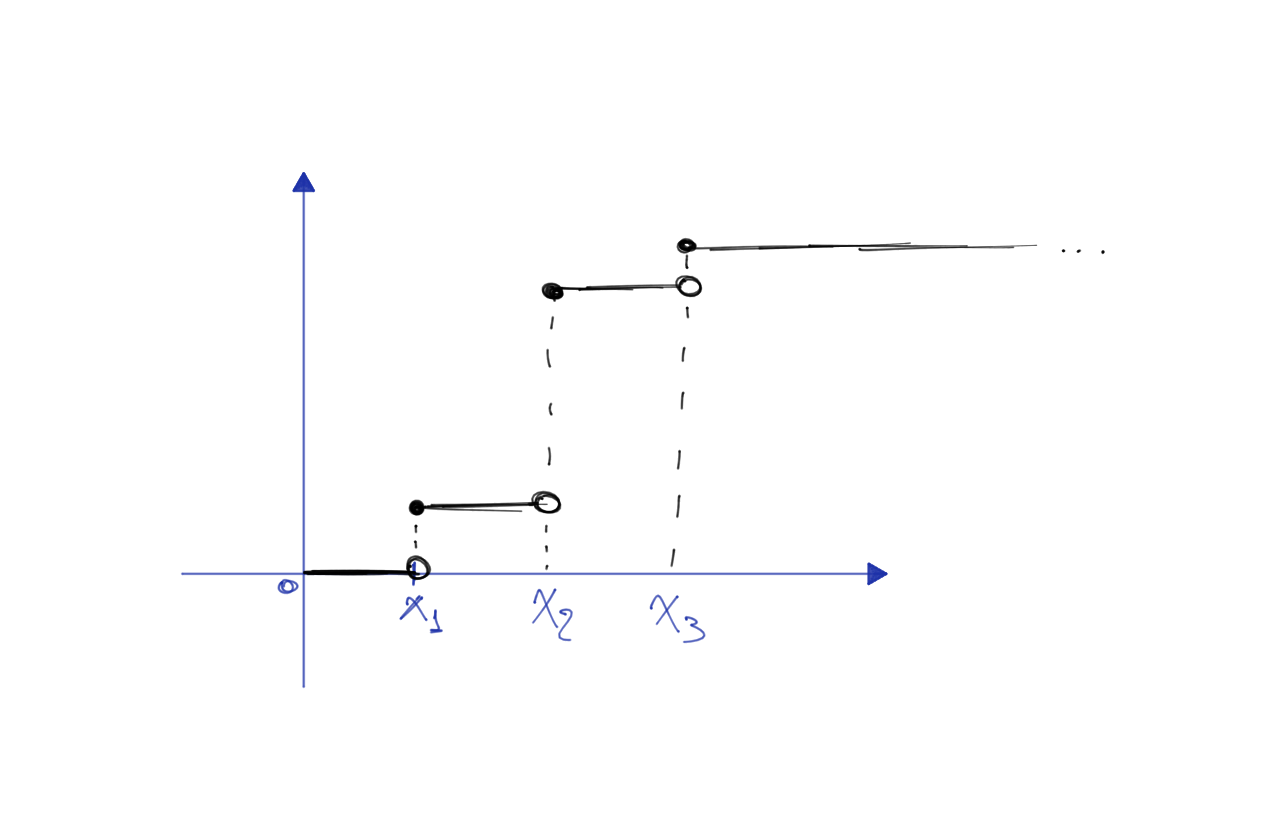
\includegraphics[width=0.5\textwidth]{figures/exponents.png}
        \caption{Filtration of Lyapunov exponents: the plot of $\dim E_\chi$ as a function of $\chi$ is a non-decreasing step function.}
        \label{fig:lyapunov_filtration}
    \end{figure}
If we restrict ourselves to linear gregs, i.e.\ gregs with cocycles $w: \mathbb T \times X \to \GL(d, \mathbb R)$ taking values in $\GL(d,\mathbb R)$,
then the pointwise version of Osedelec's multiplicative ergodic theorem tells us that the directed Lyapunov exponents exist for almost every point.
Its statement (and some more results) can be found as \cite[Theorem S.2.9]{katok1995introduction}:
\begin{theorem}[Osedelec's pointwise multiplicative theorem]\label{thm:osedelec}
    Let $(X, \mathcal X, m, T, w, \GL(d,\mathbb R))$ be a $\mathbb Z$-time greg, and assume that $(X, \mathcal X, m)$ is a Lebesgue space.
    If 
    \[
    \log^+ \|w(x)^{\pm 1}\| \in L^1(X, m),
    \]
    then there exists a co-null set $Y \subseteq X$ such that for every $x \in Y$:
    \begin{enumerate}[label=(\roman*)]
        \item There exists a decomposition 
        \[
        \mathbb R^d = \bigoplus_{i=1}^{k(x)} H_i(x),
        \]
        that is invariant under the action of $\mathbb Z$ on $X \times \mathbb R^d$.
        \item The Lyapunov exponents over $x$ exist, are finite, invariant under $T$, the same in all directions of $H_i(x) \setminus \{0\}$.
        In particular, 
        \[
        \lim_{n \to \pm \infty} \frac{1}{n} \log \|w(T^n(x))\| = \pm \chi_i(x)
        \]
        uniformly in $v \in H_i(x) \setminus \{0\}$.
    \end{enumerate}
\end{theorem}
\subsection{Osedelec's theorem and equivalent definitions of Lyapunov exponents}
Using Kingman's subadditive ergodic theorem, one can give for ergodic gregs a definition of Lyapunov exponents that does not depend on direction $v$ and the point $x$.
The statement of the following can be found as \cite[Theorem 4.3]{duarte2016lyapunov}, or \cite[Theorem 5.17]{bader2025lyapunov}
\begin{theorem}[Kingman's subadditive ergodic theorem]\label{thm:kingman}
Let $(X, \mathcal X, m, T, w, \GL(d,\mathbb R))$ be a $\mathbb Z$-time greg, with $(X, \mathcal X, m, T)$ ergodic.
If $f_n: X \to [-\infty, +\infty)$ is a sequence of measurable functions such that
\[
f_{n+m} \leq f_n + f_m \circ T^n,
\]
and $f_1^+ \in L^1(X, m)$, then for $m$-almost every $x \in X$ we have
\[
\lim_{n \to \infty} \frac{1}{n} f_n(x) = \inf_{n \in \mathbb N} \frac{1}{n} \int_X f_n dm
\]
where the limit exists and is finite.
\end{theorem}

\begin{definition}[(Nondirected) Lyapunov exponents for ergodic gregs]
    \ \\
    Let $(X, \mathcal X, m, T, w, \GL(d,\mathbb R))$ be a $\mathbb N$-time greg, with $(X, \mathcal X, m, T)$ ergodic.
    If 
    \[
    \log^+ \|w(x)\| \in L^1(X, m),
    \]
    then the limits
    \begin{align*}
        \chi_1 &= \lim_{n \to \infty} \frac{1}{n} \int_X \log \|w(n,x)\| dm(x),\\
        \chi_1 + \cdots + \chi_i &= \lim_{n \to \infty} \frac{1}{n} \int_X \log \|\wedge^i w(n,x)\| dm(x), \quad i = 2, \ldots, d,
    \end{align*}
    exist, are finite, and are called the \emph{Lyapunov exponents} of $w$.
    Moreover,
    \begin{enumerate}[label=(\roman*)]
        \item The limits above can be replaced with $\inf_{n \in \mathbb N}$.
        \item The Lyapunov exponents $\chi_i$ can be computed as
        \begin{align*}
            \chi_1 &= \lim_{n \to \infty} \frac{1}{n} \log \|w(n,x)\|,\\
            \chi_1 + \cdots + \chi_i &= \lim_{n \to \infty} \frac{1}{n} \log \|\wedge^i w(n,x)\|, \quad i = 1, \ldots, d.
        \end{align*}
        \item The Lyapunov exponents $\chi_i$ can also be computed as
        \begin{align*}
            \chi_1 &= \lim_{n \to \infty} \frac{1}{n} \log \sigma_1(w(n,x)),\\
            \chi_i &= \lim_{n \to \infty} \frac{1}{n} \log \sigma_i(w(n,x)), \quad i = 1, \ldots, d,
        \end{align*}
        where $\sigma_1(g) \geq \sigma_2(g) \geq \cdots \geq \sigma_d(g)$ are the singular values of $g \in \GL(d,\mathbb R)$.
    \end{enumerate}
\end{definition}
\begin{proof}[Proof of equivalence]
\begin{enumerate}[label=(\roman*)]
    \item Follows from \cref{thm:kingman} applied to the functions $f_n(x) = \log \|\wedge^i w(n,x)\|$.
    To see that the cocycles $\wedge^i w(n,x)$ will give a function in $L^1(X,m)$, note that $\|\wedge^i w(x)\| \leq \|w(x)\|^i$ for every $x \in X$.
    \item The equalities follow again from \cref{thm:kingman} applied to the functions 
    \[
    f_n(x) = \log \|w(n,x)\| \text{ and }f_n(x) = \log \|\wedge^i w(n,x)\|.
    \]
    \item The first equality follows from the previous point and the fact that $\sigma_1(g) = \|g\|$ for every $g \in \GL(d,\mathbb R)$, where the norm is the operator norm induced by the Euclidean norm on $\mathbb R^d$.
    For the rest, note that 
    \[
    \sigma_i(g) = \frac{\|\wedge^i g\|}{\|\wedge^{i-1} g\|} \text{ for } i = 2, \ldots, d,
    \]
    so $\log \sigma_i(g) = \log \|\wedge^i g\| - \log \|\wedge^{i-1} g\|$ for every $g \in \GL(d,\mathbb R)$, giving us that the result inductively.
\end{enumerate}
\end{proof}
\subsection{Equivalent cocycles}
    \begin{definition}[Tempered maps]
        Let $(X, \mathcal X, m, T, w, \GL(d,\mathbb R))$ be a greg.
        A measurable map $C: X \to \GL(d, \mathbb R)$ is called \emph{tempered} with respect to $T$ if for $m$-almost every $x \in X$ we have
        \[
        \lim_{ n \to \infty} \frac{1}{n} \log \|C(T^n(x))^{\pm 1}\| = 0.
        \]
    \end{definition}
    The following is \cite[Lemma S.2.4]{katok1995introduction}:
    \begin{lemma}[Criterion for temperedness]
        Let $(X, \mathcal X, m, T, w, \GL(d,\mathbb R))$ be a greg on $\mathbb R$.
        If $C: X \to \GL(d, \mathbb R)$ is such that
        \[
        \max \{\log \|C(x)\|, \log \|C(x)^{-1}\|\} \in L^1(X, m),
        \]
        then $C$ is tempered with respect to $T$.
    \end{lemma}
    \begin{proof}
        Use Birkhoff's ergodic theorem on the functions $\log \|C(x)\|$ and $\log \|C(x)^{-1}\|$.
    \end{proof}
    \begin{definition}[Equivalent cocycles]
        Consider two gregs $(A, \GL(d,\mathbb R))$ and $(B, \GL(d,\mathbb R))$ over the same flow and probability space $(X, \mathcal X, m, T)$.
        We say that the cocycles $A$ and $B$ are \emph{equivalent} if there exists a tempered map $C: X \to \GL(d, \mathbb R)$ such that for $m$-almost every $x \in X$ we have
        \[
        A(x) = C(T(x))^{-1} B(x) C(x)^{-1}.
        \]
        A cocycle is called \emph{rigid} if it is equivalent to a cocycle with generator independent from $x$, i.e.\ $B(n,x) = B^n$ for some $B \in \GL(d,\mathbb R)$ and every $n \in \mathbb N, x \in X$.
    \end{definition}

\section{2025-10-03}
\subsection[Proof of 2d(1,n) <= d(1,2)]{Proof of $2\delta_{1,n} \leq \delta_{1,2}$}
Note that critical exponents of functionals are defined for positive functionals on the Weyl chamber because we want that for $s > \delta_\Gamma(\varphi)$ the series converges.
\begin{lemma}[Properties of critical exponents]
    Let $\Gamma$ be a discrete subgroup of $\SL(d,\mathbb R)$.
    Then for functionals $\varphi, \psi: \mathfrak a \to \mathbb R$ that are positive on the Weyl chamber $\mathfrak a^+$ we have
    \begin{enumerate}[label=(\roman*)]
        \item $\delta_\Gamma(\lambda \varphi) = \frac{1}{\lambda} \delta_\Gamma(\varphi)$ for every $\lambda > 0$.
        \item If $\varphi \leq \psi$ on $\mathfrak a^+$, then $\delta_\Gamma(\varphi) \geq \delta_\Gamma(\psi)$.
    \end{enumerate}
\end{lemma}

We want to show that
\begin{proposition}\label{prop:critical_exponent_inequality}
    Let $\Gamma$ be a discrete subgroup of $\SL(d,\mathbb R)$.
    Then
    \[
    2 \delta_{1,n}(\Gamma) \leq \delta_{1,2}(\Gamma),
    \]
    where $\delta_{1,n}(\Gamma) = \delta_\Gamma(\alpha_{1,n})$ and $\delta_{1,2}(\Gamma) = \delta_\Gamma(\alpha_{1,2})$, and $\alpha_{i,j}(\mathrm{diag}(a_1, \ldots, a_d)) = a_i - a_j$.
\end{proposition}
By the above lemma, it would be enough to show that $\alpha_{1,n} \geq \frac{1}{2} \alpha_{1,2}$ on the Weyl chamber $\mathfrak a^+$, but this is not true.
A counter example in $\SL(3,\mathbb R)$ is given by the matrix $\mathrm{diag}(3, -2, -1)$, for which $\alpha_{1,3} = 4$ and $\alpha_{1,2} = 5$.

We will use the fact that for the opposition involution $\iota: \mathfrak a \to \mathfrak a$ in $\mathfrak{sl}(d,\mathbb R)$ we have
\[
\alpha_{i,j}(H) = \alpha_{d-j+1, d-i+1}(\iota(H)).
\]
We recall its general definition:
\begin{definition}[Opposition involution]
    Consider a choice of a Cartan subalgebra $\mathfrak a$ and a Weyl chamber $\mathfrak a^+$ of a semisimple Lie algebra $\mathfrak g$.
    There exists a unique element of the Weyl group $w_0$ that sends $\mathfrak a^+$ to $-\mathfrak a^+$.
    The \emph{opposition involution} is the map $\iota: \mathfrak a \to \mathfrak a$ defined by $\iota(H) = - w_0(H)$.
\end{definition}

We also recall that the Cartan decomposition is unique up to the action of the Weyl group. This is \cite[Proposition 7.39]{knapp1996lie}.
\begin{proposition}[Uniqueness of Cartan decomposition]
    Let $G$ be a reductive group.
    Then 
    \[
    K a K = K a' K \iff a' = w \cdot a \text{ for some } w \in W,
    \]
    where $W$ is the Weyl group of $G$ and $a, a' \in A$.
\end{proposition}

\begin{proof}[Proof of \cref{prop:critical_exponent_inequality}]
    Note that the proposition above tells us that for every $g \in \SL(d,\mathbb R)$:
    \[
    \alpha_{n-1,n}(\mu(g)) = \alpha_{1,2}(\mu(g^{-1})),
    \]
    since for $k,l \in K$ we have $g = k \exp(\mu(g)) l$ and 
    $$g^{-1} = l^{-1} \exp(-\mu(g)) k^{-1} = l^{-1} -w_0(\mu(g)) k^{-1} = l^{-1} \exp(\iota(\mu(g))) k^{-1}$$, so $\mu(g^{-1}) = \iota(\mu(g))$ which negates and inverses the entries of $\mu(g)$.

    Since $\alpha_{1,n} = \alpha_{1,2} + \alpha_{2,3} + \cdots + \alpha_{n-1,n} \geq \alpha_{1,2}+ \alpha_{n-1,n}$, Hölder's inequality gives us that for $1/p + 1/q = 1$ and $s > 0$:
    \begin{align*}
        \sum_{\gamma \in \Gamma} e^{-s \alpha_{1,n}(\mu(\gamma))} &\leq 
        \sum_{\gamma \in \Gamma} e^{-s (\alpha_{1,2}(\mu(\gamma)) + \alpha_{n-1,n}(\mu(\gamma)))}\leq\\
        &leq \left(\sum_{\gamma \in \Gamma} e^{-s \alpha_{1,2}(\mu(\gamma))}\right)^{1/p} \left(\sum_{\gamma \in \Gamma} e^{-s \alpha_{n-1,n}(\mu(\gamma))}\right)^{1/q}
    \end{align*}
    Note that the sum of the right-hand side converges if
    \[
    s > \max\{\frac{1}{p} \delta_{1,2}, \left(1 - \frac{1}{p}\right) \delta_{n-1,n}\}
    \]
    which is optimal (i.e.\ as small as possible) when $p^{-1} = \delta_{n-1,n }/(\delta_{1,2} + \delta_{n-1,n})$.
    Thus the sum on the left-hand side converges if
    \[
    s > \frac{\delta_{1,2} \delta_{n-1,n}}{\delta_{1,2} + \delta_{n-1,n}}.
    \]
    meaning that 
    \[
    \delta_{1,n} \leq \frac{\delta_{1,2} \delta_{n-1,n}}{\delta_{1,2} + \delta_{n-1,n}}.
    \]
    However, the fact that $\alpha_{1,2}(\mu(g)) = \alpha_{n-1,n}(\mu(g^{-1}))$ implies that $\delta_{1,2} = \delta_{n-1,n}$, so the result follows.
\end{proof}
\subsection{Geodesic flow on groups}
We would like to explain the definition of the geodesic flow on a hyperbolic group $\Gamma$.
To motivate it, we start with the case of the geodesic flow on a simply connected negatively curved manifold $M$, then pass to the case of a group $\Gamma$ acting properly discontinuously on a negatively curved manifold, and finally to the case of a hyperbolic group $\Gamma$.
\subsubsection{Geodesic flow on a simply connected negatively curved manifold}\todo{Why do we not allow zero curvature?}
Let $\tilde M$ be a simply connected, complete, negatively curved manifold.
Then by the Cartan-Hadamard theorem, $\tilde M$ is diffeomorphic to a ball $\mathbb B^n$ and the exponential map $\exp_x: T_x \tilde M \to \tilde M$ is a diffeomorphism for every $x \in \tilde M$.
Using $\exp_x$ we can identify the Gromov boundary $\partial_\infty \tilde M$ with the unit tangent sphere $\mathbb S^{n-1} \simeq T_x^1 \tilde M$ at $x$.
So we can think of $\tilde M \cup \partial_\infty \tilde M$ as the closed ball $\overline{\mathbb B^n}$, just like in the case of Poincaré-disc model of the hyperbolic space $\mathbb H^n$.

We have the following fiber bundle over the space $\partial_\infty \tilde M^{(2)}$ of distinct pairs of boundary points, with fiber isomorphic to $\mathbb R$:

\begin{center}
\begin{tikzcd}[column sep=large, row sep=large]
    T^1 \tilde M \arrow[d, "\pi"] & \mathbb R \arrow[l, two heads] \\
    \partial_\infty \tilde M^{(2)}
\end{tikzcd}    
\end{center}
where 
\[
\pi: T^1 \tilde M \to \partial_\infty \tilde M^{(2)}, \quad v \mapsto \left(\lim_{t \to +\infty} \phi_t(v), \lim_{t \to -\infty} \phi_t(v)\right),
\]
and $\phi_t: T^1 \tilde M \to T^1 \tilde M$ is the geodesic flow on $\tilde M$. The fiber over a pair of distinct boundary points $(\xi^-, \xi^+) \in \partial_\infty \tilde M^{(2)}$ are the unit tangent vectors pointing towards $\xi^+$ that are tangent to the geodesic connecting $\eta$ and $\xi^+$.

This is a principal bundle. 
The reals $\mathbb R$ should be thought rather as the affine line, since the choice of a base point $0$ is not canonical.

To trivialize the bundle, we consider a section $s: \partial_\infty \tilde M^{(2)} \to T^1 \tilde M$ which gives us a base point $s(\xi^-, \xi^+)$ in each fiber $\pi^{-1}(\xi^-, \xi^+)$.
Then we can identify $T^1 \tilde M$ with $\partial_\infty \tilde M^{(2)} \times \mathbb R$ via the map
\begin{align*}
    \partial_\infty \tilde M^{(2)} \times \mathbb R &\to T^1 \tilde M,\\
    (\xi^-, \xi^+, t) &\mapsto \phi_t(s(\xi^-, \xi^+)).
\end{align*}
Thus, given a section $s: \partial_\infty \tilde M^{(2)} \to T^1 \tilde M$, we associate to each $v \in T^1 \tilde M$ the triple $(\xi^-, \xi^+, t)$, where $\xi^\pm$ are the endpoints of the (oriented) geodesic tangent to $v$ and $t$ is the signed distance between $s(\xi^-, \xi^+)$ and $v$ along the geodesic.

\subsubsection{Geodesic flow on a negatively curved manifold\\Or a group acting properly discontinuously on a negatively curved simply connected manifold}
Consider now a complete, negatively curved manifold $M$.
Then $M$ is isometric to the quotient $\Gamma \backslash \tilde M$, where $\tilde M$ is the universal cover of $M$ and $\Gamma = \pi_1(M)$ acts on $\tilde M$ by isometries.

Note that this is equivalent to considering a torsion-free group $\Gamma$ acting by isometries, properly discontinuously on a simply connected, complete, negatively curved manifold $\tilde M$.
This is the setting that we will work on.
From an analog of the Milnor-Svarc lemma for non-cocompact actions, we know that the orbit maps $\Gamma \to \tilde M$ are quasi-isometric embeddings.
Extending these to topological embeddings of the boundaries gives us an embedding of the boundaries $\partial_\infty \Gamma \subseteq \partial_\infty \tilde M$, which does not depend on the choice of the orbit.

Our goal is to define a properly discontinuous action of $\Gamma$ on $T^1 \tilde M$ that commutes with the geodesic flow $\phi_t: T^1 \tilde M \to T^1 \tilde M$.
Then we will have defined a geodesic flow on $M = \Gamma \backslash \tilde M$ as the quotient flow $\Gamma \backslash T^1 \tilde M$.
We will use the (arbitrary) choice of a section $s: \partial_\infty \tilde M^{(2)} \to T^1 \tilde M$ to obtain a trivialization $\Phi: \tilde M^{(2)} \times \mathbb R \to T^1 \tilde M$.
We define the action of $\gamma$ on $\partial_\infty \tilde M^{(2)} \times \mathbb R$ as
\begin{align*}
    \Phi^{-1} \gamma \Phi: \partial_\infty \tilde M^{(2)} \times \mathbb R &\to \partial_\infty \tilde M^{(2)} \times \mathbb R,\\
    (\xi^-, \xi^+, t) &\mapsto (\gamma \xi^-, \gamma \xi^+, t + c(\gamma, \xi^-, \xi^+)),
\end{align*}
where $c: \Gamma \times \partial_\infty \tilde M^{(2)} \to \mathbb R$.
Since this clearly lifts the action of $\Gamma$ on $\tilde M$, we know from the theory of cocycles that $\Phi^{-1} \gamma \Phi$ is an action if and only if $c$ is a cocycle.
To see this, one can use the definition of $\Phi$, or the fact that $\gamma$ acts by isometries.
\begin{remark}[Action and arbitrariness of parametrisation]
    Note that while the action of $\Gamma$ on $T^1 \tilde M$ is canonical, the action on $\partial_\infty \tilde M^{(2)} \times \mathbb R$ depends on the choice of the section $s: \partial_\infty \tilde M^{(2)} \to T^1 \tilde M$.
    To see this consider another section $s': \partial_\infty \tilde M^{(2)} \to T^1 \tilde M$, which we denote with $s'(x) = (x, \bar s'(x))$, and let
    \[
    f: \partial_\infty \tilde M^{(2)} \to \mathbb R, \quad f(x) = \bar s'(x) - \bar s(x).
    \]
    Then using the definition of $\Phi$ one can check that $\phi_t \Phi(x,t) = \Phi T_{f(x)}(x,t)$, where $T_s: \mathbb R \to \mathbb R$ is the translation $T_s(t) = t + s$, and that $\Phi'(x,t) = \phi_{f(x)} \Phi(x,t)$.
    Using this one can calculate that
    \[
    \Phi'^{-1} \gamma \Phi'(x,t) = ( \gamma x, t + c(\gamma, x) + f(x) - f(\gamma x)).
    \]
    Hence $c'(\gamma, x) = c(\gamma, x) + f(x) - f(\gamma x)$, i.e.\ $c$ and $c'$ are cohomologous cocycles.

    In this sense, the parametrised action of $\Gamma$ on $\partial_\infty \tilde M^{(2)} \times \mathbb R$ is well-defined up to cocycle cohomology class.
\end{remark}

The following lemma shows that the action of $\Gamma$ on $T^1 \tilde M$ is properly discontinuous.
\begin{lemma}
    If a group $\Gamma$ acts properly discontinuously on a manifold $N$, then it acts properly discontinuously on $T^1 N$.
\end{lemma}
Moreover, since $\Gamma$ acts by isometries, the action on $T^1 \tilde M$ commutes with the geodesic flow $\phi_t: T^1 \tilde M \to T^1 \tilde M$, which thus descends to a flow on $\Gamma \backslash T^1 \tilde M = T^1 M$.
Denoting with $\pi: T^1 \tilde M \to \partial_\infty \tilde M^{(2)}$ the projection, one can show that
\begin{fact}
The set 
\[
\Gamma \backslash \partial_\infty \Gamma^{(2)} \times \mathbb R \simeq \Gamma \backslash \pi^{-1}(\partial_\infty \Gamma^{(2)}) \subseteq T^1 M
\]
is compact and coincides with the non-wandering set of the geodesic flow on $T^1 M$.
\end{fact}
In the case where $\Gamma$ is cocompact, this is the whole $T^1 M$, since $\partial_\infty \Gamma = \partial_\infty \tilde M$.
Then things are a bit easier:
\begin{exercise}
Let $\Gamma$ be a torsion-free discrete group acting cocompactly by isometries on a complete negatively curved manifold $\tilde M$.
Then $\Gamma$ acts properly discontinuously and cocompactly on $T^1 M$.
\end{exercise}
\begin{proof}[Solution]
    We will denote with $\pi: T^1 M \to M$ the bundle projection.
    It is easy to see that the quotient map $T^1 M \to T^1 M / \Gamma$ lifts the quotient map $M \to M / \Gamma$, making the following diagram commute:
    \begin{center}
    \begin{tikzcd}[column sep=large, row sep=large]
        T^1 M \arrow[d, "\pi"] \arrow[r] & T^1 M / \Gamma \arrow[d, "\bar \pi"] \\
        M \arrow[r] & M / \Gamma
    \end{tikzcd}    
    \end{center}
    To prove proper discontinuity, let $K \subseteq T^1 M$ be compact and $\gamma_n \in \Gamma$ be a sequence in $\Gamma$ such that $\gamma_n K \cap K \neq \emptyset$.
    Then $\pi(\gamma_n K) \cap \pi(K) \neq \emptyset$, so $\{\gamma_n \}$ is finite since $\Gamma$ acts properly discontinuously on $M$.

    For cocompactness, let $K \subseteq M$ be a compact set such that $\Gamma K = M$ and $v_n \in T^1 M$ be a sequence.
    Then we can find $\gamma_n \in \Gamma$ such that $\gamma_n \pi(v_n) = \pi (\gamma_n v_n) \in \pi(K)$, which up to a subsequence will converge to a point $p \in \pi(K)$.
    Using an orthonormal frame around $p$, we can trivialize a neighborhood of $p$ in $T^1 M$ as $\Phi: \pi^{-1}(U) \to U \times \mathbb S^{n-1}$.
    Then $\Phi(\gamma_n v_n)$ will converge to a point in $\{p\} \times \mathbb S^{n-1}$, so $[\gamma_n v_n]$ will converge to a point in $T^1(M)/\Gamma$.

    Alternatively, one can show that $T^1 M / \Gamma$ is homeomorphic to $T^1(M/\Gamma)$, which is compact since $M/\Gamma$ is compact.
\end{proof}

\subsection{Geodesic flow on a hyperbolic group}
Let $\Gamma$ be a hyperbolic group acting properly discontinuously and cocompactly on a hyperbolic space (this is the case for instance when $X$ is the Cayley graph of $\Gamma$ with respect to a finite generating set).
A consequence of the Milnor-Svarc lemma is that $\partial_\infty \Gamma \simeq \partial_\infty X$.
\begin{remark}[Analogies to negatively curved manifolds]
    Here $X$ is an analog of the universal cover of a negatively curved manifold, and $\Gamma$ is an analog of the fundamental group acting by isometries on $X$.    
\end{remark}



The analog of the unit tangent bundle is defined as the set of parametrized unit-speed geodesics
\[
T^1 X = \{v : \mathbb R \to X \mid v \text{ is an isometry}\},
\]
which comes with the analog of the bundle projection and the geodesic flow 
\begin{align*}
    \pi: T^1 X &\to X, \quad v \mapsto (v(-\infty), v(+\infty)),\\
    \phi_t: T^1 X &\to T^1 X, \quad v \mapsto (s \mapsto v(s+t)).
\end{align*}
One can show that the action of $\Gamma$ on $X$ induces a properly discontinuous  and cocompact action on $T^1 X$ that commutes with the geodesic flow.
As before, we can consider the fiber bundle
\begin{center}
\begin{tikzcd}[column sep=large, row sep=large]
    T^1 X \arrow[d, "\rho"] & \mathbb R \arrow[l] \\
    \partial_\infty X^{(2)} \simeq \partial_\infty \Gamma^{(2)}
\end{tikzcd}    
\end{center}
where the projection is defined as before
\[
\rho: T^1 X \to \partial_\infty X^{(2)}, \quad v \mapsto \left(\lim_{t \to +\infty} \phi_t(v), \lim_{t \to -\infty} \phi_t(v)\right),
\]
and for a section $s: \partial_\infty \Gamma^{(2)} \to T^1 X$ we have a trivialization $\Phi: \partial_\infty \Gamma^{(2)} \times \mathbb R \to T^1 X$.
Then one can show
\begin{fact}
    There exists a cocycle $c: \Gamma \times \partial_\infty X^{(2)} \to \mathbb R$ such that the action of $\Gamma$ on $T^1 X$ is properly discontinuous, cocompact and commutes with the geodesic flow.
\end{fact}

\section{2024-10-07}
Let $S$ be a closed surface of genus $g \geq 2$.
Then by the classical Teichmüller theory, the Teichmüller space $\mathcal T(S)$ of $S$ has at least two models:
\[
\left\{
\begin{array}{l}
    \text{Discrete faithful}\\
    \text{representations } \\
    \pi_1(S) \to \text{PSL}(2, \mathbb R) \\
\end{array}
\right\}
//\PSL(2, \mathbb R) \simeq \left\{ 
    \begin{array}{l}
    \text{Hyperbolic markings}\\
    \text{on } S    
    \end{array}
    \right\}/\text{Diff}_0(S).
\]
Thus for a given representation $\rho: \pi_1(S) \to \PSL(2, \mathbb R)$, we can consider the associated hyperbolic surface $\Sigma = \rho(\pi_1(S)) \backslash \mathbb H^2$ which carries a class of hyperbolic metrics.


\end{document}